\documentclass[12pt,a4paper]{report}
\usepackage[brazilian, english]{babel}
\usepackage[utf8]{inputenc}
\usepackage[T1]{fontenc}
\usepackage{amsmath,amsthm,amsfonts,amssymb,textcomp}
%\usepackage{latexsym}
\usepackage{graphicx}
\graphicspath{{figuras}}
\usepackage{subfigure}
\usepackage{float}
\usepackage{longtable}
\usepackage{color}
\usepackage{epstopdf}
\usepackage{pdflscape}
\usepackage[breaklinks=true]{hyperref}
\usepackage[comma,authoryear]{natbib}
\usepackage[nonumberlist]{glossaries}
\usepackage{arydshln}
\usepackage{footnote}
\usepackage{longtable}
\usepackage[small,bf,singlelinecheck=off]{caption}
\usepackage[left=3cm,right=2cm,top=3cm,bottom=2cm]{geometry}
%\usepackage[alf]{abntcite}

%%% newcommand %%%%%%%%%%%%%%%%%
\newcommand{\PE}{Perkin-Elmer }
\newcommand{\BC}{Boller \& Chivens }

\newcommand{\degr}{\ensuremath{^{\circ}}}%                    % degree symbol:  °
\newcommand{\arcmin}{\ensuremath{^{\prime}}}%                    % degree symbol:  °
\newcommand{\arcsec}{\ensuremath{^{\prime\prime}}}%                    % degree symbol:  °
\newcommand{\fs}{\mbox{\ensuremath{.\!\!^s}}}
\newcommand{\farcm}{\mbox{\ensuremath{.\mkern-4mu^\prime}}}%    % fractional arcminute symbol: 0.'0
\newcommand{\farcs}{\mbox{\ensuremath{.\!\!^{\prime\prime}}}}%  % fractional arcsecond symbol: 0.''0
\newcommand{\fdg}{\mbox{\ensuremath{.\!\!^\circ}}}%             % fractional degree symbol:     0.°0



%\makeglossaries

\makeatletter
\renewcommand\chapter{\thispagestyle{plain}
                \global\@topnum\z@
                \@afterindentfalse
                \secdef\@chapter\@schapter}
\makeatother


\makeatletter
\renewcommand{\@makechapterhead}[1]{%
\vspace*{50 pt}%
{\setlength{\parindent}{0pt} \raggedright \normalfont
\bfseries\Huge\thechapter.\ #1
\par\nobreak\vspace{40 pt}}}
\makeatother

%\newglossaryentry{Offset}{name={Offset}, description={Diferença entre a posição obtida pela redução da observação e a posição dada pela efeméride}}
\newglossaryentry{OPD}{name={OPD}, description={Observatório do Pico dos Dias - Brasópolis, MG}}
\newglossaryentry{LNA}{name={LNA}, description={Laboratório Nacional de Astrofísica - Itajubá, MG}}
\newglossaryentry{OHP}{name={OHP}, description={Observatoire Haute Provence - Saint-Michel-l'Observatoire, França}}
\newglossaryentry{RA}{name={RA}, description={Sigla para Ascensão Reta ($ \alpha $)}}
\newglossaryentry{DEC}{name={DEC}, description={Sigla para Declinação ($ \delta $)}}
\newglossaryentry{Anomalia Verdadeira}{name={Anomalia Verdadeira}, description={Ângulo formado entre o Periastro e a posição instantânea do objeto na órbita centrado no planeta e contada na direção do movimento orbital}}
\author{Altair Ramos Gomes Júnior}
\title{Astrometry of the Neptune-Triton System}
\begin{document}

\maketitle

\pagestyle{headings}

\section*{Introduction}

In this report I present the preliminary results of the astrometric reductions of the images from the Observatório do Pico dos Dias (OPD) in Brazil. The aim is to obtain precise positions for the Neptune - Triton system and to investigate the orbit of Neptune alone around the Sun. The telescopes used were the \PE (160) with a diameter of 1.6m, the \BC (IAG) with a diameter of 0.6m, and the Zeiss telescope with a diameter of 0.6m.

The observations were carried out since 1992 when a CCD big enough was installed in the OPD. The planet and satellite have been constantly observed, and still are, by our group. There were many CCDs (IKON, IXON, CCD101, CCD106, ...) and many filters (V, R, I, No Filter, ...) utilized.

There was more than 5000 images from June 1992 to September 2015. Many of the oldest images had no coordinates in header or they were wrong. Sometimes the filter was missing. Many nights had two exposure sets. The first one with low exposure times so Neptune was not saturated, but there were few reference stars in the field. The second one with higher exposure time so Triton was brighter and had more reference stars than with the the previous exposure, but the image of Neptune were saturated.

In Table \ref{Tab:dados} it is summarized the final number of images for Neptune (short-exposure observations) and Triton (all observations) for the 3 telescopes. It is also shown the number of positions where Neptune and Triton were identified automatically in the same image (short-exposure observations for precision premium; see Section Tests).

\begin{table*}[h]
\centering
\caption{Number of positions by object by telescope}
\label{Tab:dados}
\begin{tabular}{|c|c|c|c|}
\hline 
Telescope & Neptune & Triton & Matches \\ 
\hline
160 & 782 & 1341 & 768 \\ 
\hline 
IAG & 3162 & 3645 & 2909 \\ 
\hline 
Zeiss & 354 & 479 & 341 \\ 
\hline 
Total & 4298 & 5465 & 4018 \\ 
\hline 
\end{tabular}
\\Number of positions identified of Neptune and Triton by telescope. Matches: Number of positions where Neptune and Triton were identified automatically in the same image.
\end{table*}



Fig. \ref{Fig:pos-dist} shows the distribution of positions where Neptune and Triton are identified in the same image (short-exposure observations) over the years. Figs \ref{Fig:filtro-160}-\ref{Fig:filtro-IAG} summarizes the distribution of positions with Neptune and Triton in the same image by filter obtained in the \PE , and \BC telescopes, respectively. Zeiss only has images observed in Clear and I filters.

\begin{figure}
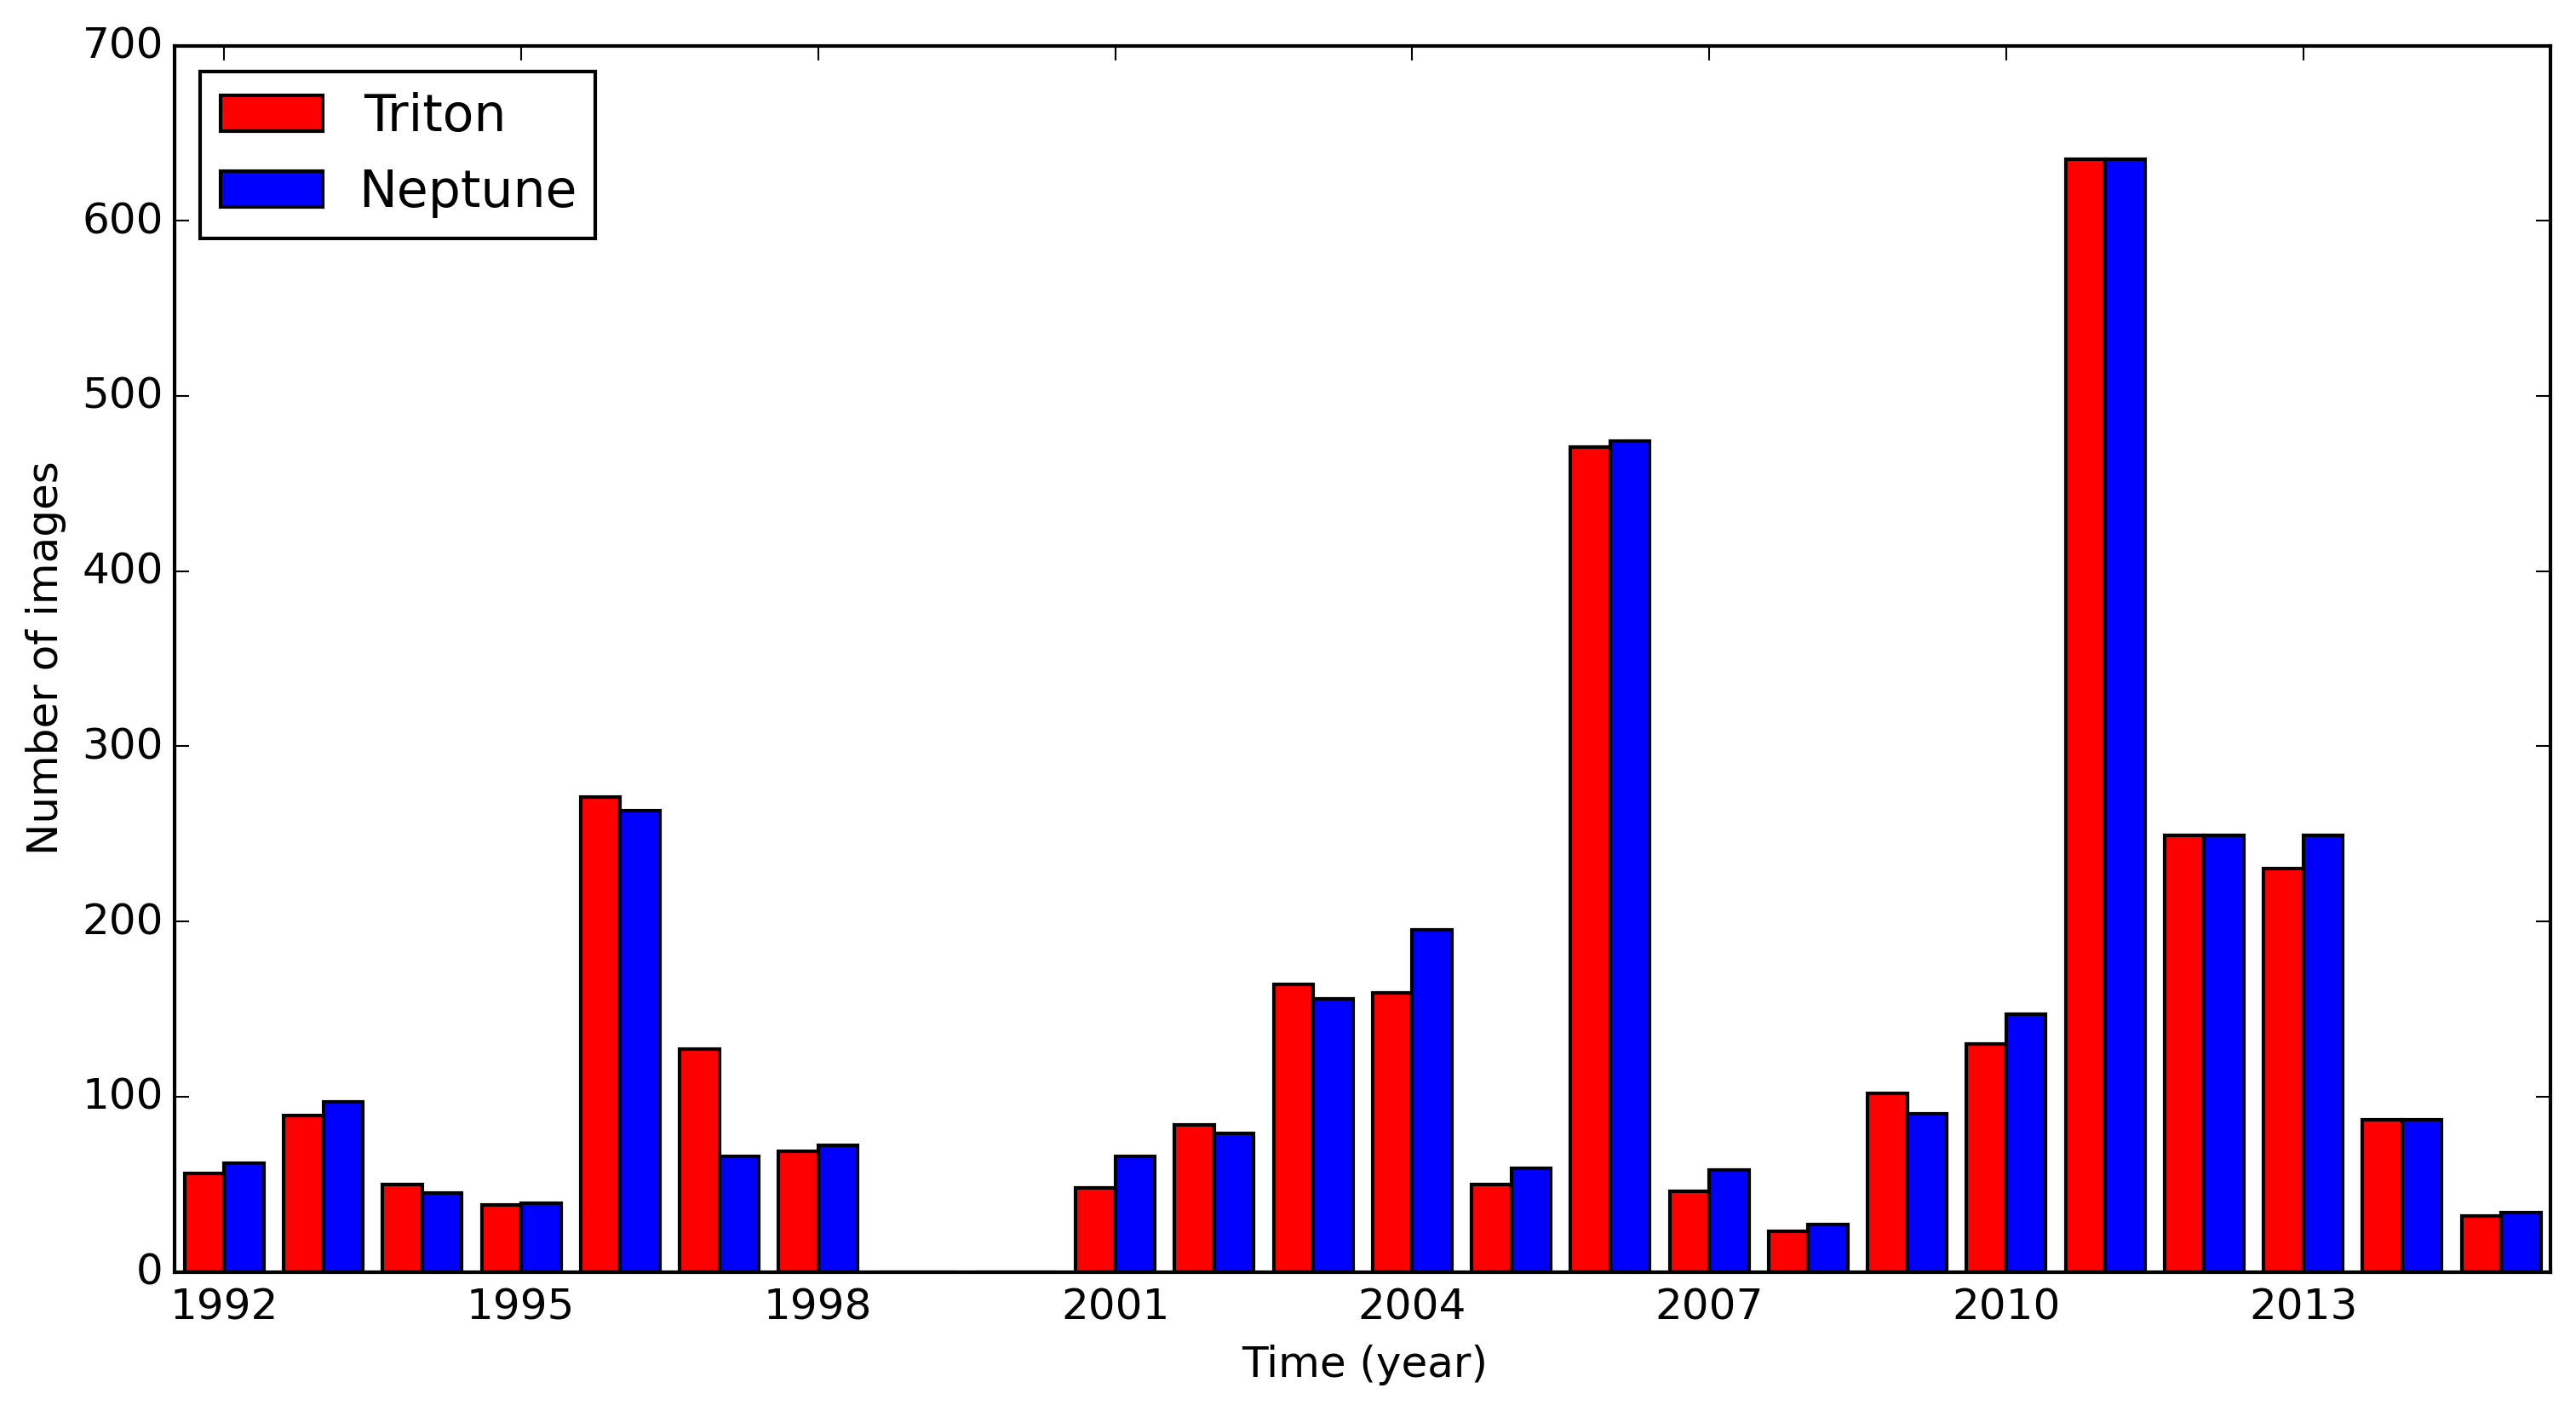
\includegraphics[width=16.0cm]{pos-distribution.png} 
\caption{Distribution of positions with Neptune and Triton in the same image (short-exposure observations) by year.}
\label{Fig:pos-dist}
\end{figure}



\begin{figure}[H]
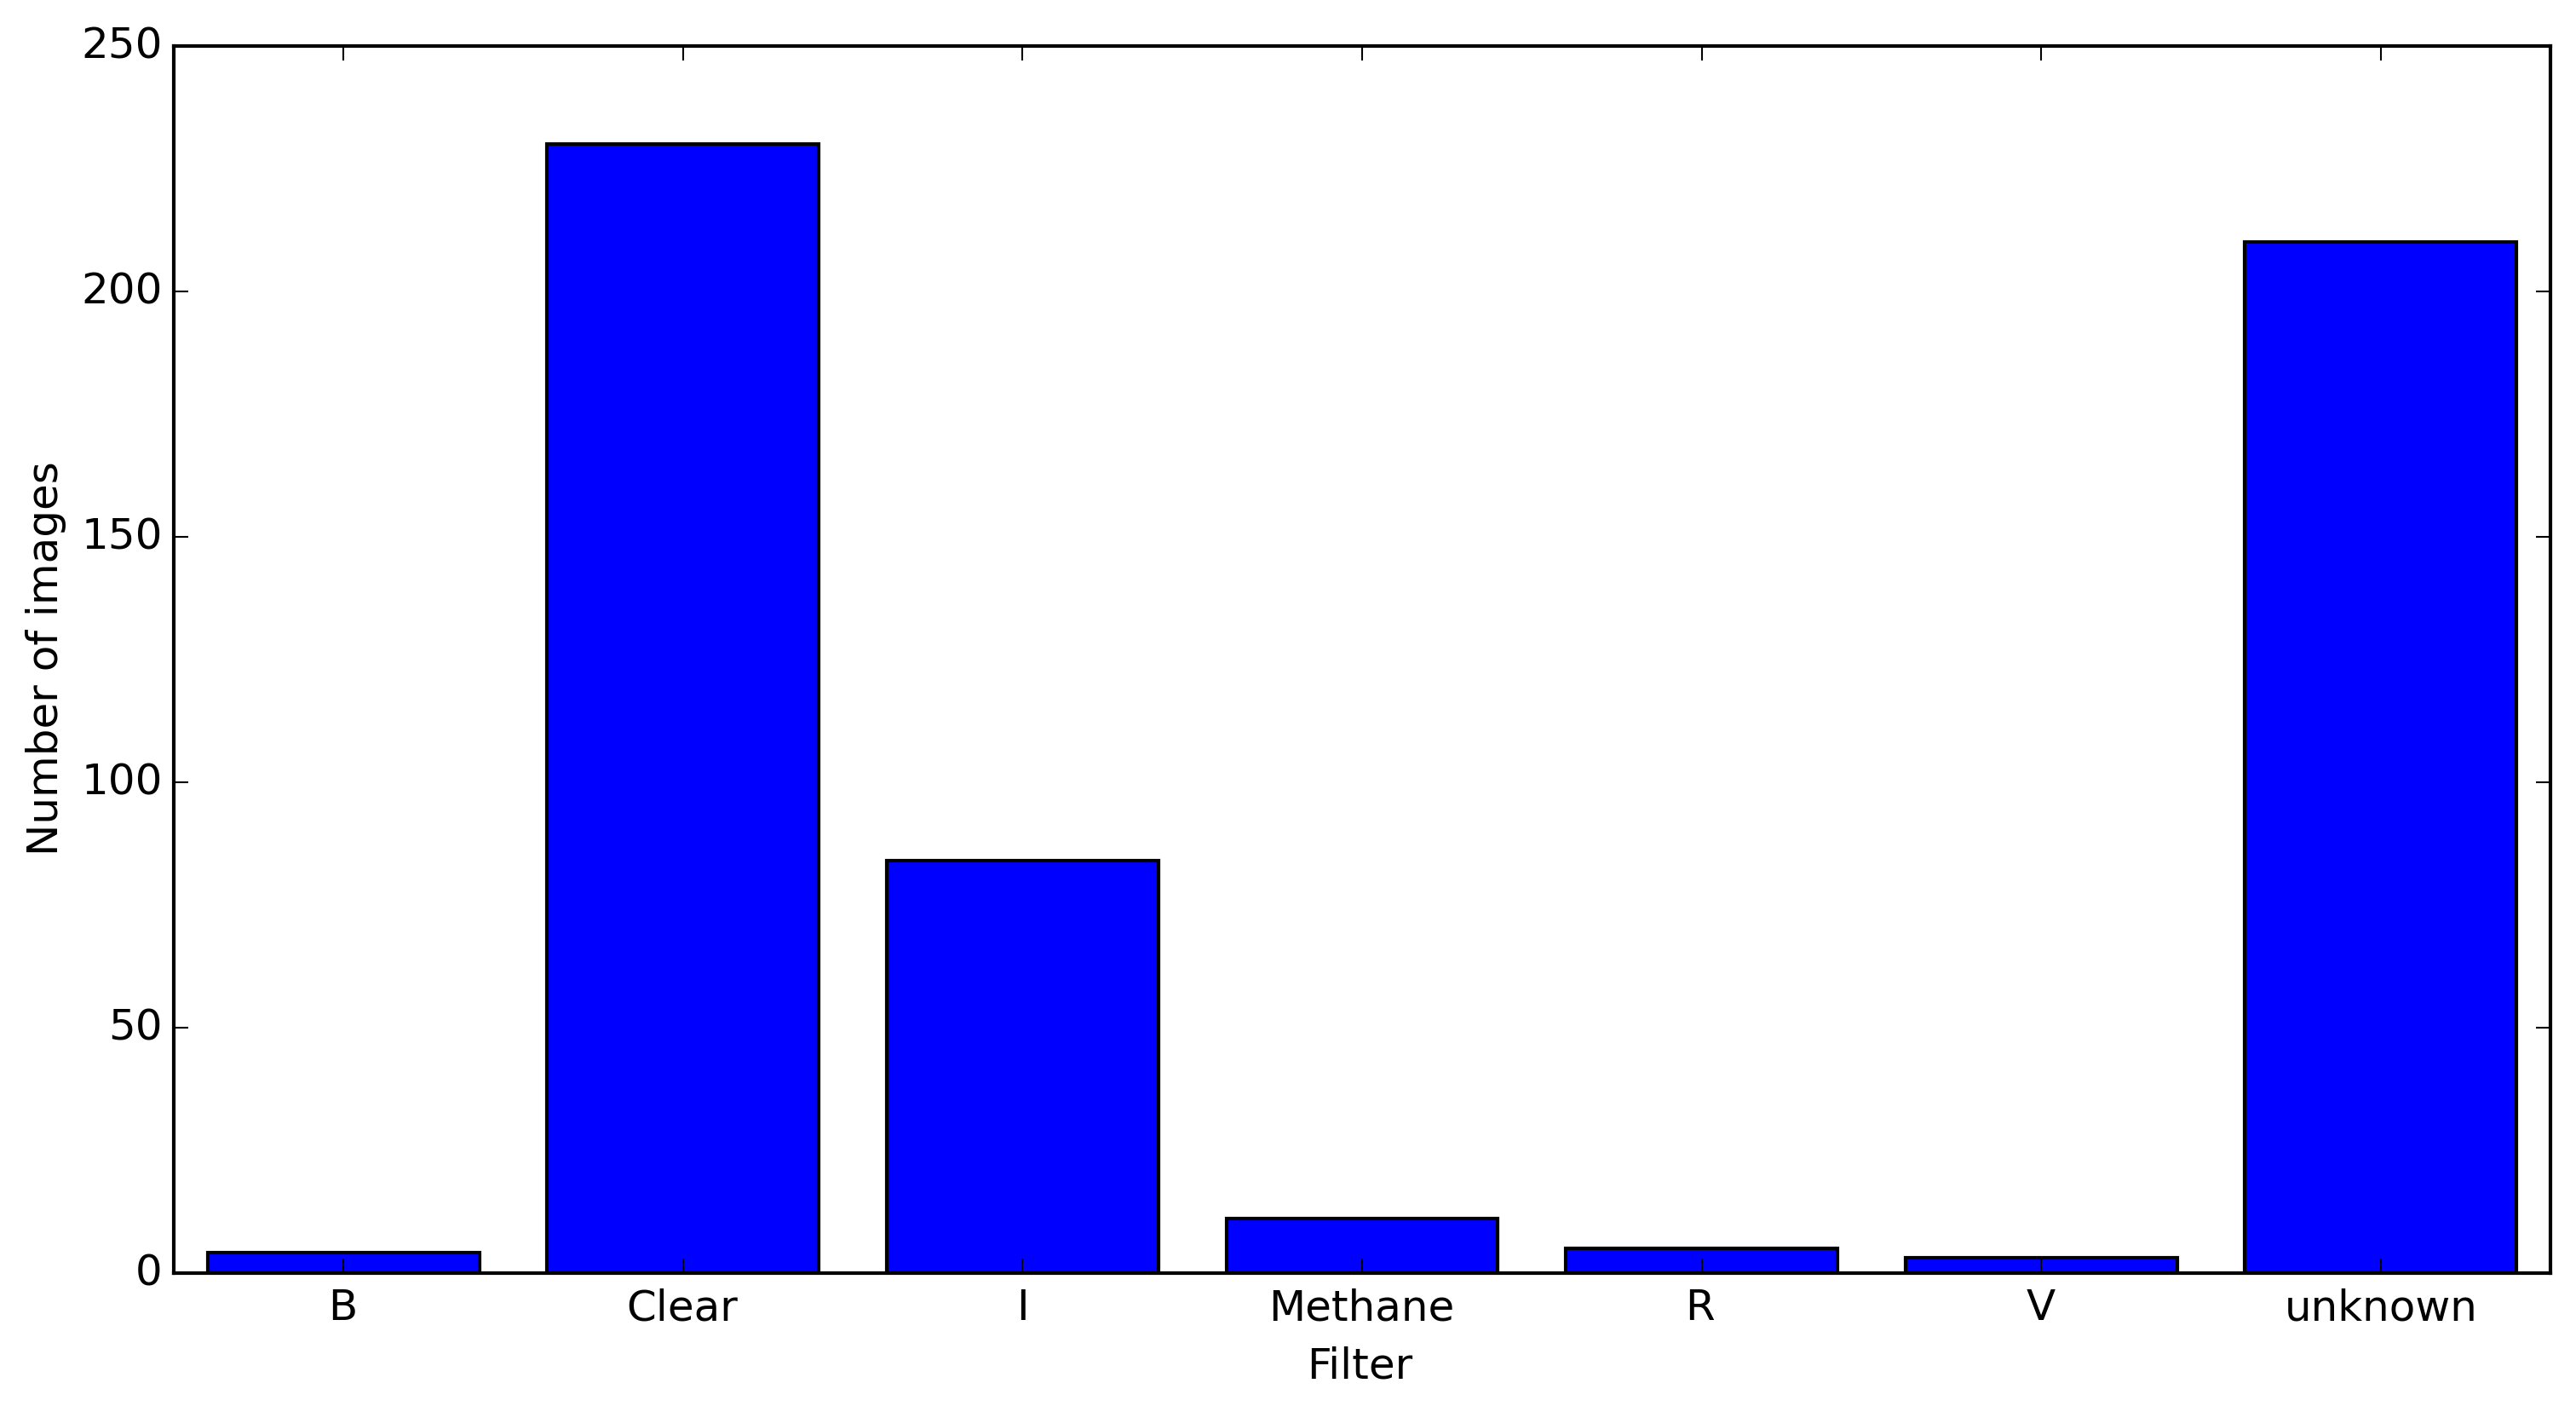
\includegraphics[width=16.0cm]{filtro_160.png} 
\caption{Distribution of positions with Neptune and Triton in the same image (short-exposure observations) by filter for the \PE telescope.}
\label{Fig:filtro-160}
\end{figure}

\begin{figure}[H]
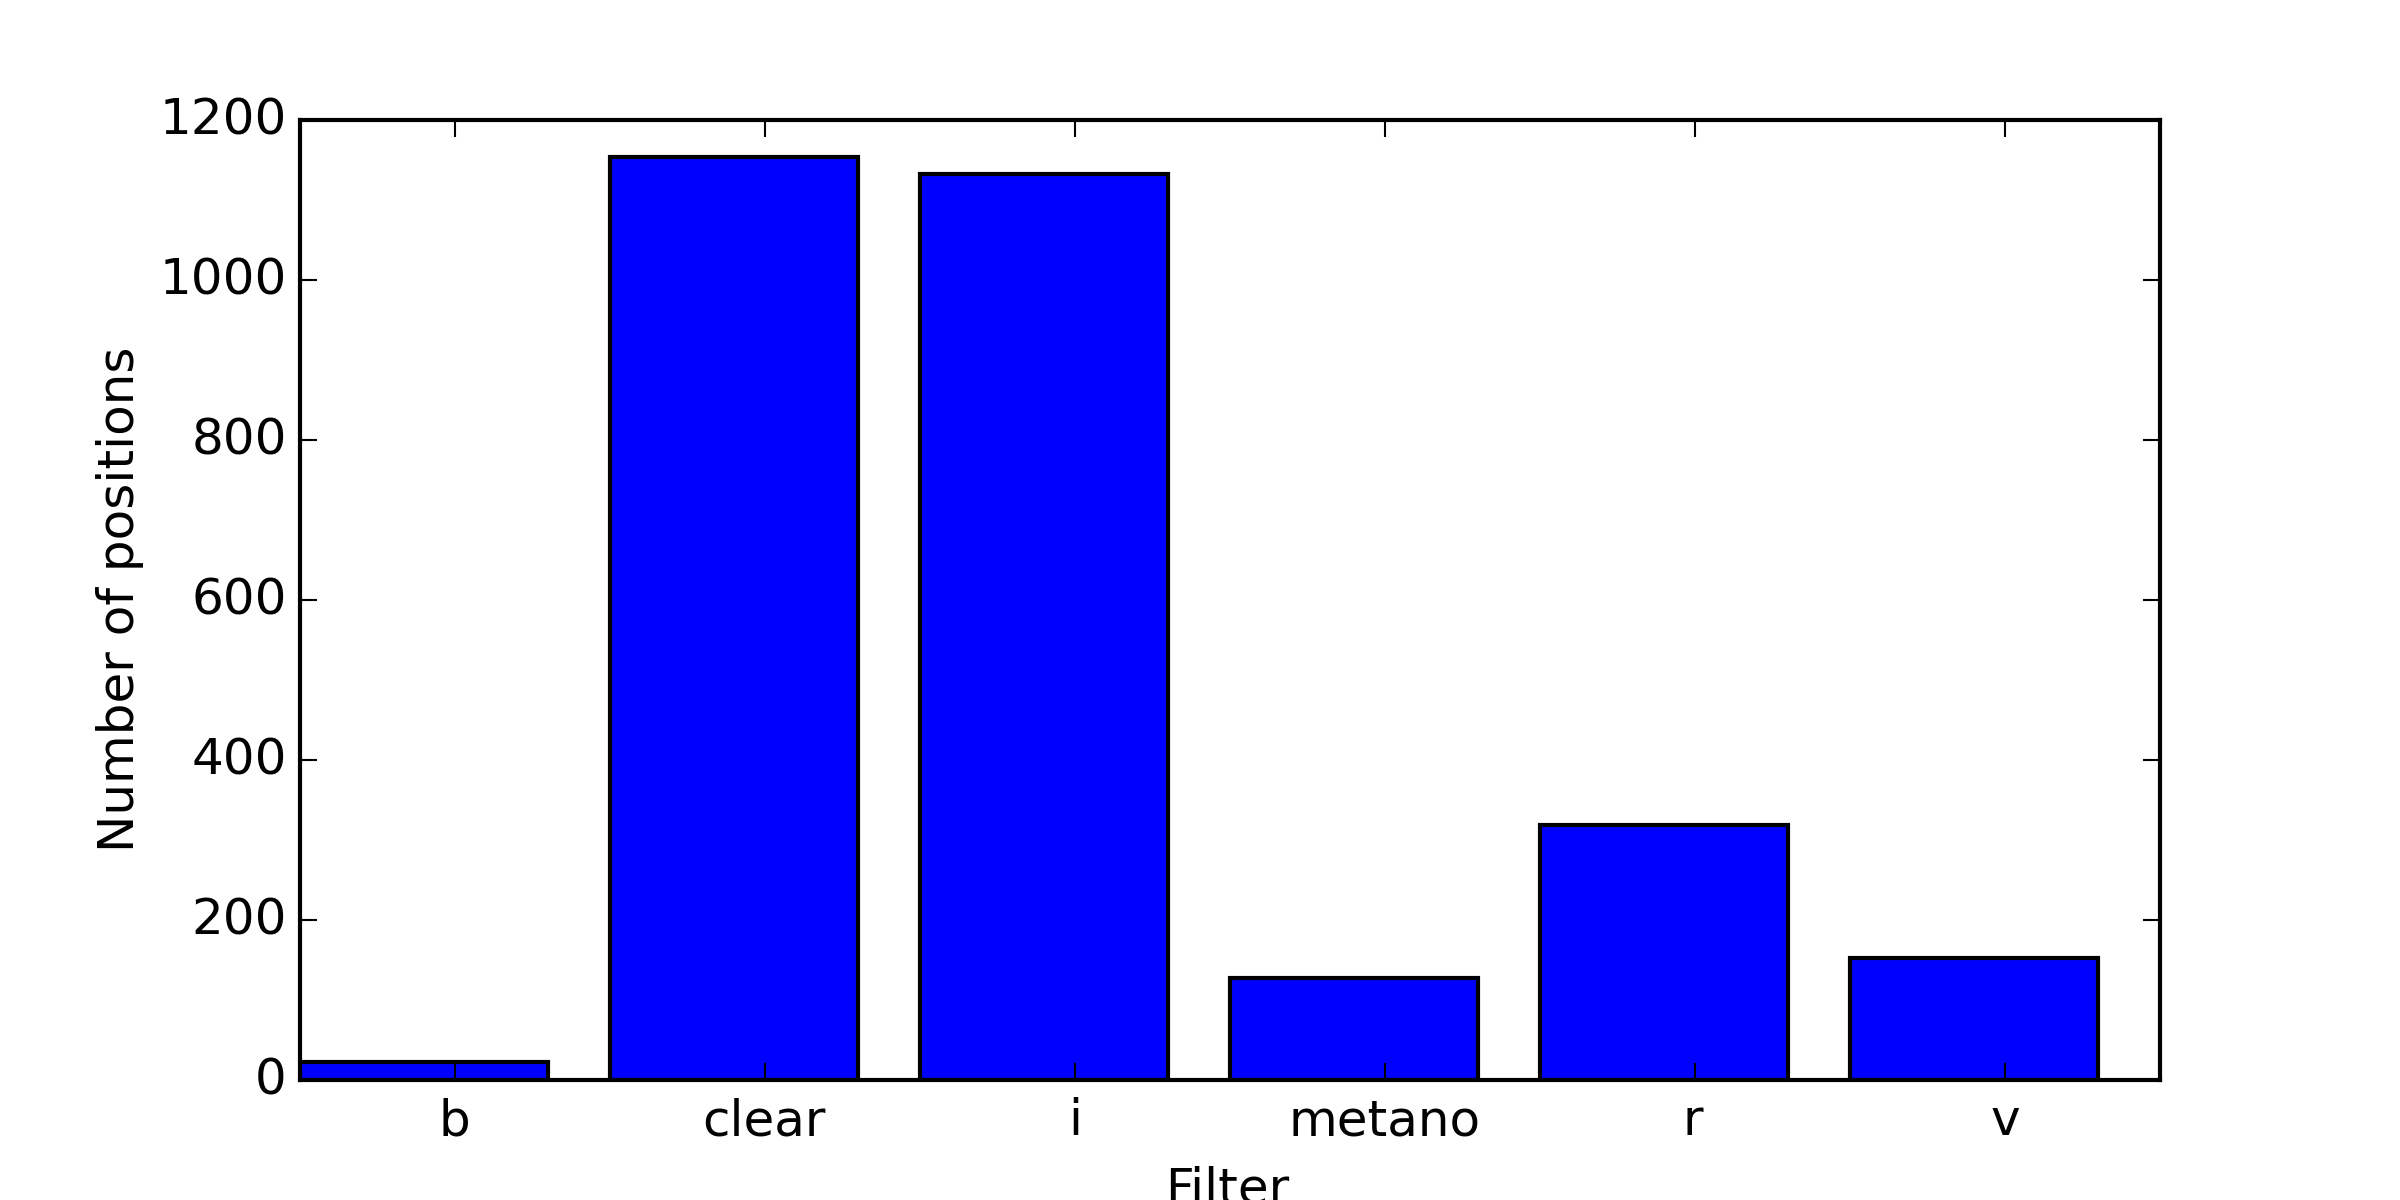
\includegraphics[width=16.0cm]{filtro_IAG.png} 
\caption{Same as in Fig \ref{Fig:filtro-160} for the \BC telescope.}
\label{Fig:filtro-IAG}
\end{figure}



\section*{Reduction}

The images were reduced using PRAIA, developed by Marcelo Assafin. To avoid the missing or wrong coordinates I used the coordinates of the ephemeris as input. This way PRAIA could identify reference stars in the images. The reference catalogue used was UCAC4. The ephemeris used to identify Neptune and Triton in the images was DE430+NEP081. The positions where the image of Neptune were saturated was removed of the results.

In Table 2 it is presented the mean errors in X and Y of the bidimensional Gaussian used to fit the PSF of the objects using only short-exposure observations.

\begin{longtable}{|l|c|c|c|c|}
\caption{Table of erros of the reduction. Gaussian error stands for the error in X and Y of the bidimensional Gaussian used to fit the PSF. Mean offset errors is the average dispersion of the positions of each night  using only short-exposure observations.}\\
\hline
Telescope/Satellite &  \multicolumn{2}{|c|}{Gaussian error} &   \multicolumn{2}{|c|}{Mean offet errors} \\
%\hline
 &  X (mas) & Y (mas) & RA (mas) & DEC (mas) \\
\hline
\endfirsthead
\multicolumn{5}{c}%
{\tablename\ \thetable\ -- \textit{Continued from previous page}} \\
\hline
Telescope/Satellite &  X & Y & RA & DEC \\
\hline
\endhead
\hline \multicolumn{5}{r}{\textit{Continued on next page}} \\
\endfoot
\hline
\endlastfoot
160/Neptune & 8 & 8 & 42 & 37 \\
160/Triton & 14 & 14 & 28 & 29 \\
IAG/Neptune & 9 & 9 & 36 & 38 \\
IAG/Triton & 20 & 20 & 34 & 37 \\
Zeiss/Neptune & 9 & 9 & 28 & 32 \\
Zeiss/Triton & 27 & 27 & 28 & 35 \\
\hline
\end{longtable}

We applied the digital coronagraphy technique to test if the scattered light of Neptune would influence in the Triton's photocenter. No influence was identified in the 1 mas range.

%From the offsets in the sense "position minus ephemeris" identified I made statistics night by night to eliminate discrepant positions with a sigma-clip procedure where offsets (modulus) larger than 80 mas or 2-sigma discrepant from the mean offset were removed. This procedure was applied for each set of observations (short exposures and long exposures) separately.

%\section*{Reduction Tests}
%
%The idea behind the short and long exposures was to obtain Neptune not saturated (measurable with more precision) and Triton better exposed with higher S/N ratio, so as to get the best for determining the relative orbit of Triton around Neptune, and the orbit of Neptune itself around the Sun.
%
%To put both short-exposed Neptune and long-exposed Triton separate images in the same consistent reference frame, we can follow some astrometric procedures that we already use (uniform reduction, global reduction). We explain them here in this section, and test them with respect to standard procedures. We are also interested in the performance of short-exposed Triton, since it is imaged together with short-exposed Neptune in the same CCD frames, so the so called "precision premium" (Pascu, 1994; Peng et al., 2008, 2012) is present and may compensate the smaller S/N ratio of Triton.
%
%We also used two other processes of reduction in 9 test nights with two different exposure sets. The first one is the uniform reduction where only stars presented in all fields were used to represent the reference system. The second one is the global reduction where all the stars presented in all fields are used within a unique least-square procedure to obtain the reference system. With this, four situations were considered.
%
%\begin{enumerate}
%\item The standard procedure of astrometric reduction.
%\item The uniform reduction of the fields.
%\item The global reduction over the identified stars in the procedure 1.
%\item The global reduction over the identified stars in the procedure 2.
%\end{enumerate}
%
%For each situation we tested two sets of positions. The first one only with the positions of Neptune and Triton in the same image (precision premium). The second one with the positions of Neptune in the smallest exposure set and the positions of Triton in the longest exposure set (where Neptune was saturated).
%
%For each of the 9 nights tested, we obtained the mean difference in the offsets of Triton-Neptune for the 4 situations and the 2 sets of positions. The dispersion of the 4 situations for the set where Neptune and Triton have the same exposure is in generally smaller than the set where they have different exposures.
%
%Fig \ref{Fig:test-match} shows the mean position of the difference of Triton's and Neptune's offsets using only positions where the two objects are in the same image. The four situations are shown with different colors. Fig \ref{Fig:test-sat} is the same but using the positions of Neptune in the frames with short exposure time and the positions of Triton in the frames with long exposure time (where Neptune image was saturated).
%
%In Table 3 we present the mean differences and standard deviations used in Figs. \ref{Fig:test-match} and \ref{Fig:test-sat}
%
%It is possible to see that the difference in offsets using only the positions in the same image presents smaller dispersion compared to those with Triton and Neptune in different frames. We can also see that the mean differences in the offsets are not very different between the 4 situations explored, although the mean offsets using Global Reduction (GR1 and GR2) show a better agreement.
%
%These preliminary tests show that the precision premium (short exposed Neptune and Triton in the same CCD frames) gives better results than using long-exposed Triton. But they also show that the UCAC4 catalogue is quite consistent and rigid in this sky region, because the improvement of the reference frame with the global reduction procedure only marginally improve the results.
% 
%
%This allows us to take a look at the current provisional results of all the years of observations (see next section), for which we already have positions based on the simple standard astrometric procedure (regarded to set 1 here), but only considering the precision premium ones, that is, using only short-exposed images where Neptune and Triton are measured in the same CCD frame.
%
%
%\begin{figure}
%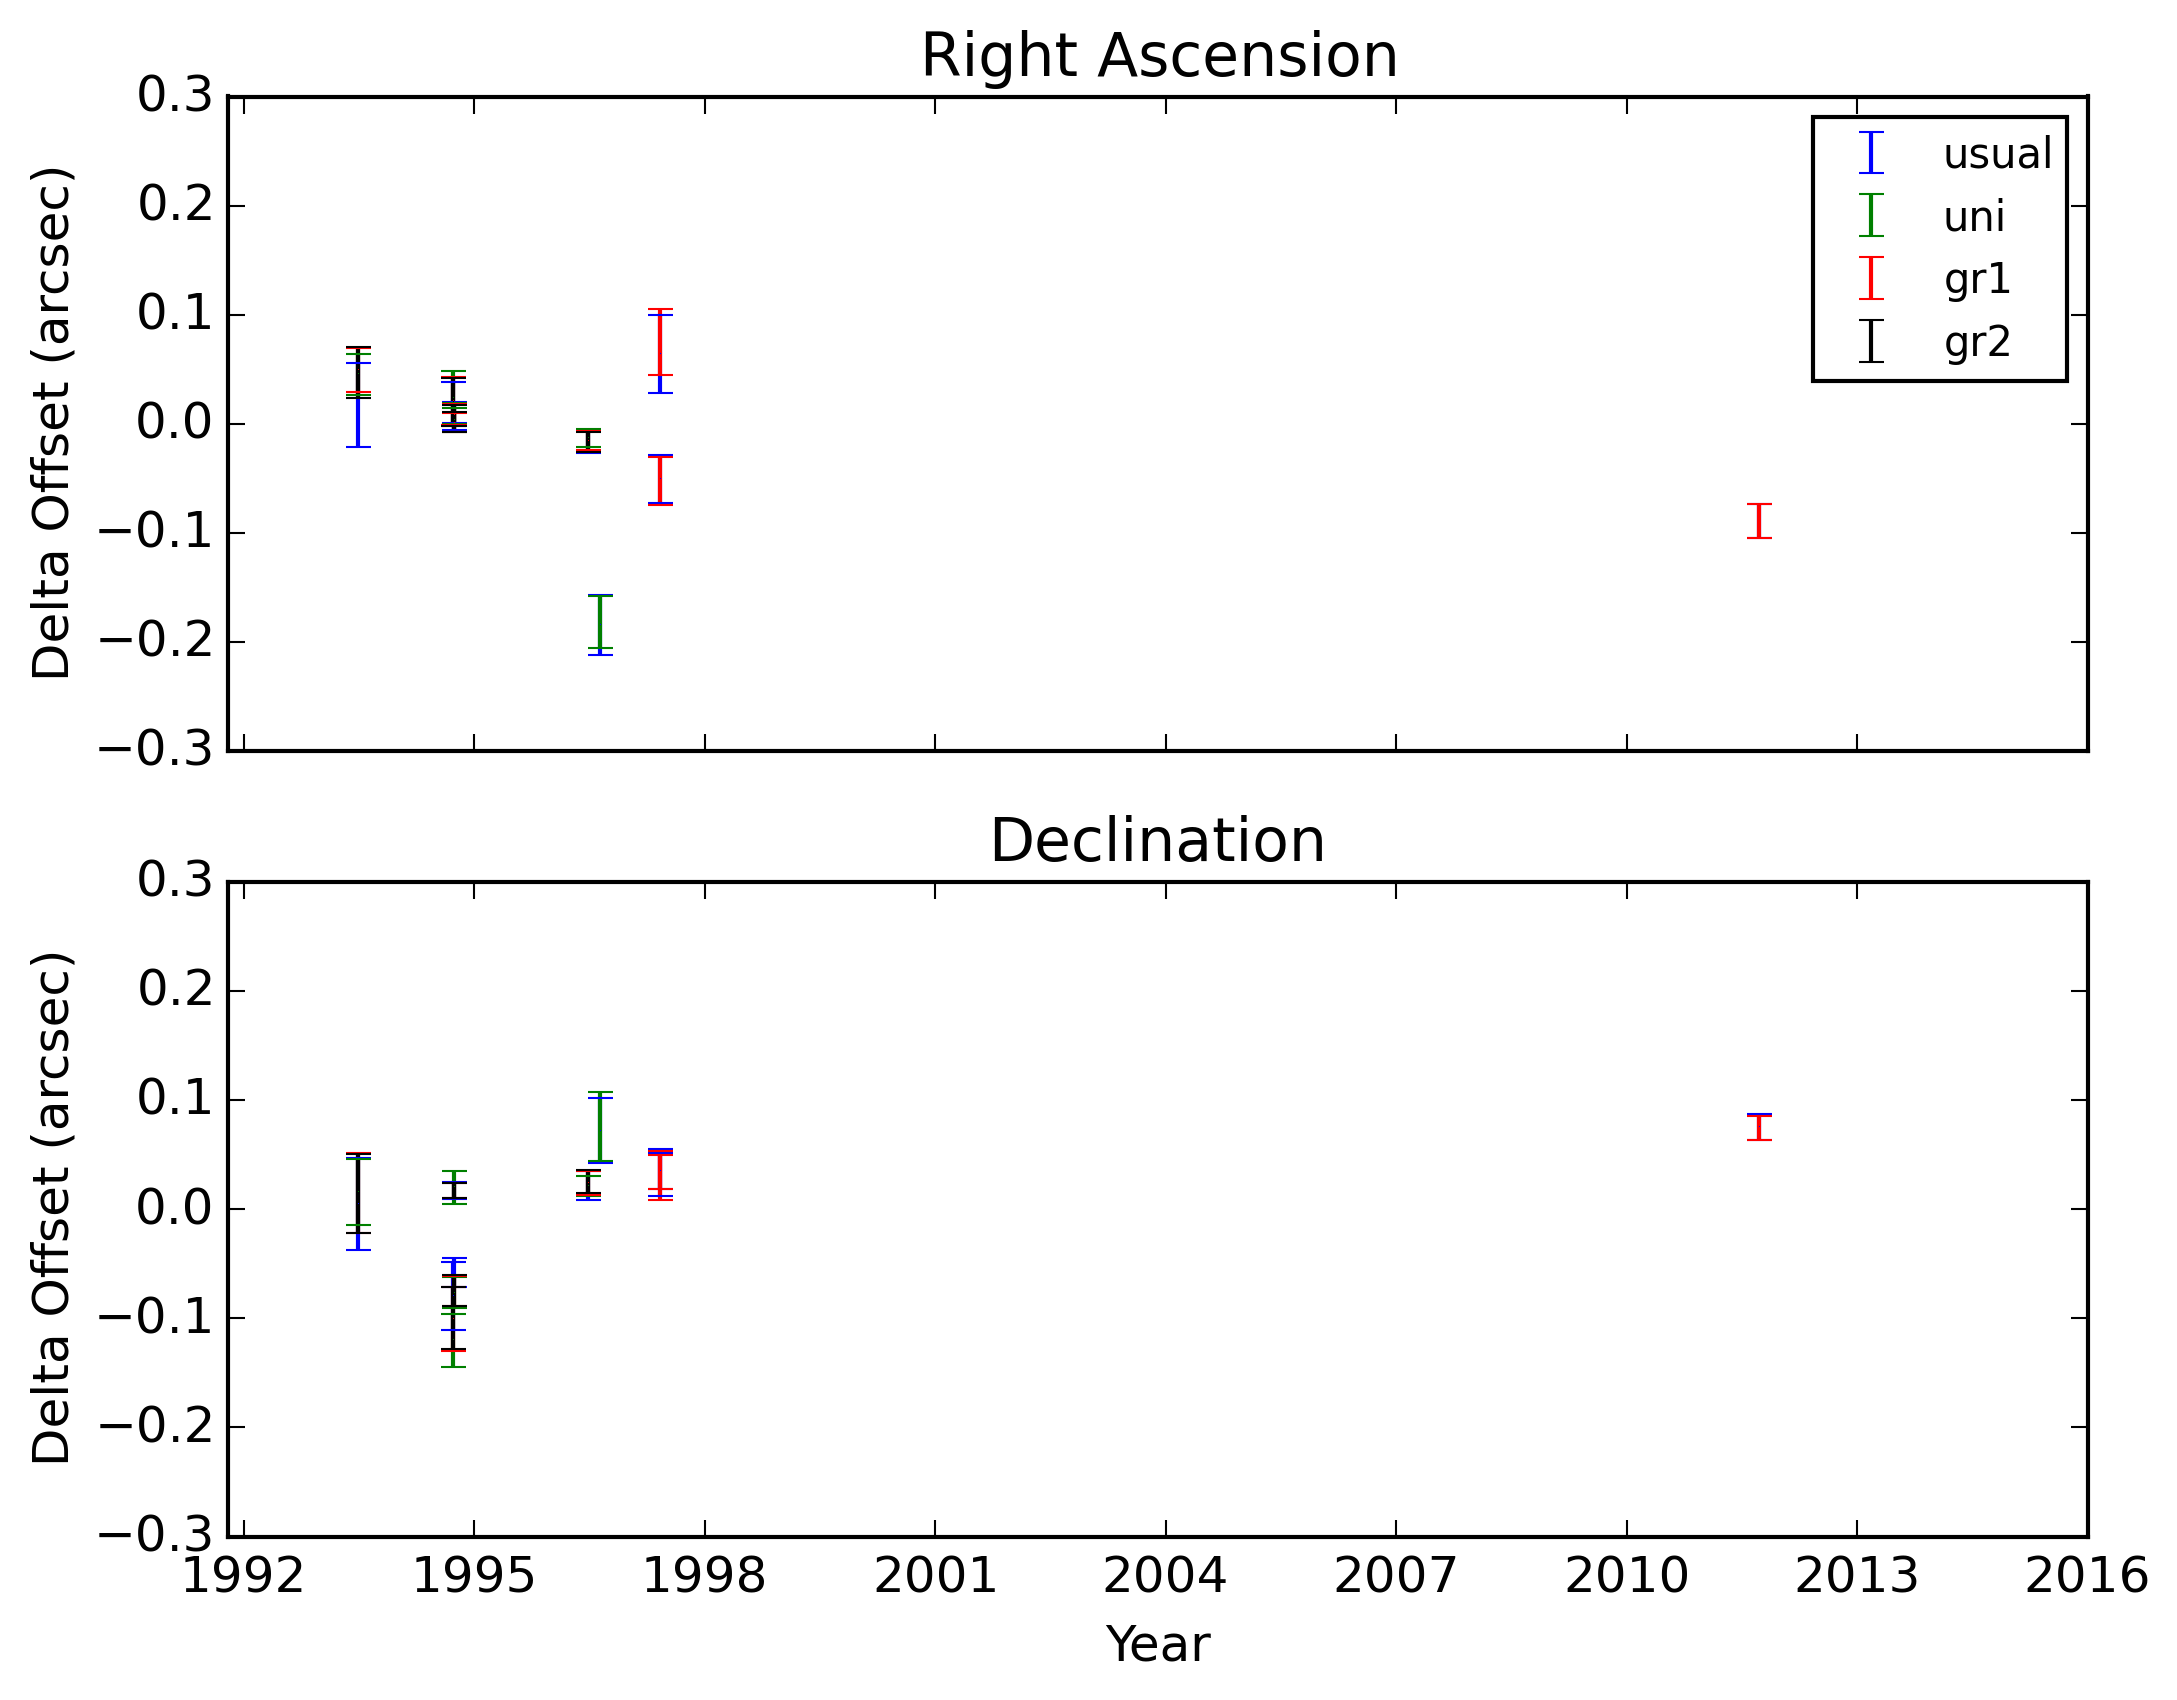
\includegraphics[width=16.0cm]{Triton-Netuno_nsat_match.png} 
%\caption{Difference between Triton's and Neptune's offsets using only positions where the two objects are in the same image. 'usual' stands for the situation 1 with the standard procedure of reduction. 'uni' stands for situation 2 with the uniform reduction. 'gr1' stands for situation 3 with global reduction over the identified stars in the procedure 1. 'gr2' stands for situation 4 with global reduction over the identified stars in the procedure 2.}
%\label{Fig:test-match}
%\end{figure}
%
%\begin{figure}
%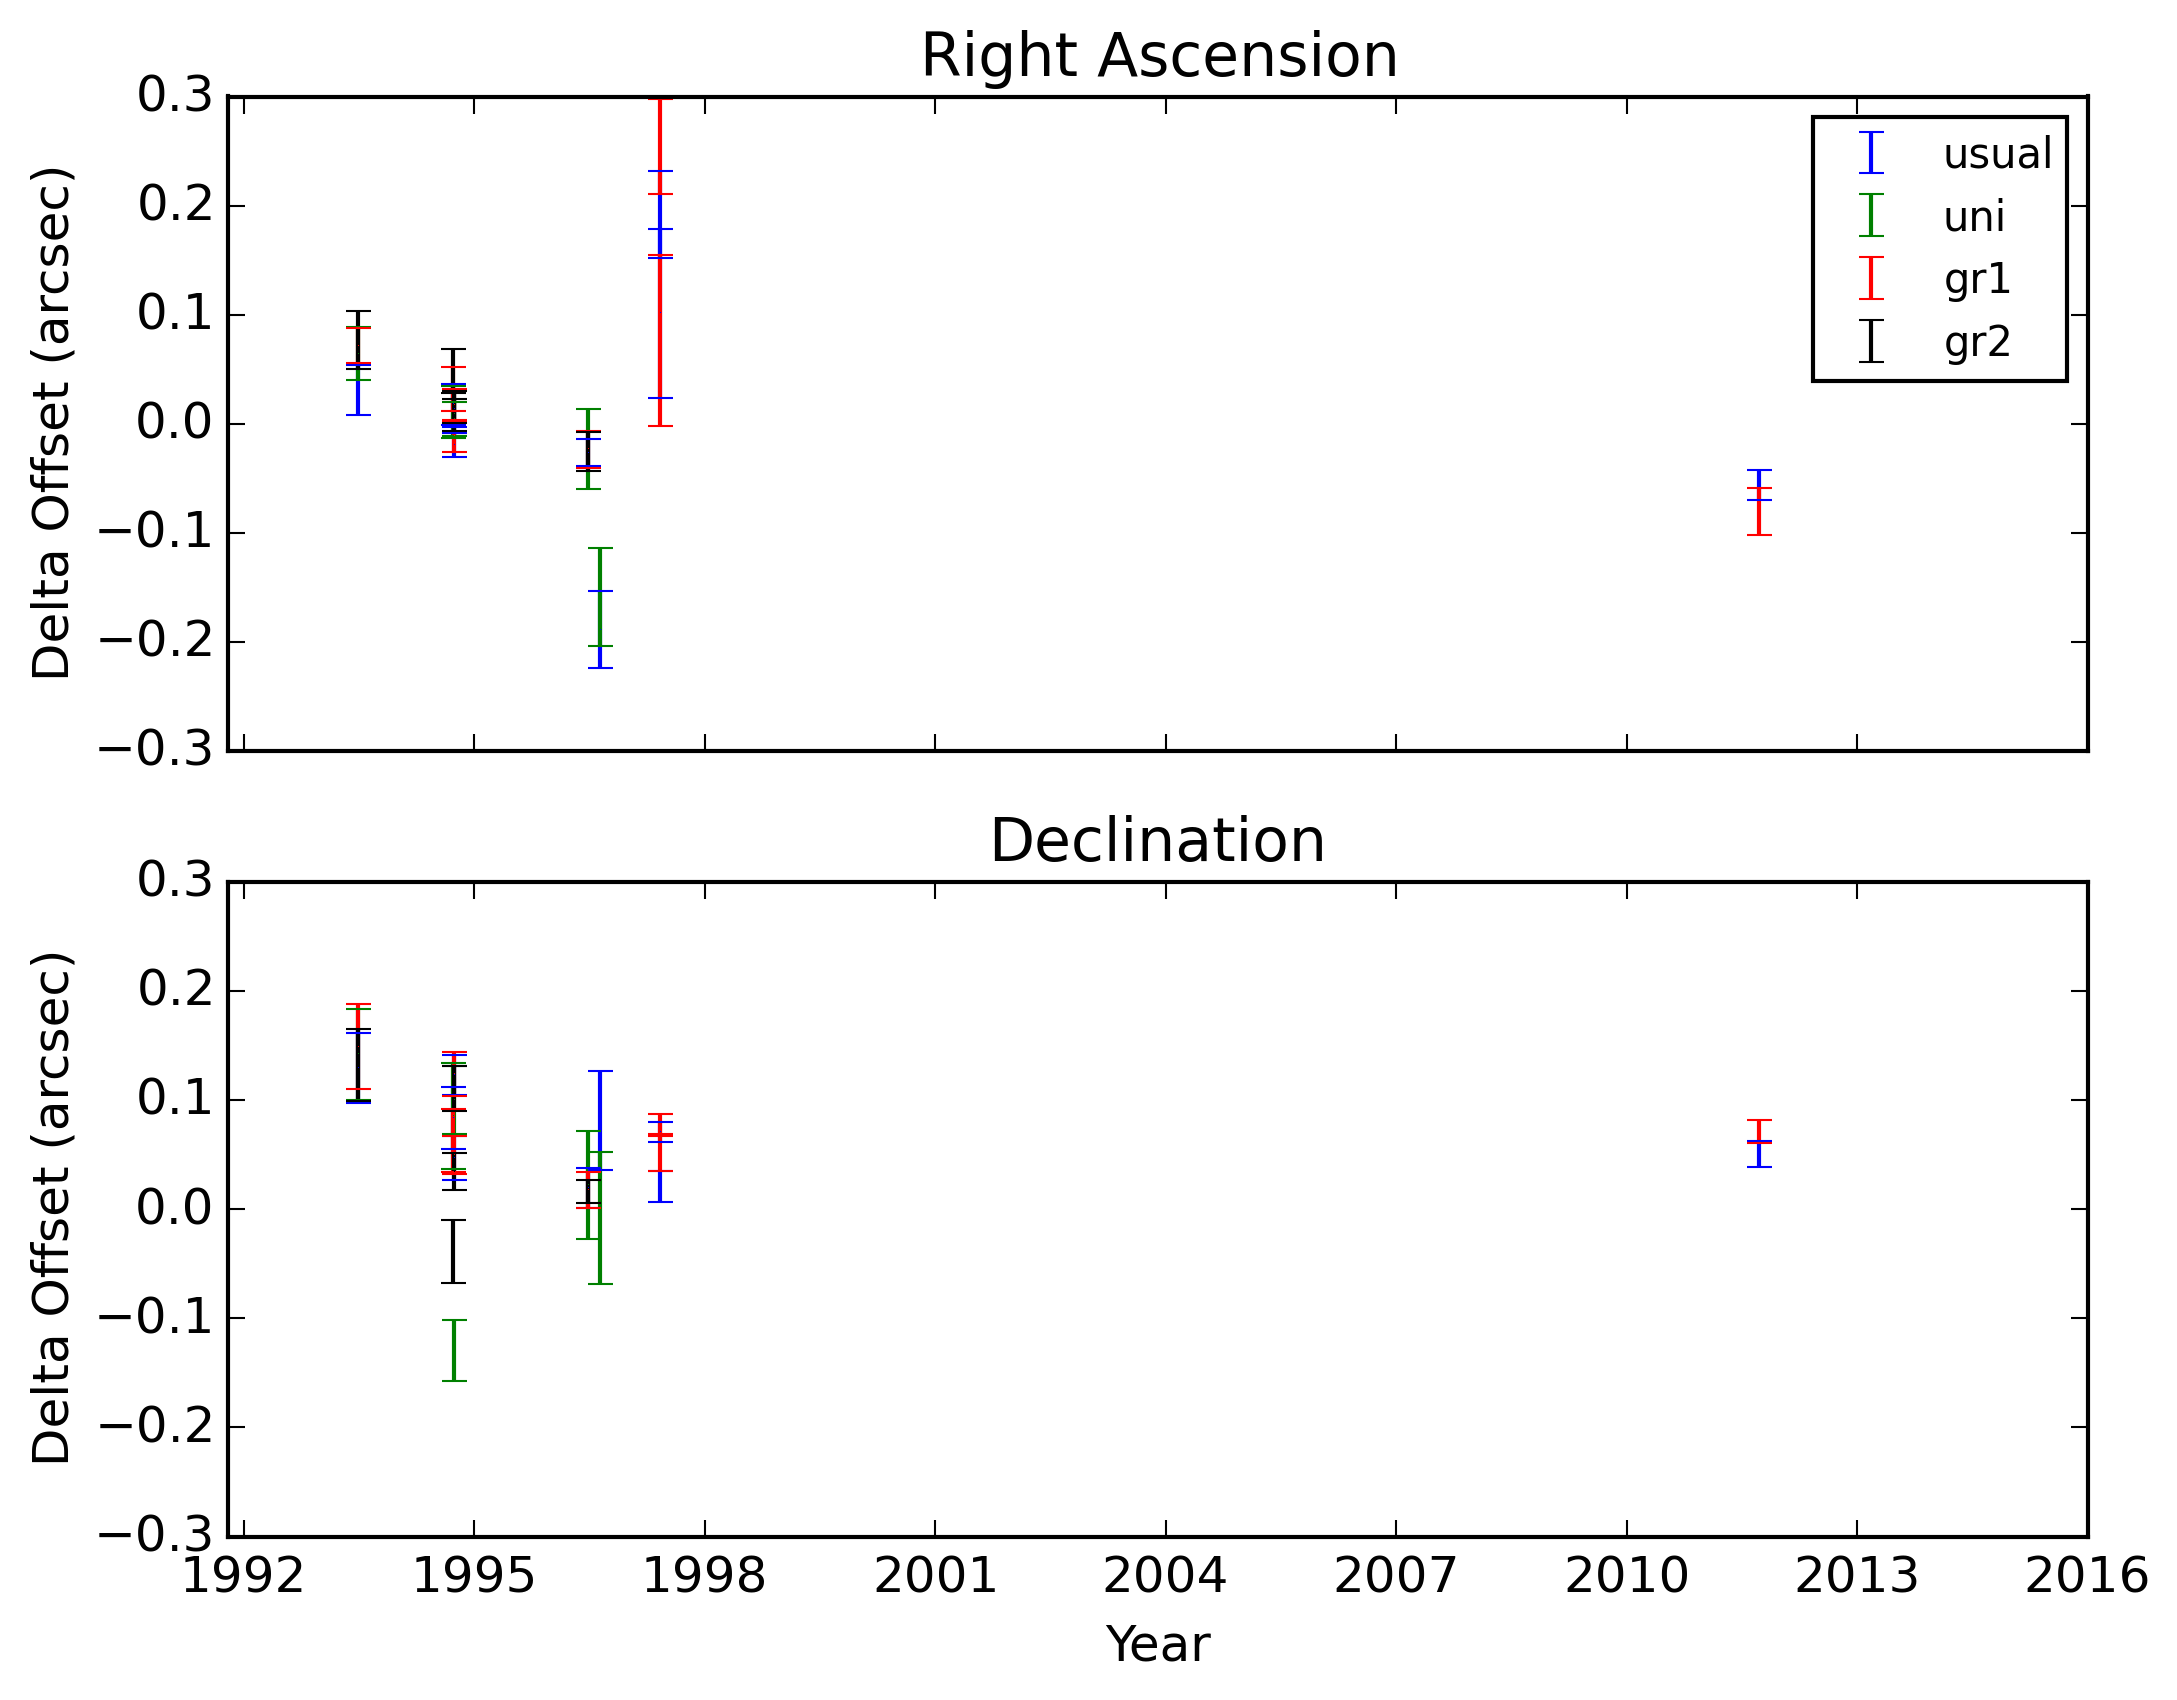
\includegraphics[width=16.0cm]{Triton-Netuno_sat.png} 
%\caption{Difference between Triton's and Neptune's offsets using the positions of Neptune in the frames with short exposure time and the positions of Triton in the frames with long exposure time (where Neptune image were saturated). Labels is the same as in Fig. \ref{Fig:test-match}}
%\label{Fig:test-sat}
%\end{figure}
%
%
%
%\begin{landscape}
%
%\begin{longtable}{|c|c|c|c|c|c|c|c|c|c|c|c|c|c|}
%\caption{Table with the data used in the Figs. \ref{Fig:test-match} and \ref{Fig:test-sat}. Situation 1 is for the positions of Triton and Neptune in the same frame. Situation 2 is for the position of Neptune in frames with short exposure time and the positions of Triton in the frames with long exposure time (where Neptune image were saturated). 'Usual' stands for the situation 1 with the standard procedure of reduction. 'Uni' stands for situation 2 with the uniform reduction. 'GR1' stands for situation 3 with global reduction over the identified stars in the procedure 1. 'GR2' stands for situation 4 with global reduction over the identified stars in the procedure 2. N is the number of positions used. For the situation 2 N is not presented because there may have different numbers of positions for Triton and Neptune used. For some nights, the uniform or global reduction procedure had issues, so they are not presented.}\\
%\hline
%Night & Sit & \multicolumn{3}{|c|}{Usual} & \multicolumn{3}{|c|}{Uni} & \multicolumn{3}{|c|}{GR1} & \multicolumn{3}{|c|}{GR2} \\
%%\hline
% & &  RA & DEC & N & RA & DEC & N & RA & DEC & N & RA & DEC & N \\
%\hline
%\endfirsthead
%\multicolumn{13}{c}%
%{\tablename\ \thetable\ -- \textit{Continued from previous page}} \\
%\hline
%Night & Sit & \multicolumn{3}{|c|}{Usual} & \multicolumn{3}{|c|}{Uni} & \multicolumn{3}{|c|}{GR1} & \multicolumn{3}{|c|}{GR2} \\
%%\hline
% & &  RA & DEC & N & RA & DEC & N & RA & DEC & N & RA & DEC & N \\
%\hline
%\endhead
%\hline \multicolumn{13}{r}{\textit{Continued on next page}} \\
%\endfoot
%\hline
%\endlastfoot
%1993-06-23 & 1 & 17 $\pm$ 38 & 5 $\pm$ 42 & 9 & 45 $\pm$ 18 & 15 $\pm$ 30 & 5 & 49 $\pm$ 20 & 15 $\pm$ 36 & 7 & 47 $\pm$ 23 & 14 $\pm$ 36 & 7\\
% & 2 & 30 $\pm$ 22 & 129 $\pm$ 32 & - & 64 $\pm$ 23 & 142 $\pm$ 41 & - & 71 $\pm$ 16 & 149 $\pm$ 39 & - & 76 $\pm$ 26 & 132 $\pm$ 32 & - \\
%\hline
%
%1994-09-22 & 1 & 18 $\pm$ 20 & -79 $\pm$ 31 & 10 & 23 $\pm$ 24 & -12 $\pm$ 24 & 6 & 20 $\pm$ 22 & -100 $\pm$ 29 & 10 & 20 $\pm$ 22 & -99 $\pm$ 28 & 10\\
% & 2 &  17 $\pm$ 19 & 83 $\pm$ 28 & - & 10 $\pm$ 24 & 85 $\pm$ 48 & - & 31 $\pm$ 20 & 62 $\pm$ 28 & - & 48 $\pm$ 20 & -38 $\pm$ 28 & -\\
%\hline
%
%1994-09-23 & 1 & 7 $\pm$ 13 & -57 $\pm$ 13 & 10 & 9 $\pm$ 9 & -76 $\pm$ 14 & 9 & 8 $\pm$ 9 & -75 $\pm$ 14 & 9 & 7 $\pm$ 9 & -75 $\pm$ 14 & 9\\
% & 2 & 13 $\pm$ 16 & 47 $\pm$ 20 & - & 9 $\pm$ 20 & -129 $\pm$ 27 & - & 17 $\pm$ 14 & 49 $\pm$ 17 & - & 15 $\pm$ 14 & 34 $\pm$ 16 & -\\
%\hline
%
%1994-09-24 & 1 & -28 $\pm$ 4 & 17 $\pm$ 8 & 5 & 3 $\pm$ 10 & 20 $\pm$ 14 & 9 & 1 $\pm$ 9 & 17 $\pm$ 6 & 6 & 1 $\pm$ 8 & 17 $\pm$ 7 & 6\\
% & 2 & -19 $\pm$ 11 &  123 $\pm$ 18 & - & 4 $\pm$ 15 &  99 $\pm$ 31 & - & -11 $\pm$ 14 &  123 $\pm$ 20 & - & 7 $\pm$ 14 & 110 $\pm$ 20 & -\\
%\hline
%
%1996-06-22 & 1 & -16 $\pm$ 10 & 21 $\pm$ 13 & 9 & -12 $\pm$ 8 & 21 $\pm$ 9 & 8 & -15 $\pm$ 8 & 24 $\pm$ 10 & 8 & -16 $\pm$ 9 & 25 $\pm$ 10 & 8\\
% & 2 & -26 $\pm$ 12 & 19 $\pm$ 18 & - & -22 $\pm$ 36 & 22 $\pm$ 49 & - & -23 $\pm$ 16 & 17 $\pm$ 16 & - & -25 $\pm$ 17 & 15 $\pm$ 10 & -\\
%\hline
%
%1996-08-21 & 1 & -184 $\pm$ 27 & 72 $\pm$ 29 & 13 & -181 $\pm$ 24 & 76 $\pm$ 31 & 13 & - & - & - & - & - & - \\
% & 2 & -188 $\pm$ 35 &  81 $\pm$ 45 & - & -159 $\pm$ 44 & -8 $\pm$ 60 & - & - & - & - & - & - & -\\
%\hline
%
%1997-06-01 & 1 & -50 $\pm$ 21 & 34 $\pm$ 16 & 26 & - & - & - & -52 $\pm$ 21 & 34 $\pm$ 15 & 26 & - & - & -\\
% & 2 & 191 $\pm$ 39 &  70 $\pm$ 9 & - & - & - & - & 254 $\pm$ 43 &  77 $\pm$ 9 & - & - & - & -\\
%\hline
%
%1997-06-02 & 1 & 6 $\pm$ 35 & 33 $\pm$ 21 & 22 & - & - & - & 75 $\pm$ 30 & 30 $\pm$ 22 & 19 & - & - & -\\
% & 2 & 101 $\pm$ 77 &  20 $\pm$ 14 & - & - & - & - & 76 $\pm$ 78 & 52 $\pm$ 16 & - & - & - & -\\
%\hline
%
%2011-09-19 & 1 & -88 $\pm$ 15 & 75 $\pm$ 12 & 35 & - & - & - & -88 $\pm$ 15 & 74 $\pm$ 11 & 35 & - & - & -\\
% & 2 & -55 $\pm$ 13 & 50 $\pm$ 11 & - & - & - & - & -80 $\pm$ 21 & 71 $\pm$ 10 & - & - & - & -\\
%\hline
%
%\hline
%\end{longtable}
%
%\end{landscape}

\section*{Chromatic Refraction Test}

Table \ref{Tab:colors} shows the colors for Triton \citep{Pascu2006} and Neptune \cite{Schmude2016}. Their colors are very different in the blue region. So it is expected that their positions have influence of chromatic refraction with different intensities. The apparent position of Neptune, which is more blue than Triton, would be more shifted towards the zenith than the Triton's position. There may also be noted that in 1992 Neptune had just exited the galactic plane, so the reference stars were redder due to dust.

\begin{table*}[h]
\centering
\begin{tabular}{|l|c|c|c|c|c|}
\hline
Object & U-B & B-V & V-R & R-I & V-I\\
\hline
Triton (leading side) & & +0.696$\pm$0.009 & & & +0.766$\pm$0.006 \\
Triton (trailing side) & & +0.699$\pm$0.006 & & & +0.776$\pm$0.007 \\
Neptune & +0.14 & +0.39 & -0.29 & -1.05 & +0.76*\\
\hline
\end{tabular}
\caption{Colors of Triton and Neptune. Leading side is the hemisphere of Triton that is in the direction of its movement. Trailing side is the opposite hemisphere. *calculated from V-R and R-I colors.}
\label{Tab:colors}
\end{table*}

To test the effects of chromatic refraction I used the method of \cite{Benedetti-Rossi2014} on all nights with observations distributed over more than 1.5h of hour angle. I used the equation \:
\begin{equation}
\Delta [\alpha, \delta] = V_{\alpha,\delta} (\phi,\delta, H) \cdot \Delta B,
\label{Eq:refraction}
\end{equation}
to model the chromatic refraction of the nights. $\Delta [\alpha, \delta]$ is the position offset for each coordinate ($\alpha, \delta$), $V_{\alpha,\delta} (\phi,\delta, H)$ is the first part of refraction which is due to the position of the observed objects and is a function of the latitude of the site ($\phi$), of the object’s declination ($\delta$), and of the hour angle ($H$) and $\Delta B$ is the the second part: the differential chromatic refraction which is due to the atmospheric conditions and the wavelength ($\lambda$) of the object and of the stars in the field. This equation is available in \cite{Benedetti-Rossi2014} where it was applied for observations of Pluto.

Figs. \ref{Fig:refraction-net-160}-\ref{Fig:refraction-tri-iag} show the distributions of the offsets in RA and DEC before and after the elimination of chromatic refraction (Neptune-160, Triton-160, Neptune-IAG, Triton-IAG, respectively). Only nights with $\Delta H > 1.5h$. The histograms clearly show an improvement in the distribution of the offsets, mainly for Neptune. So chromatic refraction is very important and must be removed. % looked for nights with many observations distributed over the night. I selected five of them (\PE: 1997-05-31 and 1997-06-01; \BC: 2003-07-27, 2004-08-22 and 2011-09-25) with more than 4 hours between the first and last observations. In the nights of \PE and in the 2003 night of \BC it was used no filter (clear). In the night of 2004 it was used a filter called "Dark" which we suppose it means no filter, however we are no sure so I classified it as unknown. In the night of 2011 it was used a I filter.% In both nights there was only one exposure time used.

%In Fig \ref{Fig:refraction} it is plotted the difference in the positions of Triton and Neptune compared to the difference of their ephemeris in RA and DEC for the 5 nights.

\begin{figure}[h]
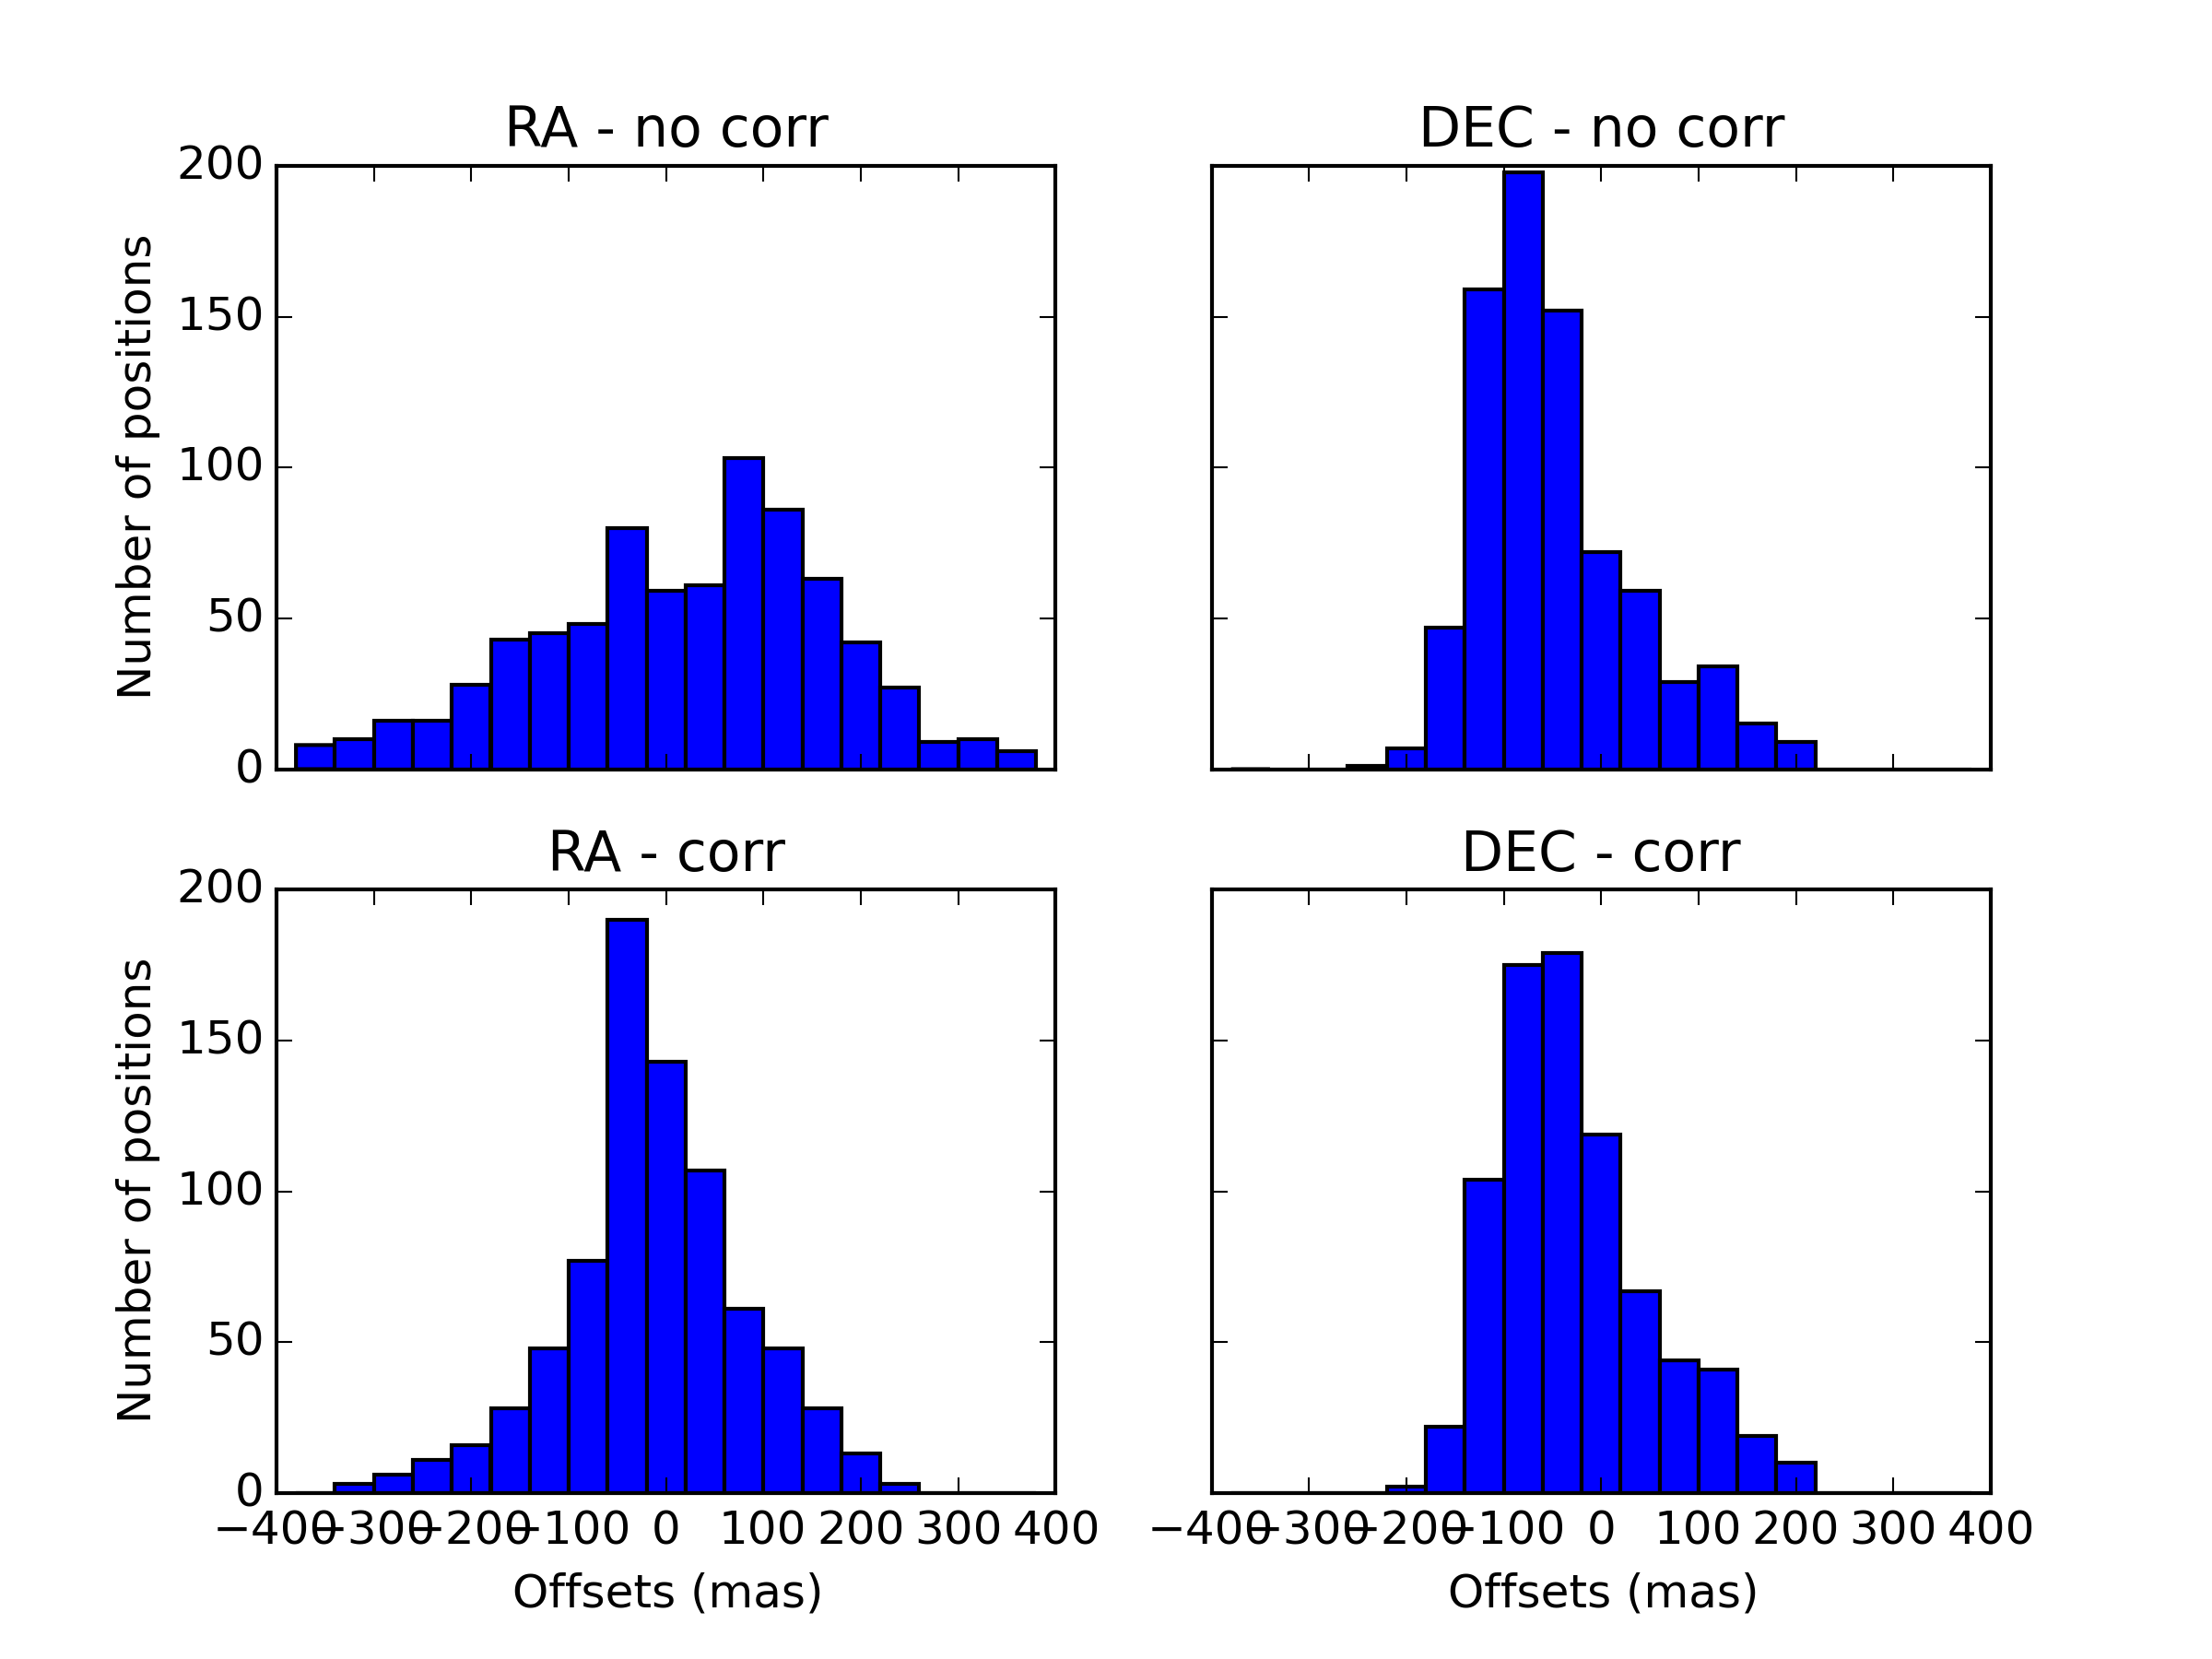
\includegraphics[width=17.0cm]{dist_Netuno_160.png} 
\caption{Distribution of the offsets of Neptune observed in 160.}
\label{Fig:refraction-net-160}
\end{figure}
\begin{figure}[h]
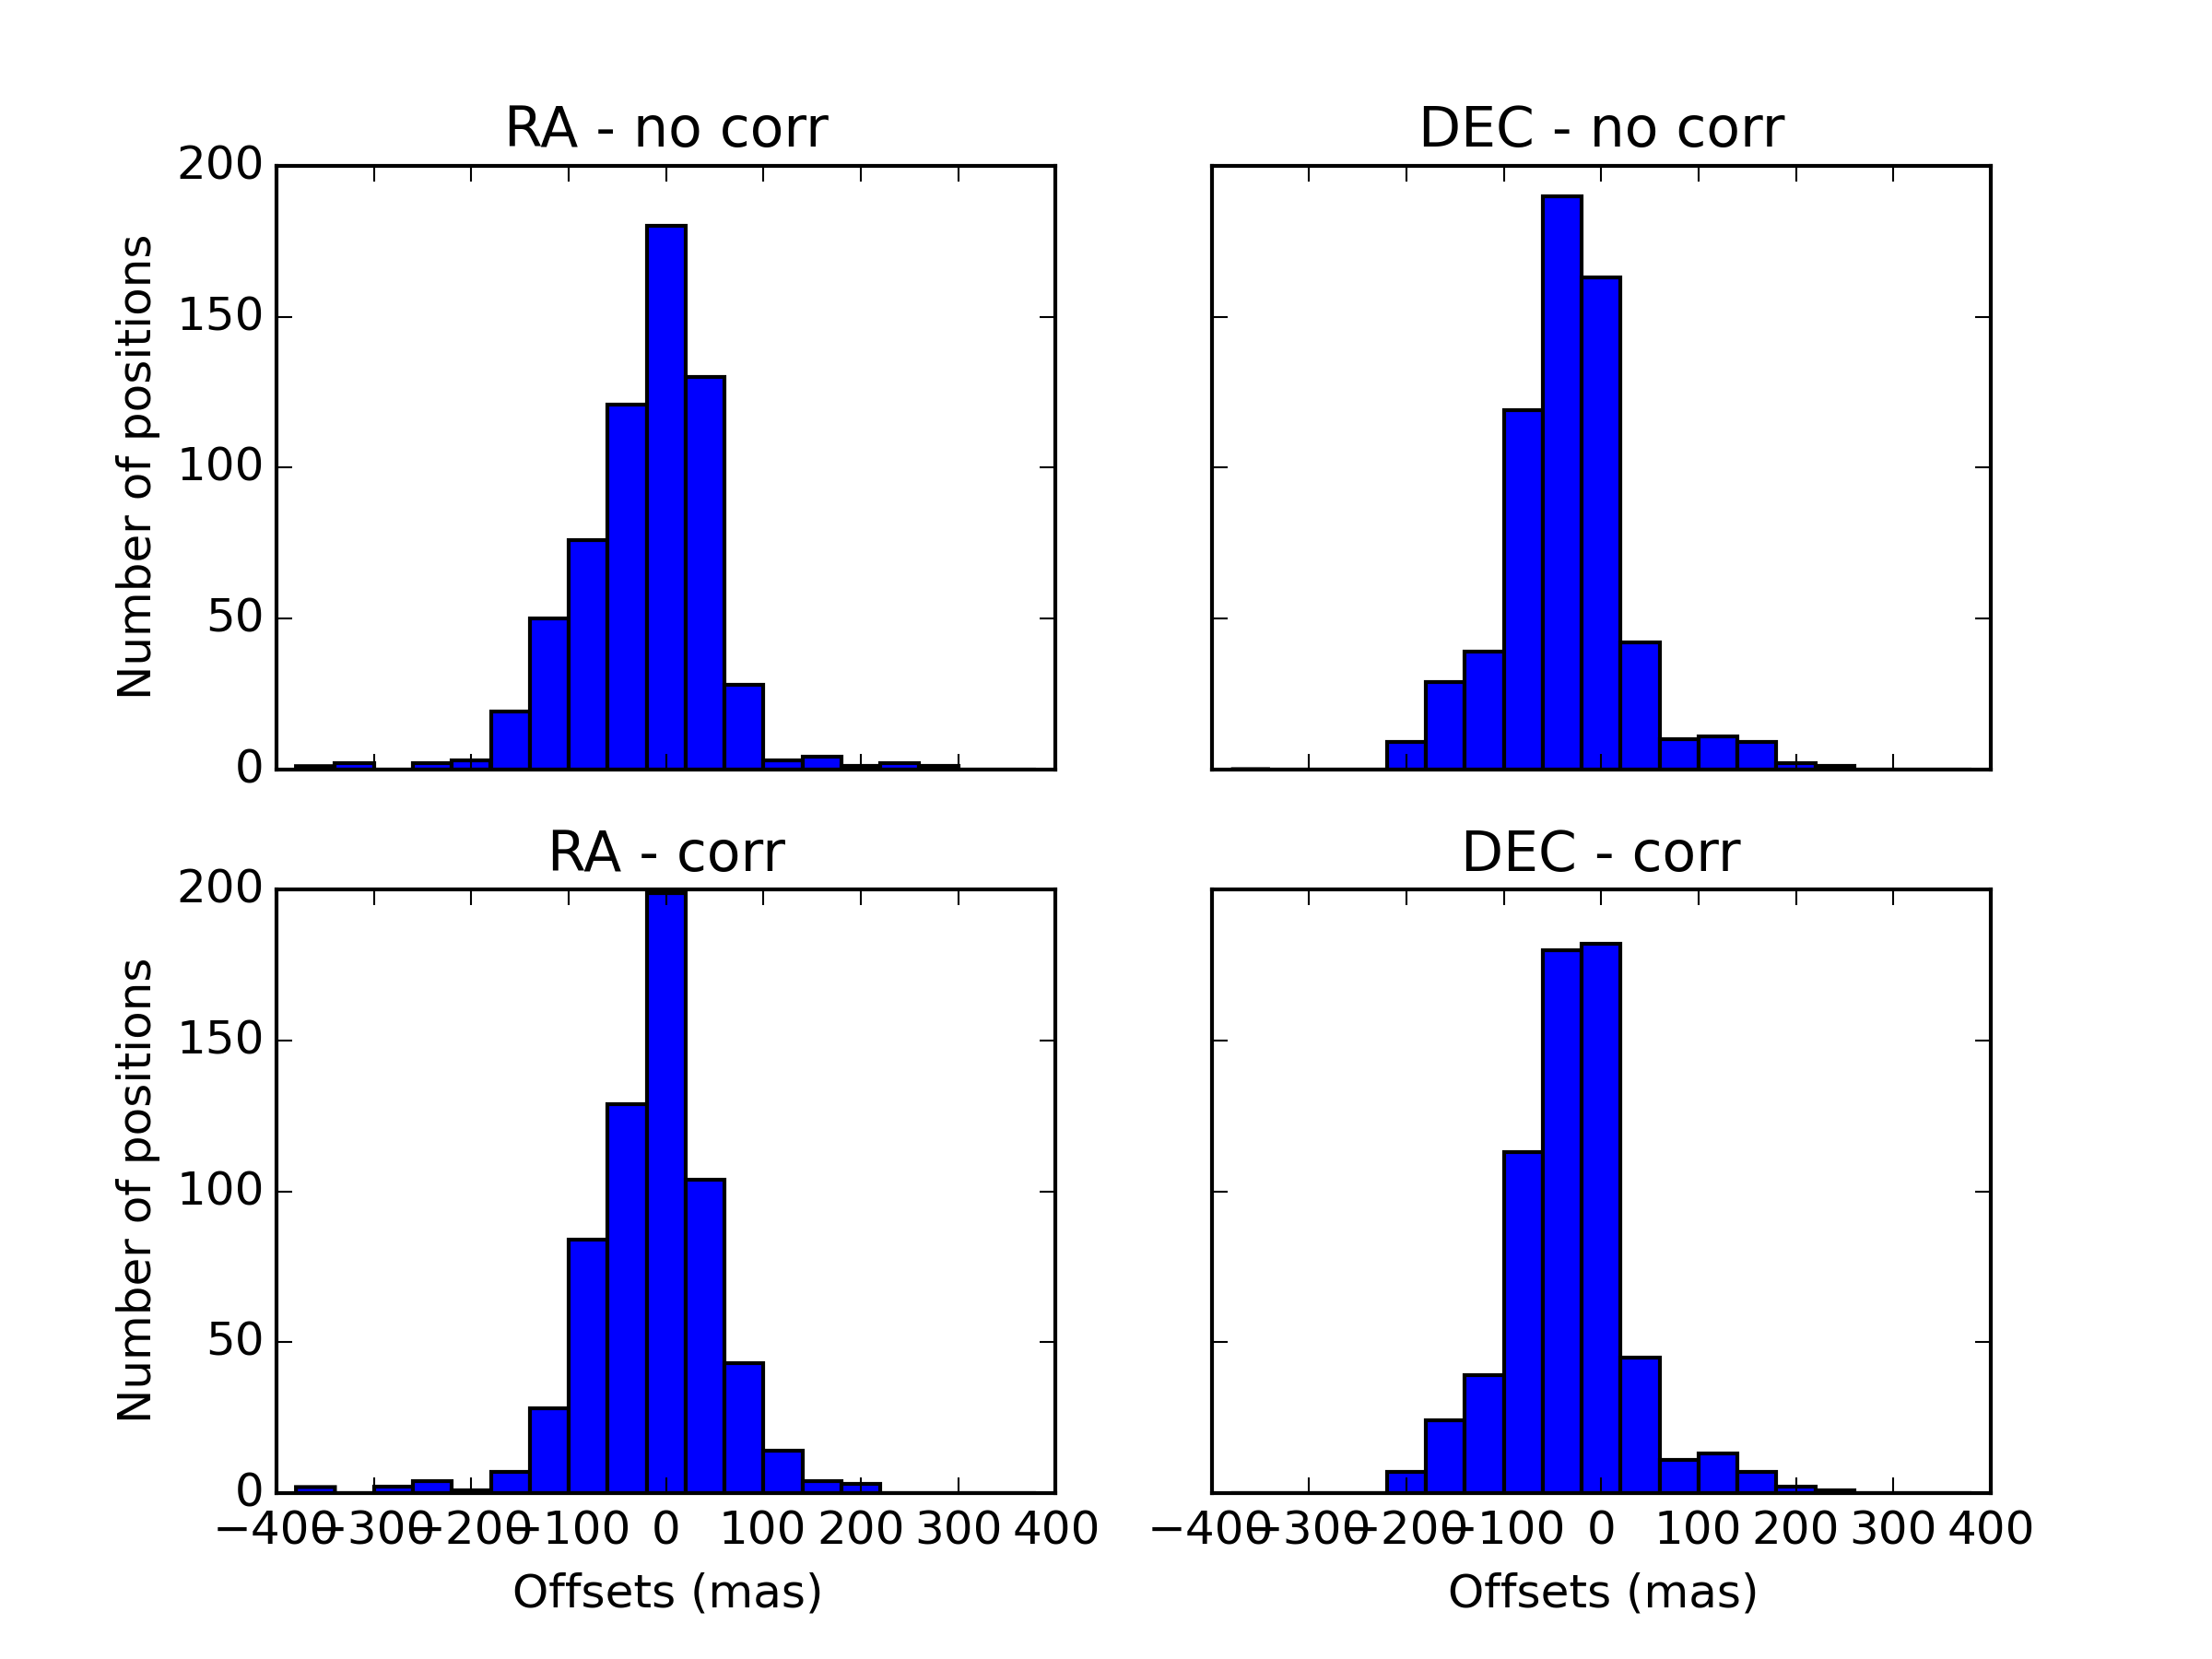
\includegraphics[width=17.0cm]{dist_Triton_160.png} 
\caption{Distribution of the offsets of Triton observed in 160.}
\label{Fig:refraction-tri-160}
\end{figure}
\begin{figure}[h]
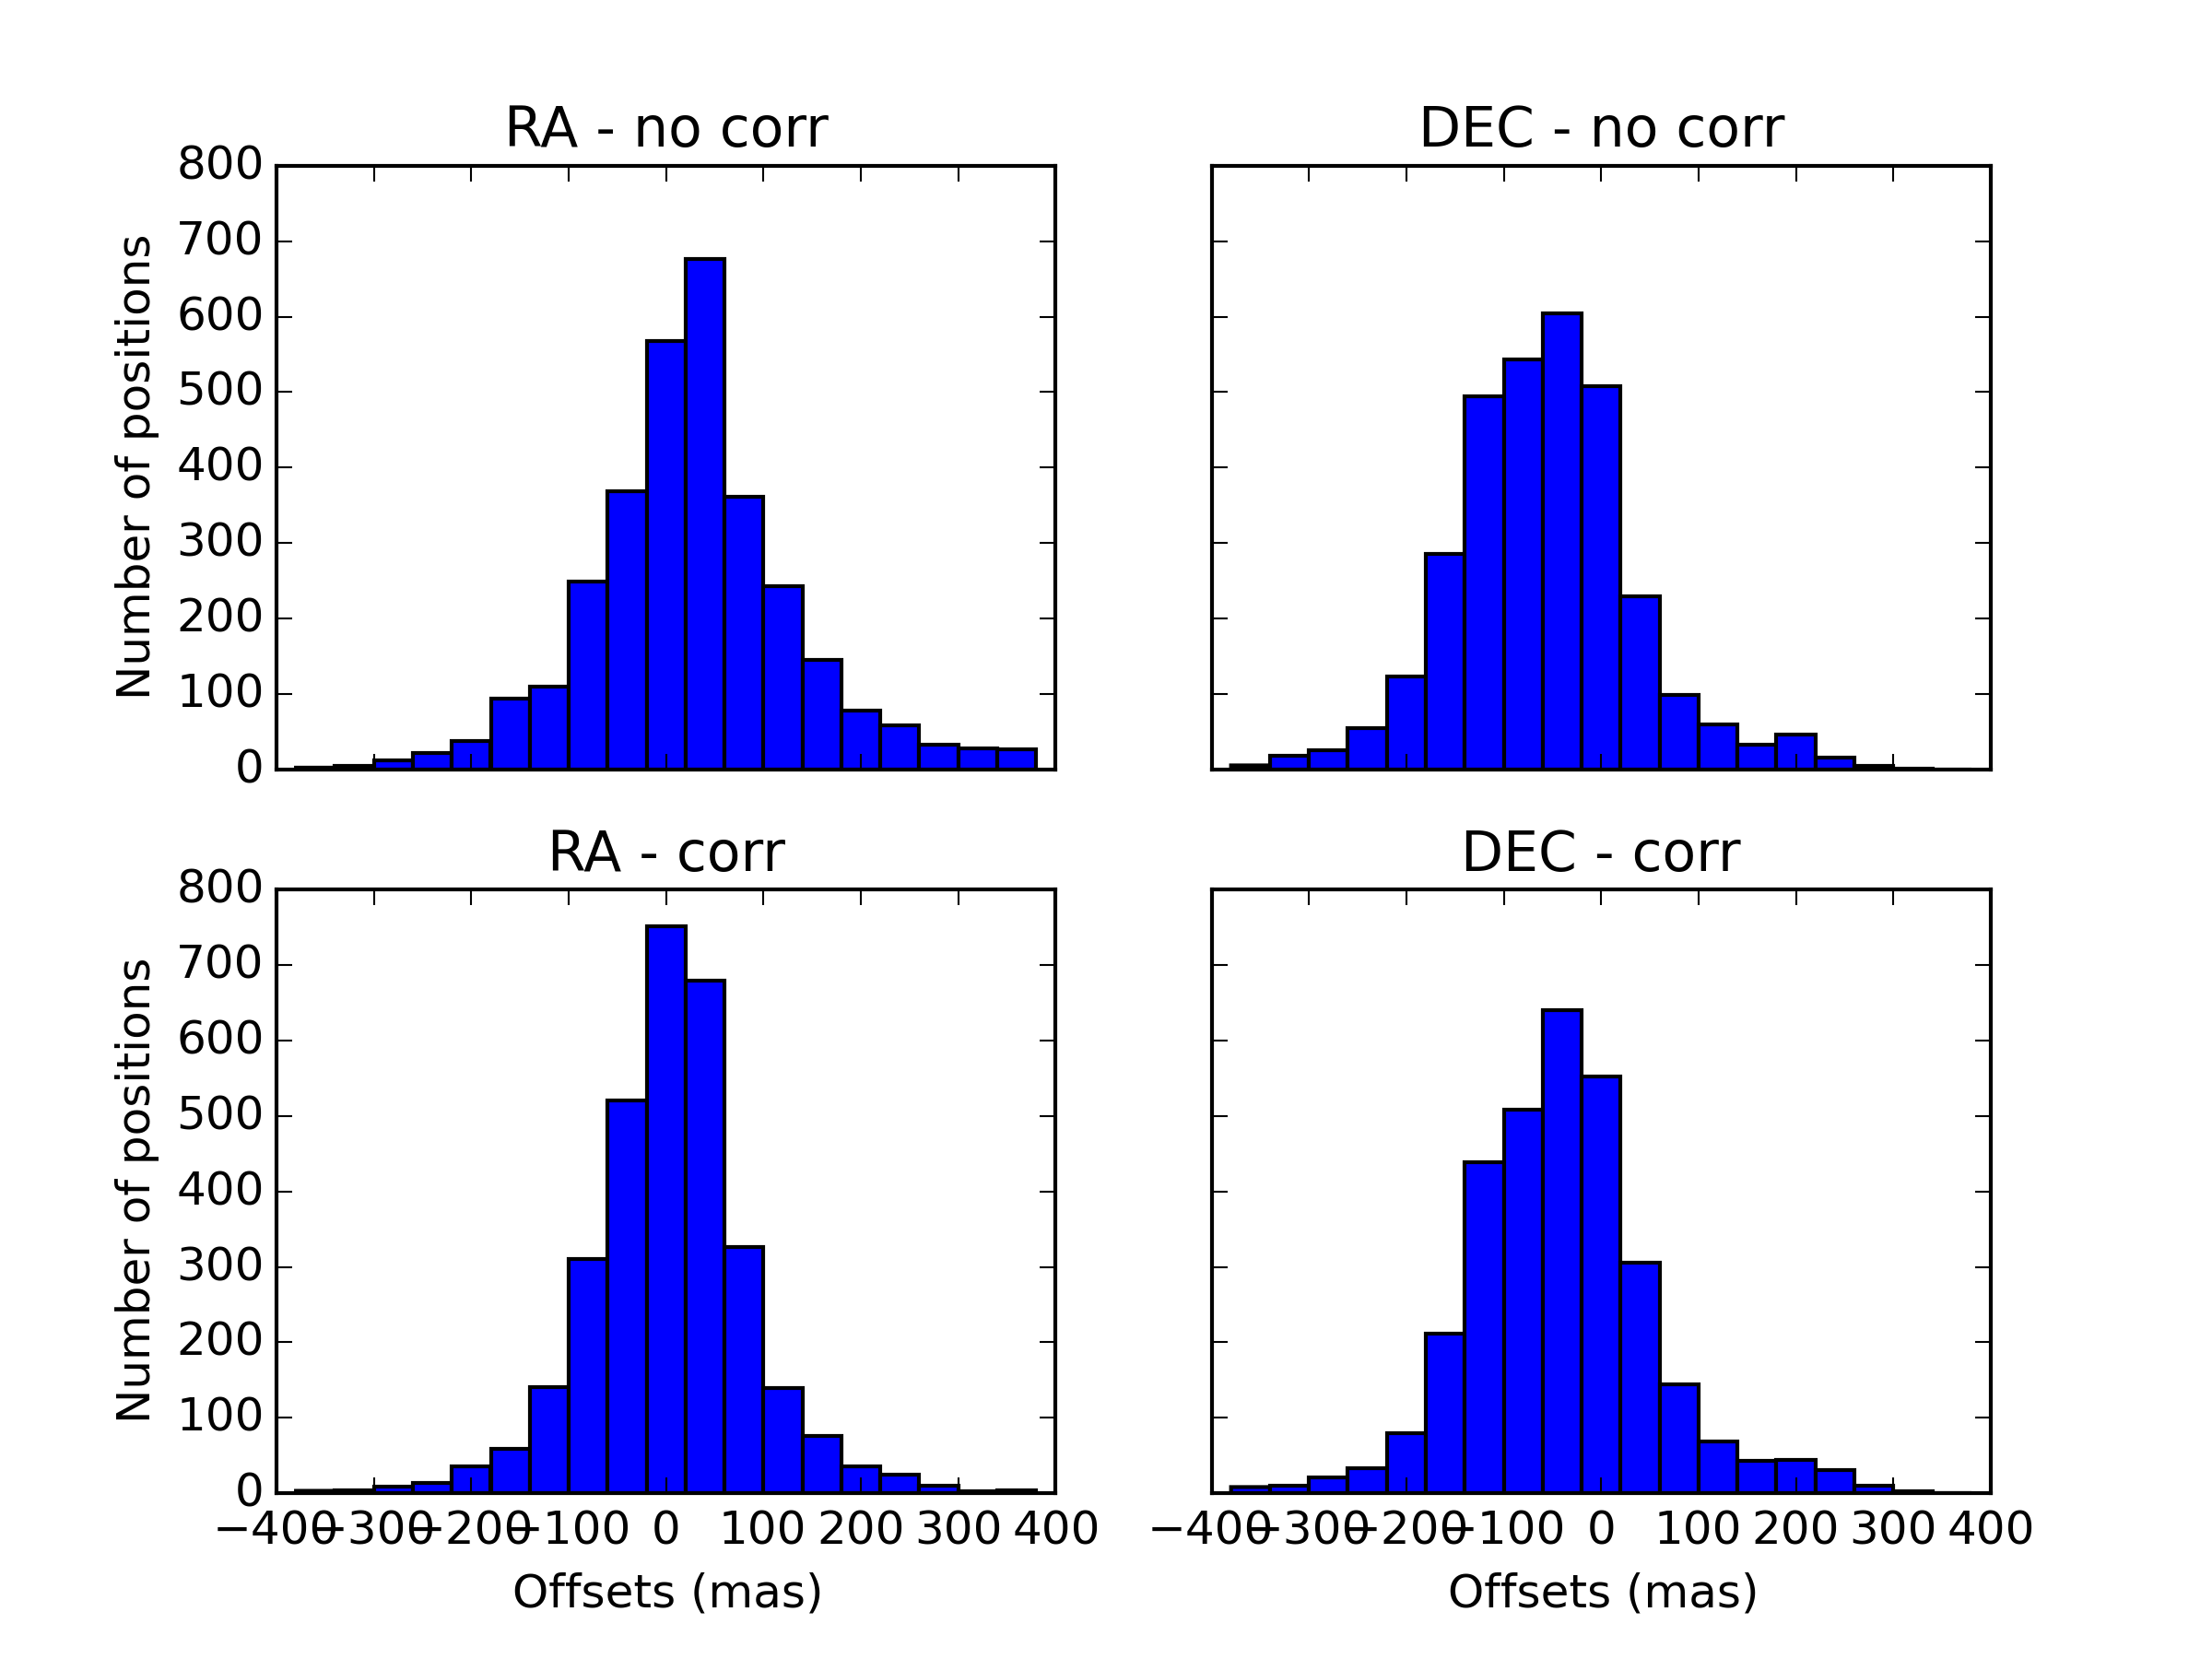
\includegraphics[width=17.0cm]{dist_Netuno_IAG.png} 
\caption{Distribution of the offsets of Neptune observed in IAG.}
\label{Fig:refraction-net-iag}
\end{figure}
\begin{figure}[h]
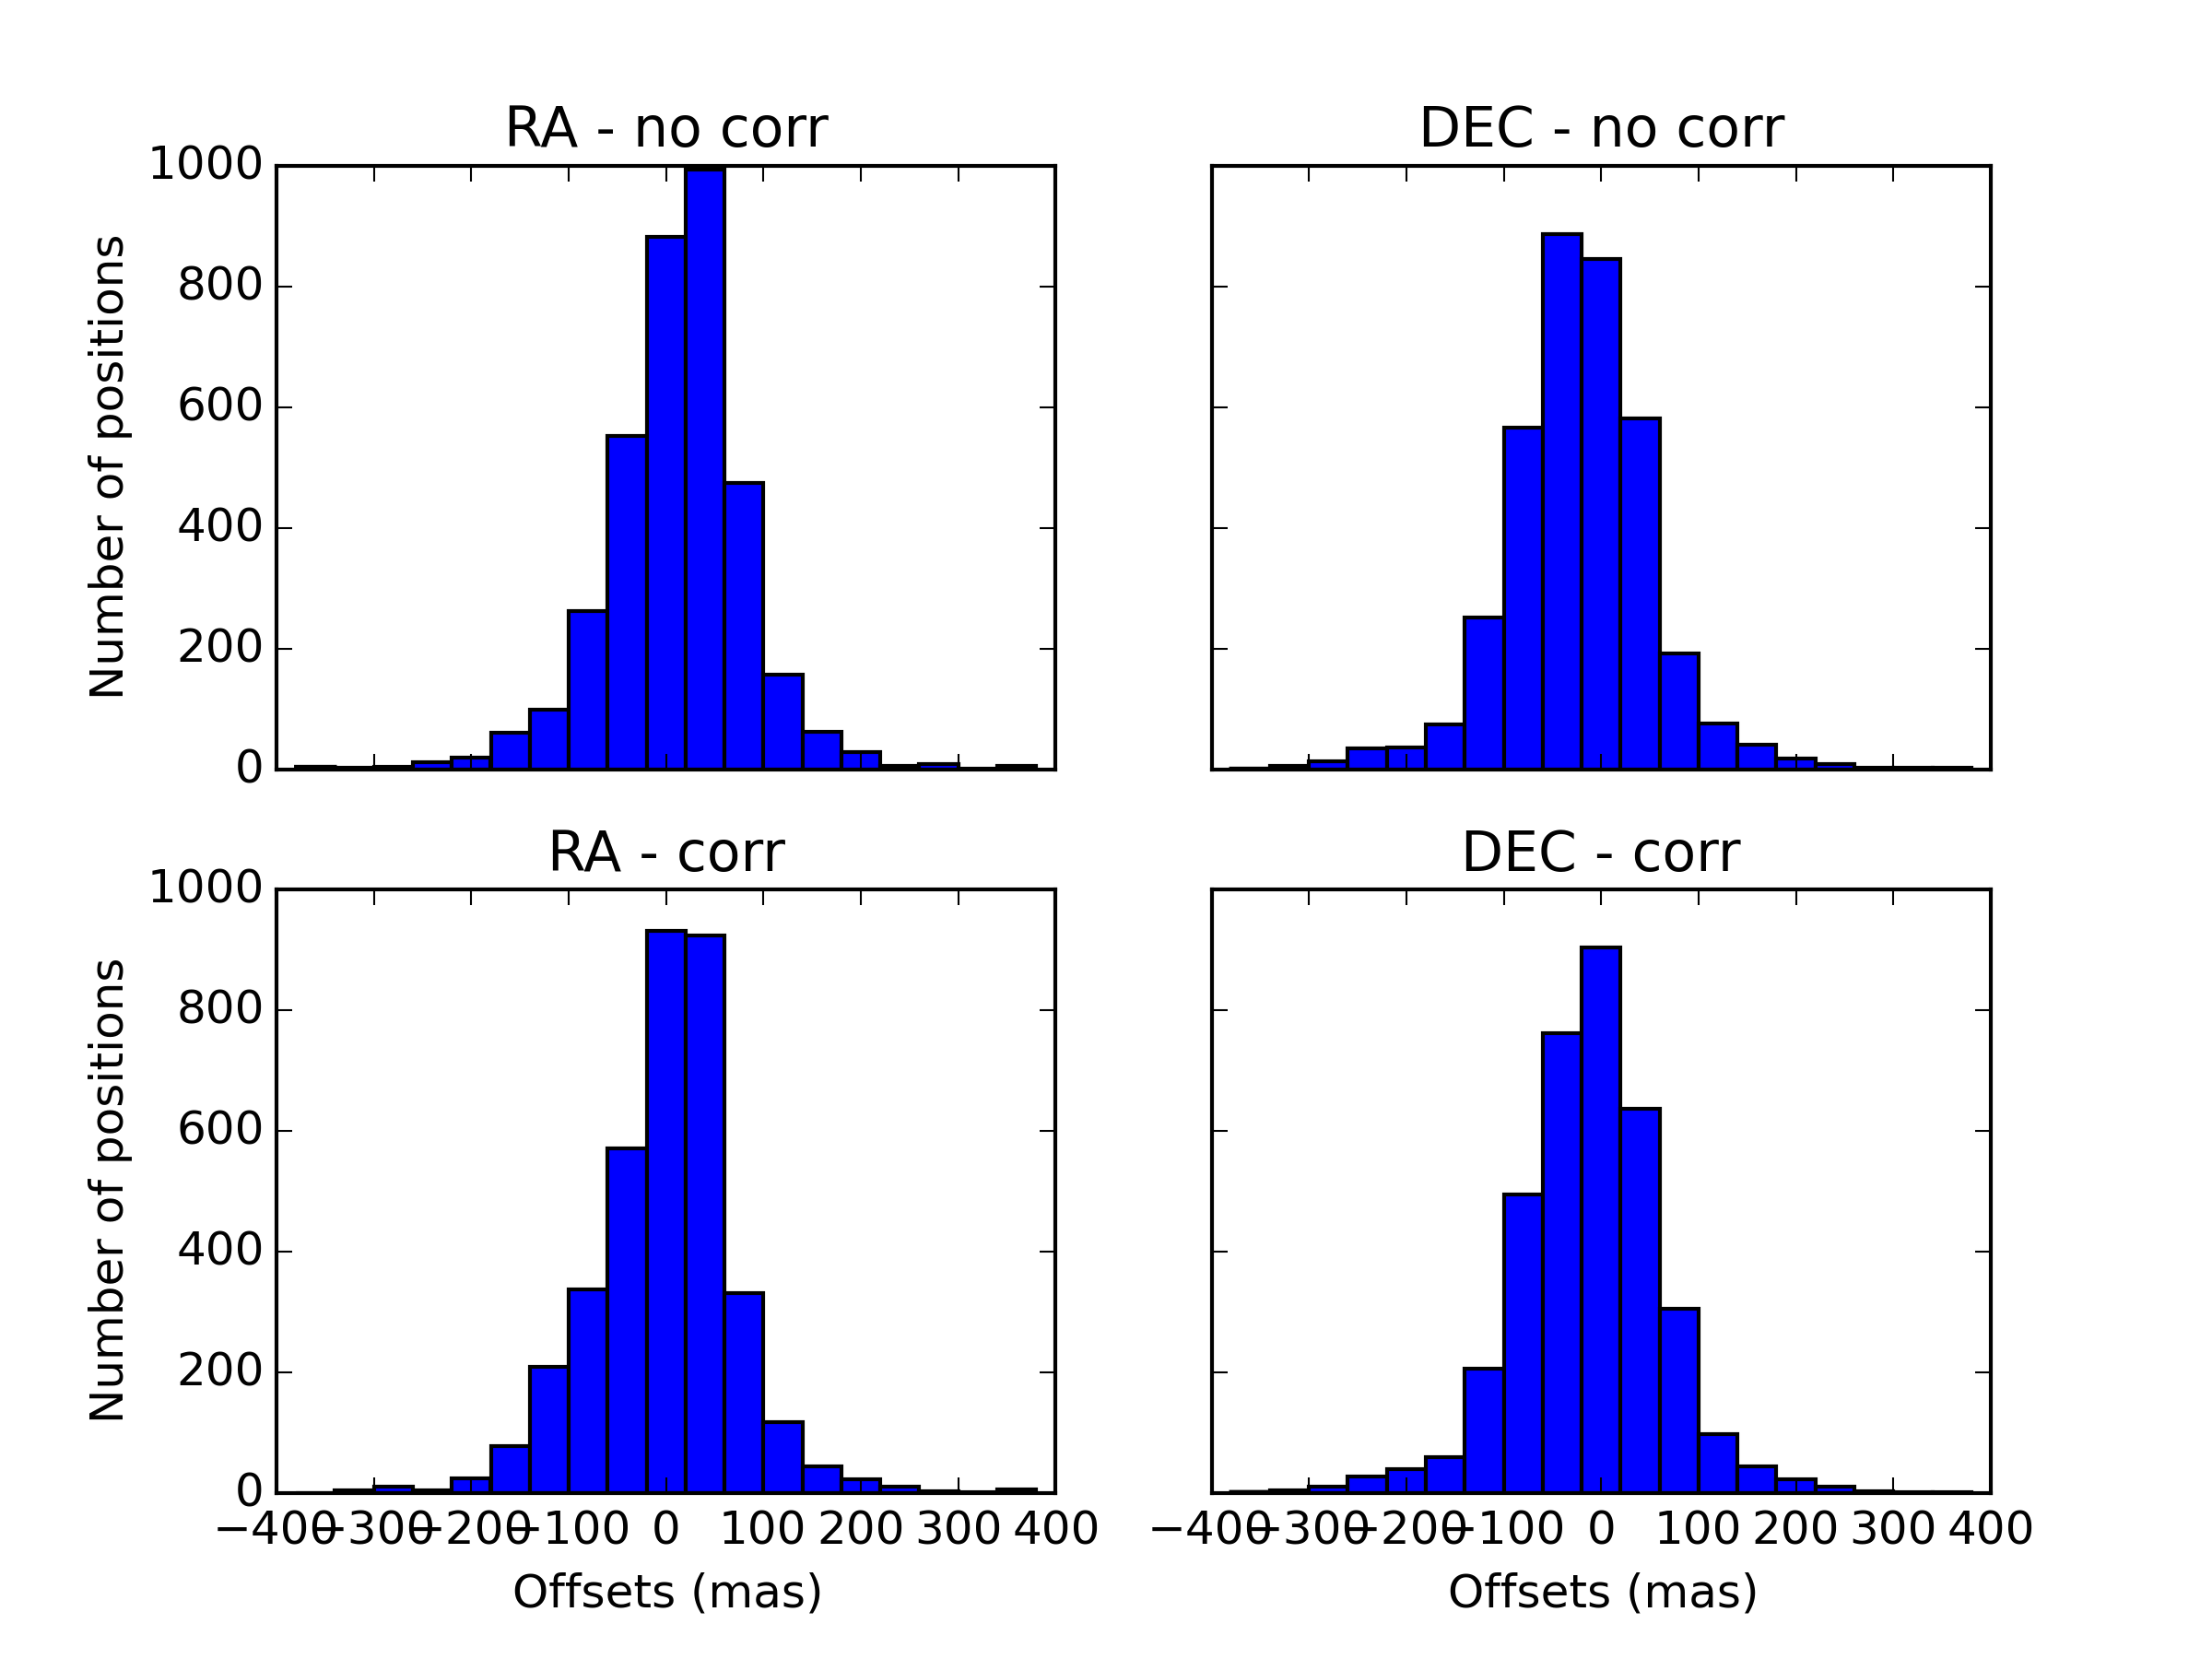
\includegraphics[width=17.0cm]{dist_Triton_IAG.png} 
\caption{Distribution of the offsets of Triton observed in IAG.}
\label{Fig:refraction-tri-iag}
\end{figure}

\begin{landscape}

Table \ref{Tab:parameters} show respective nights used in the Figs. \ref{Fig:refraction-net-160}-\ref{Fig:refraction-tri-iag}, the filter, the variation in hour angle ($\Delta H$), the parameters obtained ($\Delta B$), number of images (Nimg), mean number of reference stars (Nstars) and mean offsets before and after correction. It is possible to see that the $\Delta B$ calculated has high values for Neptune, while for Triton they are smaller.

For the nights with observations distributed in a smaller time interval, it must be used $\Delta B$ of close nights observed with the same filter for the correction.

\begin{longtable}{|l|c|c|c|c|c|c|c|c|c|c|}
\caption{Obtained parameters and offsets from adjustments. Only nights with $\Delta H > 1.5h$.\label{Tab:parameters}}\\
\hline
\multicolumn{10}{|c|}{Neptune-160}\\
Date & Filter & $\Delta H$ & $\Delta B$ & Nimg & Nstars & RA no corr & DEC no corr & RA corr & DEC corr \\
%\hline
\hline
\endfirsthead
\multicolumn{10}{c}%
{\tablename\ \thetable\ -- \textit{Continued from previous page}} \\
\hline
Date & Filter & $\Delta H$ & $\Delta B$ & Nimg & Nstars & RA no corr & DEC no corr & RA corr & DEC corr \\
\hline
\endhead
\hline \multicolumn{10}{r}{\textit{Continued on next page}} \\
\endfoot
\hline
\endlastfoot
%\begin{table*}
%\begin{tabular}{|l|c|c|c|c|c|c|c|c|c|c|}
%\hline
%Date & Filter & $\Delta H$ & $\Delta B$ & Nimg & Nstars & RA no corr & DEC no corr & RA corr & DEC corr \\
\hline
1992-06-09 & Clear & 1.57 & +0.29$\pm$0.03 &  13 &  11 &  190$\pm$ 54 &   25$\pm$ 76 &  -43$\pm$ 15 &   65$\pm$ 68 \\ 
1992-07-19 & Clear & 1.63 & +0.20$\pm$0.04 &  17 &  24 &   50$\pm$ 46 &  117$\pm$ 37 &    1$\pm$ 26 &  125$\pm$ 36 \\ 
1993-06-24 & Clear & 1.61 & -0.07$\pm$0.04 &  10 &  17 &  -17$\pm$ 26 &  -38$\pm$ 48 &  -21$\pm$ 22 &  -40$\pm$ 48 \\ 
1993-06-25 & Clear & 2.63 & +0.03$\pm$0.02 &  12 &   8 &  -37$\pm$ 26 &   70$\pm$ 75 &  -40$\pm$ 24 &   72$\pm$ 74 \\ 
1993-08-20 & Clear & 3.35 & +0.20$\pm$0.02 &  31 &  29 &   15$\pm$ 76 &  -83$\pm$ 43 &   -7$\pm$ 34 &  -75$\pm$ 44 \\ 
1993-08-22 & Clear & 2.87 & +0.18$\pm$0.02 &  35 &   9 &  -47$\pm$ 63 &  -74$\pm$ 44 &  -15$\pm$ 38 &  -67$\pm$ 46 \\ 
1996-06-22 & Clear & 1.68 & +0.24$\pm$0.02 &  19 &  16 &  -25$\pm$ 51 &  -32$\pm$ 35 &  -48$\pm$ 18 &  -20$\pm$ 35 \\ 
1996-10-02 & Clear & 1.97 & +0.31$\pm$0.07 &  16 &   6 &  252$\pm$192 &  -60$\pm$ 73 &  -59$\pm$126 &   10$\pm$ 79 \\ 
1997-06-01 & Clear & 4.89 & +0.35$\pm$0.03 &  91 &  11 & -155$\pm$189 & -112$\pm$ 36 & -120$\pm$107 &  -81$\pm$ 40 \\ 
1997-06-02 & Clear & 5.24 & +0.22$\pm$0.01 &  60 &  10 & -113$\pm$125 &  -84$\pm$ 36 &  -73$\pm$ 48 &  -61$\pm$ 33 \\ 
1998-06-06 & Clear & 2.51 & +0.38$\pm$0.04 &  35 &  11 & -140$\pm$101 &  -66$\pm$ 42 &  -13$\pm$ 56 &  -33$\pm$ 41 \\ 
1998-09-03 & Clear & 1.52 & +0.30$\pm$0.03 &  20 &  10 &  -86$\pm$ 63 &  -75$\pm$ 49 &   20$\pm$ 26 &  -51$\pm$ 47 \\ 
\hline
\multicolumn{10}{|c|}{Triton-160}\\
Date & Filter & $\Delta H$ & $\Delta B$ & Nimg & Nstars & RA no corr & DEC no corr & RA corr & DEC corr \\
\hline
1992-06-09 & Clear & 1.57 & +0.01$\pm$0.03 &  16 &  16 &   12$\pm$ 20 &   19$\pm$ 79 &    3$\pm$ 20 &   20$\pm$ 79 \\ 
1992-07-19 & Clear & 1.89 & +0.07$\pm$0.04 &  21 &  25 &   -3$\pm$ 33 &   15$\pm$ 52 &  -21$\pm$ 30 &   17$\pm$ 52 \\ 
1993-06-24 & Clear & 1.61 & +0.01$\pm$0.04 &  15 &  13 &    8$\pm$ 23 &   15$\pm$ 55 &    9$\pm$ 23 &   16$\pm$ 55 \\ 
1993-06-25 & Clear & 2.90 & -0.09$\pm$0.04 &  20 &  12 &  -28$\pm$ 60 &   36$\pm$ 79 &  -14$\pm$ 52 &   32$\pm$ 80 \\ 
1993-08-20 & Clear & 3.35 & -0.01$\pm$0.02 &  30 &  27 &   -8$\pm$ 29 &  -25$\pm$ 62 &   -6$\pm$ 29 &  -25$\pm$ 62 \\ 
1993-08-22 & Clear & 3.12 & +0.05$\pm$0.01 &  43 &  13 &   -2$\pm$ 28 &   -9$\pm$ 43 &    4$\pm$ 24 &   -7$\pm$ 43 \\ 
1994-09-22 & Clear & 1.94 & -0.12$\pm$0.08 &  13 &  12 &  -33$\pm$ 53 &   30$\pm$ 75 &   48$\pm$ 49 &   16$\pm$ 71 \\ 
1994-09-22 & Clear & 1.55 & +0.00$\pm$0.04 &  15 &  17 &  -53$\pm$ 21 &   24$\pm$ 82 &  -54$\pm$ 21 &   24$\pm$ 82 \\ 
1995-08-07 & Clear & 3.02 & +0.02$\pm$0.02 &  11 &  21 &  -10$\pm$ 14 &  -40$\pm$ 30 &  -10$\pm$ 13 &  -39$\pm$ 30 \\ 
1996-06-22 & Clear & 2.28 & -0.08$\pm$0.02 &  32 &  15 &  -87$\pm$ 24 &   -9$\pm$ 29 &  -77$\pm$ 19 &  -13$\pm$ 28 \\ 
1996-08-22 & Clear & 1.56 & +0.01$\pm$0.02 &  29 &  13 &   43$\pm$ 30 &  -41$\pm$ 44 &   37$\pm$ 30 &  -40$\pm$ 44 \\ 
1996-08-24 & Clear & 1.99 & -0.03$\pm$0.04 &  10 &  11 &   46$\pm$ 15 &  -66$\pm$ 23 &   52$\pm$ 15 &  -67$\pm$ 23 \\ 
1996-10-02 & Clear & 1.97 & +0.04$\pm$0.07 &  16 &   6 &   73$\pm$121 &    1$\pm$ 76 &   38$\pm$120 &    9$\pm$ 77 \\ 
1997-06-01 & Clear & 4.89 & +0.11$\pm$0.01 & 101 &  11 &  -76$\pm$ 71 & -107$\pm$ 53 &  -68$\pm$ 51 &  -98$\pm$ 54 \\ 
1997-06-02 & Clear & 5.41 & +0.02$\pm$0.02 &  81 &  10 &  -18$\pm$ 86 &  -56$\pm$ 30 &  -17$\pm$ 85 &  -54$\pm$ 30 \\ 
1997-08-11 & Clear & 3.08 & +0.12$\pm$0.02 &  33 &  11 &  -30$\pm$ 46 &  -23$\pm$ 27 &    2$\pm$ 28 &  -14$\pm$ 28 \\ 
1997-08-13 & Clear & 1.67 & +0.04$\pm$0.03 &  19 &   6 &   44$\pm$ 30 &   -4$\pm$ 16 &   60$\pm$ 29 &   -0$\pm$ 16 \\ 
1998-06-06 & Clear & 2.84 & +0.13$\pm$0.04 &  42 &  11 &  -46$\pm$ 62 &  -55$\pm$ 33 &   -5$\pm$ 53 &  -44$\pm$ 33 \\ 
1998-09-03 & Clear & 1.52 & -0.04$\pm$0.04 &  20 &  10 &    3$\pm$ 36 &  -48$\pm$ 54 &  -11$\pm$ 35 &  -50$\pm$ 54 \\ 
1999-06-06 & Clear & 1.58 & +0.23$\pm$0.04 &  27 &  14 &   19$\pm$ 47 &  -63$\pm$ 43 &   91$\pm$ 32 &  -43$\pm$ 40 \\ 
1999-08-22 & Clear & 3.06 & +0.03$\pm$0.02 &  30 &  15 &  -32$\pm$ 37 &   -7$\pm$ 25 &  -45$\pm$ 35 &   -3$\pm$ 26 \\ 
\hline
\multicolumn{10}{|c|}{Neptune-IAG}\\
Date & Filter & $\Delta H$ & $\Delta B$ & Nimg & Nstars & RA no corr & DEC no corr & RA corr & DEC corr \\
\hline
2001-08-26 & B     & 2.11 & +0.15$\pm$0.03 &  44 &  15 &   89$\pm$ 55 &  -41$\pm$ 57 &   14$\pm$ 41 &  -22$\pm$ 57 \\ 
2002-07-15 & Clear & 6.11 & +0.18$\pm$0.00 &  57 &  17 &   51$\pm$163 &   85$\pm$ 90 &  -36$\pm$ 31 &  131$\pm$ 76 \\ 
2002-07-18 & Clear & 3.86 & +0.21$\pm$0.02 &  30 &  13 & -100$\pm$115 & -140$\pm$ 61 &  -50$\pm$ 61 & -111$\pm$ 61 \\ 
2003-07-22 & Clear & 2.38 & +0.33$\pm$0.04 &  20 &  15 &  174$\pm$137 &  -75$\pm$ 80 &  -32$\pm$ 57 &  -13$\pm$ 74 \\ 
2003-07-23 & Clear & 4.08 & +0.02$\pm$0.01 &  39 &  16 &  -81$\pm$ 36 &   13$\pm$ 55 &  -78$\pm$ 34 &   17$\pm$ 55 \\ 
2003-07-25 & Clear & 6.19 & -0.01$\pm$0.02 &  21 &   9 & -107$\pm$ 74 &    9$\pm$ 62 & -106$\pm$ 74 &    7$\pm$ 62 \\ 
2003-07-26 & Clear & 6.97 & -0.01$\pm$0.08 &  17 &  10 & -132$\pm$211 &    8$\pm$123 & -129$\pm$211 &    7$\pm$124 \\ 
2003-07-27 & Clear & 1.54 & +0.06$\pm$0.06 &  26 &  14 &  -21$\pm$104 &    4$\pm$ 84 &  -90$\pm$102 &   24$\pm$ 84 \\ 
2003-07-28 & Clear & 7.98 & +0.01$\pm$0.03 &  43 &  12 &  -37$\pm$144 &   21$\pm$162 &  -44$\pm$144 &   24$\pm$162 \\ 
2003-08-20 & Clear & 4.03 & +0.26$\pm$0.04 &  30 &  17 &   95$\pm$154 &  -72$\pm$ 66 &   18$\pm$ 98 &  -35$\pm$ 60 \\ 
2003-10-14 & V     & 2.33 & +0.02$\pm$0.03 &   8 &  30 &   20$\pm$ 25 &   16$\pm$ 31 &   16$\pm$ 25 &   18$\pm$ 31 \\ 
2004-08-05 & V     & 2.21 & -0.03$\pm$0.12 &   5 &   6 &  -53$\pm$ 67 &  -61$\pm$ 25 &  -35$\pm$ 67 &  -66$\pm$ 26 \\ 
2004-08-06 & V     & 3.10 & +0.18$\pm$0.03 &   4 &   6 & -160$\pm$ 61 & -173$\pm$ 60 & -165$\pm$ 14 & -151$\pm$ 59 \\ 
2004-08-07 & V     & 4.31 & +0.21$\pm$0.33 &   6 &  11 &  128$\pm$333 &  -40$\pm$210 &  110$\pm$317 &   -9$\pm$212 \\ 
2004-08-21 & Clear & 4.09 & +0.08$\pm$0.02 &  30 &  21 &  -32$\pm$ 57 &  -78$\pm$ 55 &  -56$\pm$ 44 &  -66$\pm$ 57 \\ 
2004-08-21 & Clear & 2.57 & +0.05$\pm$0.02 &  30 &  21 &  -42$\pm$ 28 &  -86$\pm$ 41 &  -32$\pm$ 26 &  -81$\pm$ 41 \\ 
2004-08-23 & Clear & 5.20 & +0.06$\pm$0.01 &  70 &  18 &   10$\pm$ 59 &  -88$\pm$ 52 &  -29$\pm$ 42 &  -73$\pm$ 50 \\ 
2004-08-24 & Clear & 3.94 & +0.06$\pm$0.01 &  40 &  18 &   -2$\pm$ 34 &  -83$\pm$ 66 &  -23$\pm$ 26 &  -74$\pm$ 65 \\ 
2004-09-24 & R     & 3.08 & +0.27$\pm$0.05 &  35 &  13 &  157$\pm$183 &   12$\pm$136 &   -0$\pm$133 &   63$\pm$126 \\ 
2004-09-25 & Clear & 3.75 & +0.26$\pm$0.03 &  40 &  14 &  201$\pm$164 &    2$\pm$ 93 &   37$\pm$106 &   54$\pm$ 86 \\ 
2005-09-24 & V     & 2.78 & +0.05$\pm$0.01 &  88 &  14 &    2$\pm$ 47 & -101$\pm$ 61 &  -52$\pm$ 44 &  -85$\pm$ 60 \\ 
2006-06-08 & Clear & 2.68 & +0.32$\pm$0.04 &  95 &  24 &  -91$\pm$144 &  -83$\pm$ 93 &   14$\pm$115 &  -30$\pm$ 93 \\ 
2011-09-26 & I     & 4.02 & +0.05$\pm$0.00 & 250 &  18 &   76$\pm$ 44 &  -67$\pm$ 48 &   38$\pm$ 36 &  -52$\pm$ 45 \\ 
2012-10-19 & R     & 1.99 & +0.13$\pm$0.03 & 119 &   8 &   41$\pm$100 & -167$\pm$137 &  -50$\pm$ 92 & -130$\pm$138 \\ 
\hline
\multicolumn{10}{|c|}{Triton-IAG}\\
Date & Filter & $\Delta H$ & $\Delta B$ & Nimg & Nstars & RA no corr & DEC no corr & RA corr & DEC corr \\
\hline
2001-08-26 & B     & 2.11 & +0.03$\pm$0.03 &  24 &  15 &    1$\pm$ 40 &  -53$\pm$ 46 &  -13$\pm$ 39 &  -50$\pm$ 46 \\ 
2002-07-15 & Clear & 6.11 & +0.01$\pm$0.00 &  55 &  17 &   14$\pm$ 27 &  -29$\pm$ 45 &    7$\pm$ 24 &  -26$\pm$ 45 \\ 
2002-07-18 & Clear & 3.86 & -0.01$\pm$0.03 &  31 &  13 &   25$\pm$ 74 &  -68$\pm$111 &   23$\pm$ 74 &  -69$\pm$111 \\ 
2003-07-22 & Clear & 2.55 & +0.08$\pm$0.02 &  31 &  17 &   -8$\pm$ 57 &   -7$\pm$ 53 &  -58$\pm$ 49 &    8$\pm$ 54 \\ 
2003-07-23 & Clear & 4.08 & +0.04$\pm$0.02 &  38 &  16 &  -44$\pm$ 54 &  -12$\pm$ 45 &  -37$\pm$ 50 &   -6$\pm$ 45 \\ 
2003-07-25 & Clear & 6.39 & -0.04$\pm$0.03 &  44 &  16 &  -60$\pm$138 &    9$\pm$ 50 &  -64$\pm$136 &    2$\pm$ 51 \\ 
2003-07-26 & Clear & 6.97 & -0.04$\pm$0.04 &  33 &  14 & -133$\pm$167 &   21$\pm$ 90 & -121$\pm$165 &   13$\pm$ 91 \\ 
2003-07-27 & Clear & 1.54 & +0.01$\pm$0.05 &  26 &  14 &  -31$\pm$ 76 &   31$\pm$ 74 &  -40$\pm$ 76 &   34$\pm$ 74 \\ 
2003-07-28 & Clear & 7.98 & -0.01$\pm$0.02 &  60 &  14 &  -51$\pm$130 &   46$\pm$133 &  -44$\pm$130 &   43$\pm$133 \\ 
2003-08-20 & Clear & 4.20 & +0.02$\pm$0.02 &  49 &  21 &   53$\pm$ 69 &   -8$\pm$ 45 &   46$\pm$ 68 &   -5$\pm$ 45 \\ 
2003-10-14 & V     & 3.63 & -0.04$\pm$0.03 &  20 &  33 &   -4$\pm$ 54 &  -34$\pm$ 72 &   13$\pm$ 53 &  -40$\pm$ 74 \\ 
2003-10-15 & V     & 2.27 & +0.01$\pm$0.05 &  18 &  33 &  -22$\pm$ 38 &   -3$\pm$ 78 &  -23$\pm$ 38 &   -2$\pm$ 77 \\ 
2003-10-16 & V     & 1.94 & -0.10$\pm$0.10 &   8 &  25 &  -18$\pm$ 64 &  -15$\pm$ 36 &   46$\pm$ 58 &  -32$\pm$ 32 \\ 
2003-10-17 & V     & 2.09 & +0.02$\pm$0.04 &  10 &  29 &    1$\pm$ 31 &    4$\pm$ 92 &   -7$\pm$ 31 &    7$\pm$ 92 \\ 
2003-10-19 & V     & 1.89 & -0.12$\pm$0.05 &  12 &  31 &   -7$\pm$ 40 &  -45$\pm$ 35 &   44$\pm$ 32 &  -60$\pm$ 32 \\ 
2004-08-05 & V     & 2.38 & -0.06$\pm$0.02 &  21 &  15 &  -13$\pm$ 31 & -101$\pm$ 35 &   21$\pm$ 26 & -111$\pm$ 35 \\ 
2004-08-06 & V     & 3.27 & +0.06$\pm$0.07 &  22 &  16 &   53$\pm$ 99 & -110$\pm$ 50 &   45$\pm$ 97 & -102$\pm$ 50 \\ 
2004-08-07 & V     & 4.50 & +0.00$\pm$0.03 &  23 &  19 &   54$\pm$ 56 & -117$\pm$ 61 &   54$\pm$ 56 & -117$\pm$ 61 \\ 
2004-08-20 & Clear & 3.81 & +0.03$\pm$0.01 &  16 &  24 &   -5$\pm$ 26 &  -40$\pm$ 24 &  -15$\pm$ 23 &  -35$\pm$ 23 \\ 
2004-08-21 & Clear & 4.09 & +0.02$\pm$0.02 &  27 &  22 &  -13$\pm$ 41 &  -32$\pm$ 52 &  -22$\pm$ 39 &  -28$\pm$ 53 \\ 
2004-08-21 & Clear & 2.57 & +0.01$\pm$0.02 &  26 &  21 &  -13$\pm$ 28 &  -51$\pm$ 35 &  -12$\pm$ 27 &  -51$\pm$ 35 \\ 
2004-08-23 & Clear & 5.20 & +0.02$\pm$0.01 &  43 &  18 &   -2$\pm$ 44 &  -36$\pm$ 49 &  -11$\pm$ 42 &  -32$\pm$ 49 \\ 
2004-08-24 & Clear & 3.94 & +0.02$\pm$0.01 &  29 &  17 &   -2$\pm$ 29 &  -34$\pm$ 62 &   -9$\pm$ 28 &  -31$\pm$ 62 \\ 
2004-09-24 & R     & 3.08 & +0.04$\pm$0.04 &  37 &  14 &   26$\pm$111 &   83$\pm$131 &    2$\pm$109 &   91$\pm$130 \\ 
2004-09-25 & Clear & 3.75 & +0.01$\pm$0.04 &  36 &  14 &   59$\pm$113 &   91$\pm$ 77 &   51$\pm$113 &   93$\pm$ 77 \\ 
2005-09-24 & V     & 2.78 & +0.01$\pm$0.01 & 155 &  16 &  -14$\pm$ 43 &  -95$\pm$ 56 &  -26$\pm$ 43 &  -91$\pm$ 56 \\ 
2006-06-08 & Clear & 3.30 & +0.10$\pm$0.03 & 157 &  26 &  -22$\pm$104 &  -47$\pm$ 69 &    2$\pm$100 &  -32$\pm$ 69 \\ 
2009-07-22 & Clear & 2.19 & +0.08$\pm$0.07 &  17 &  15 &   10$\pm$ 43 &   74$\pm$ 96 &   -1$\pm$ 41 &   87$\pm$ 95 \\ 
2011-09-05 & I     & 1.82 & +0.19$\pm$0.03 & 100 &  18 &   91$\pm$ 47 &   -1$\pm$ 34 &   36$\pm$ 38 &   38$\pm$ 36 \\ 
2011-09-26 & I     & 4.02 & -0.00$\pm$0.00 & 250 &  18 &   43$\pm$ 28 &    4$\pm$ 41 &   43$\pm$ 28 &    3$\pm$ 41 \\ 
2012-10-19 & R     & 1.99 & +0.13$\pm$0.03 & 118 &   8 &   14$\pm$108 &  -76$\pm$134 &  -78$\pm$100 &  -38$\pm$136 \\ 
\hline
\end{longtable}

%\end{tabular}
%\label{Tab:netuno-160}
%\caption{Obtained parameters and offsets from adjustments of 160 images for Neptune.}
%\end{table*}

\end{landscape}


%Teoretically, the difference in the positions of the objects in the sense Triton - Neptune compared to the difference in the ephemeris over a night would cause the following effects.
%
%\begin{itemize}
%\item RA: the difference in the offsets would be positives in the East side of the sky, negative in the West side and zero in the culmination, with the assumption that only chromatic refraction affects the offsets.
%\item DEC: the difference in the offsets in the culmination would be positive (Neptune is in the North side in both nights for the site). Farther from the culmination the difference in the offsets would be more positive.
%\end{itemize}
%
%Fig \ref{Fig:refraction} clearly shows that that the chromatic refraction is affecting the offsets confirming our expectation. It is possible to see that the distribution of the offsets for the 5 night are very similar over the hour angles observed.
%
%The offsets corrected by chromatic refraction of the 5 nights is presented in Fig. \ref{Fig:refraction-cor}.
%
%\begin{figure}[h]
%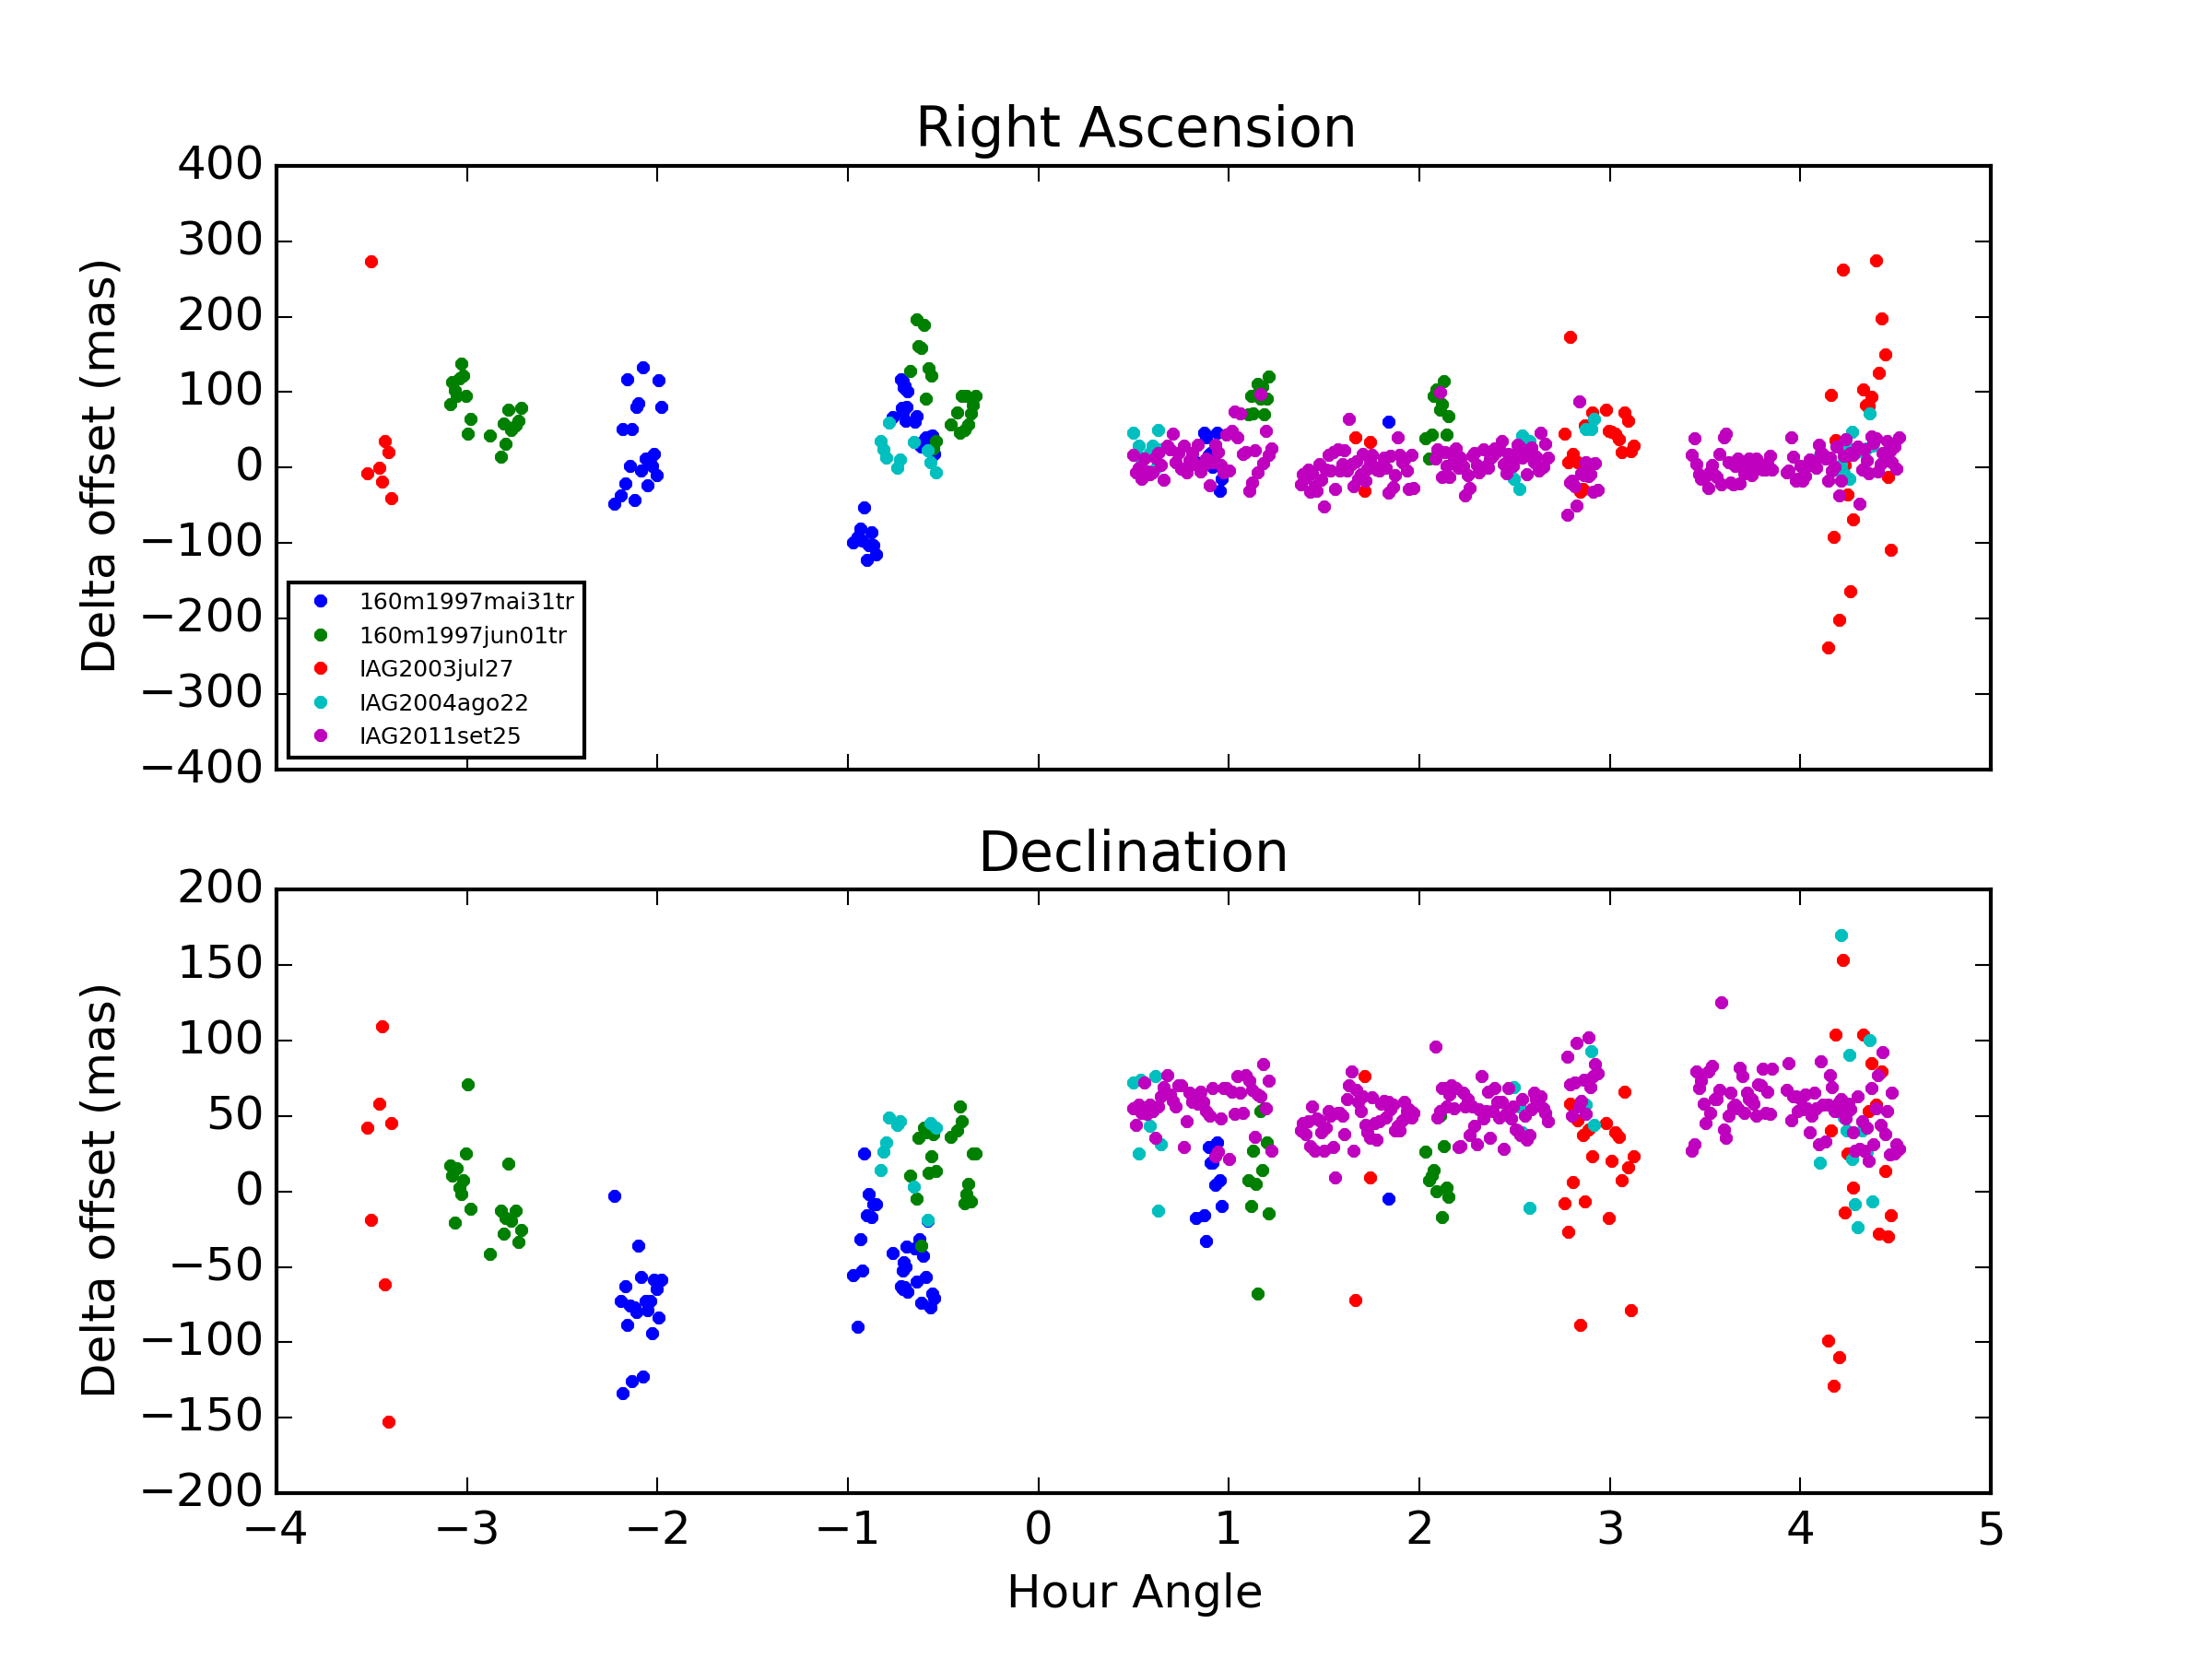
\includegraphics[width=16.0cm]{plot_hour_dif_cor.png} 
%\caption{Same as in Fig. \ref{Fig:refraction} but corrected by chromatic refraction.}
%\label{Fig:refraction-cor}
%\end{figure}
%
%In Table \ref{Tab:refraction} it is shown the mean of the difference in the offsets of Triton and Neptune for each night and their dispersions. We made two tests in the chromatic refraction, the first one we made the correction in the difference of the offsets of both objects. In the second test we made the corrections in the offsets separately for each object, then we took the difference between them.
%
%\begin{table}[h]
%\centering
%\caption{Mean and Standard deviation of the difference in the offsets of Triton - Neptune before and after the chromatic refraction correction}
%\label{Tab:refraction}
%\begin{tabular}{|l|c|c|c|c|c|c|}
%\hline
% \multicolumn{1}{|c|}{Night} & \multicolumn{2}{|c|}{No correction} & \multicolumn{2}{|c|}{Correction 1} & \multicolumn{2}{|c|}{Correction 2}\\
%  & RA & DEC & RA & DEC & RA & DEC \\
% \hline
%PE:1997-05-31 &   83+-138 & -1+-34 &  58+-88 & -22+-34 & 58+- 88 & -22+-34 \\
%PE:1997-06-01 &   120+-118 &  31+-26 &  84+-38 &  9+-27 & 84+-38 &  9+-27 \\
%BC:2003-07-27  &  -13+-111 & 25+-70 &  32+-70 &  7+-70 & 35+-100 &  6+-70 \\
%BC:2004-08-22  &   -11+-43 & 53+-38 &  22+-22 & 41+-37 & 19+- 23 & 42+-37 \\
%BC:2011-09-25  &   -33+-34 & 70+-17 &   5+-23 & 55+-16  &  5+- 23 & 55+-16 \\
%\hline
%\end{tabular}
%"Correction 1" means that the correction was made in the difference of the offsets of Triton and Neptune. "Correction 2" means that the correction of chromatic refraction was made in the offsets of Triton and Neptune separately then we took the difference between them.
%\end{table}
%
%It is possible to see that the dispersion of the offsets in RA after the correction is much smaller than before the correction. The mean offsets in RA also show significant difference. For DEC the dispersion does not change, but the mean offsets presents significant difference. It is also possible to see that the results for both tests are basically the same, with the exception of the night of 2003 in RA.
%
%In Table \ref{Tab:refraction-cor} it is shown the values of $\Delta B$ obtained in the fit of the offsets of Triton and Neptune separately and their differences. The minimum and maximum values of Hour Angle for each night is also presented.
%
%\begin{table}[h]
%\centering
%\caption{Results of the fit of $\Delta B$ in the 5 nights for the difference Triton - Neptune and for each object separately.}
%\label{Tab:refraction-cor}
%\begin{tabular}{|c|c|c|c|c|c|c|c|}
%\hline
% Night & Filter  & $H_{min}$ & $H_{max}$ & $\Delta H$ & Object & $\Delta B$ & err $\Delta B$\\
% \hline
% & &  & & & T-N  &     0.214  &  0.004   \\
% PE:1997-05-31 &   Clear & -3.0 & 2.1 & 5.1 & Neptune &   -0.219 &  0.004  \\
% & & & & & Triton &  -0.006  &  0.004 \\
%\hline
% & & & & & T-N  &  0.239  &  0.004 \\
% PE:1997-06-01 & Clear & -2.6 & 2.2 & 4.8 & Neptune &   -0.347  &  0.004 \\
% & & & & & Triton &   -0.107  &   0.004  \\
%\hline
% & & & & & T-N &   0.052 &   0.003  \\
%BC:2003-07-27 & Clear & -3.5 & 4.8 & 8.3 & Neptune &   -0.015  &  0.002  \\
% & & & & & Triton &    0.038  &  0.003  \\
%\hline
% & & & & & T-N &   0.048  &  0.004  \\
%BC:2004-08-22 & Clear? & -0.8 & 4.3 & 5.1 & Neptune &   -0.059  &   0.003  \\
% & & & & & Triton &   -0.015  &  0.004 \\
%\hline
%& & & & & T-N &   0.046  &  0.002  \\
%BC:2011-09-25 & I & 0.4 & 4.5 & 4.1 & Neptune &   -0.046  &   0.002  \\
% & & & & & Triton &    0.000  &  0.002   \\
%\hline
%\end{tabular}
%\end{table}

\section*{PSF for extended object test}

\section*{Final Remarks}

Fig \ref{Fig:netuno-all} shows the offsets of Neptune, respectively, in RA e DEC for all the positions not eliminated in the sigma-clip procedure. Fig \ref{Fig:netuno-media} shows the mean offsets of each night and respective discrepancy (error bars).

Fig \ref{Fig:triton-netuno-all} shows the difference between the relative observed positions and the relative ephemeris positions of Triton and Neptune in the sense Triton - Neptune where they were identified in the same frame and not eliminated by the sigma-clip procedure.

Fig \ref{Fig:triton-netuno-mean} shows the difference in the mean offsets night by night for all matched nights and not eliminated by the sigma-clip procedure in the sense Triton - Neptune. The dispersions (error bars) is the mean value of the dispersion in the night for each satellite.

%The large offsets found in 2002-2003 must be checked. It may be caused by few reference stars in the field or saturation.\\


It seems that there are long term systematic errors in the orbit of Neptune, and in the orbit of Triton around Neptune, but it is too soon to state that with confidence. We must still further refine the positions. We plan to do the following:

\begin{itemize}
\item Separate images by filter.
\item It may be required the use of a specific PSF for Neptune due to its large size.
\item Further refinements in the data may be needed as we further investigate these position sets.
\end{itemize}

%In Tables 2 and 3 it is shown the mean offsets in Right Ascension and Declination night by night for Neptune and Triton, respectively, observed in the \PE telescope. The dispersion of the positions (standard deviation), number of frames that was not eliminated by the sigma-clip procedure, the mean date of the night and the average number of reference stars by frame is also available in the tables. The respective mean offsets night by night for the \BC telescope is available in Tables 4 and 5. As for the previous telescopes, tables 6 and 7 summarizes the offsets obtained with the Zeiss telescope.

 %The average dispersion of the offsets in Tables 2-7 is also presented in the table.


\begin{figure}[h]
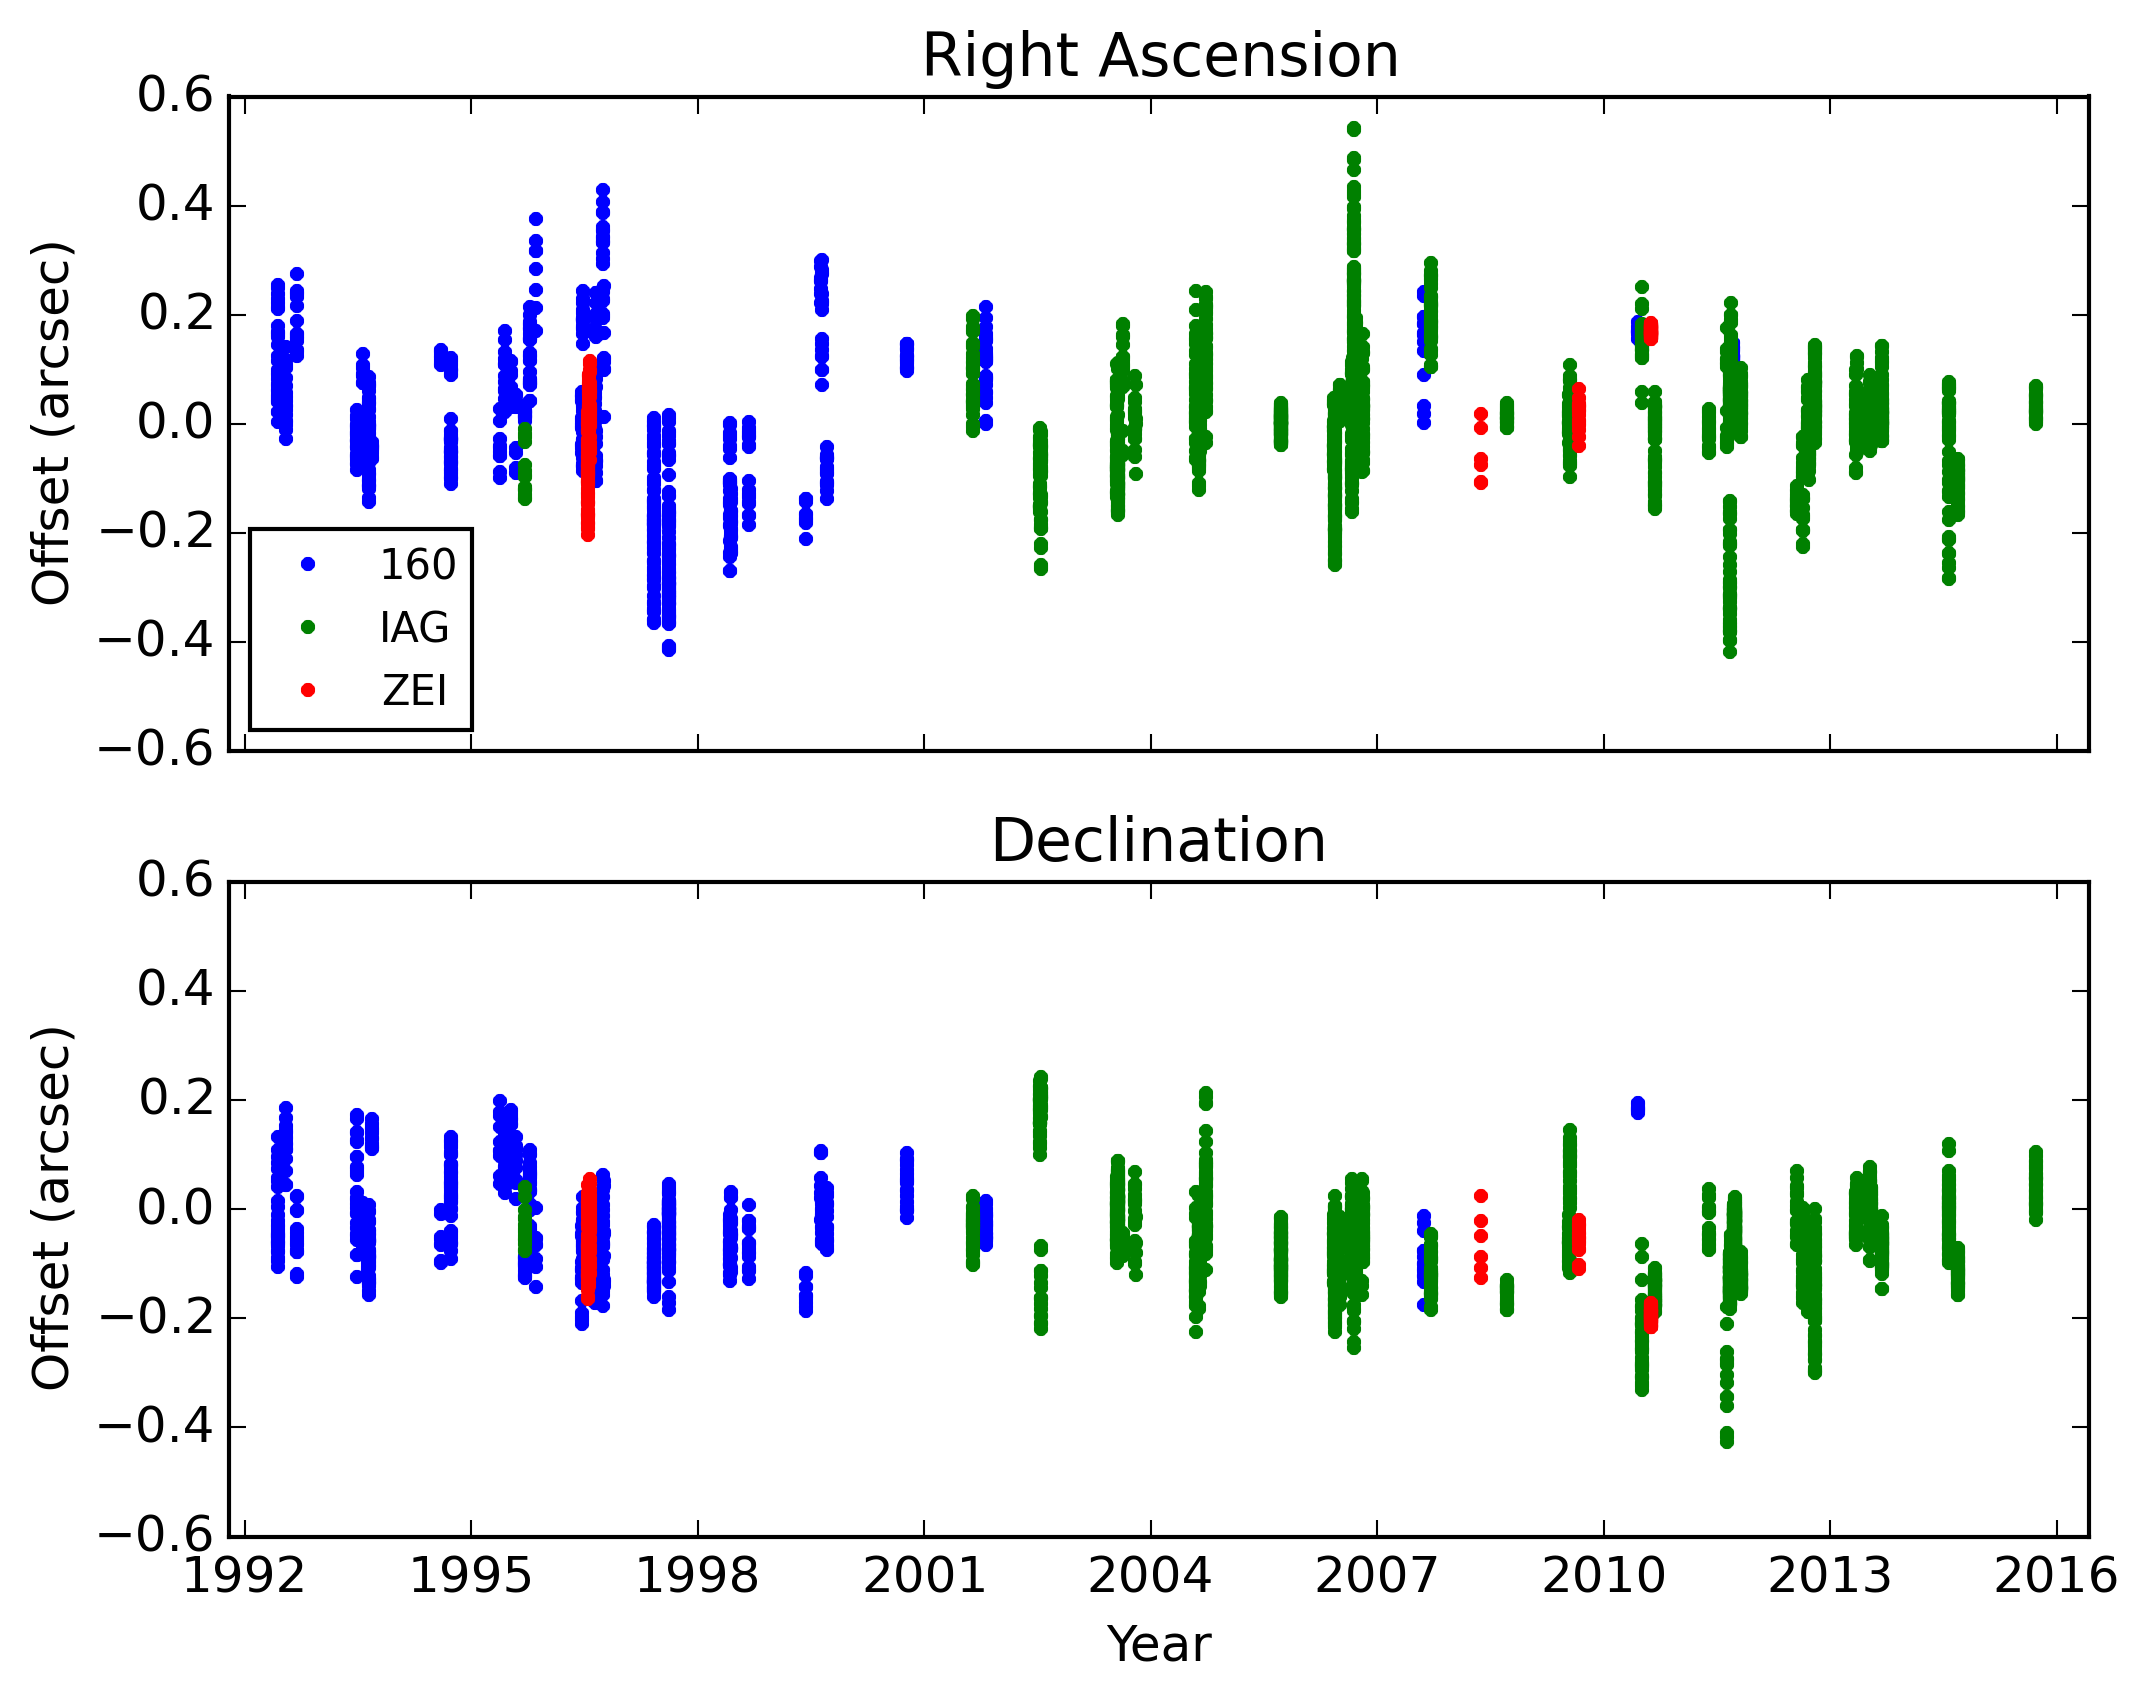
\includegraphics[width=16.0cm]{Netuno_all.png} 
\caption{Neptune - All Offsets}
\label{Fig:netuno-all}
\end{figure}
\begin{figure}
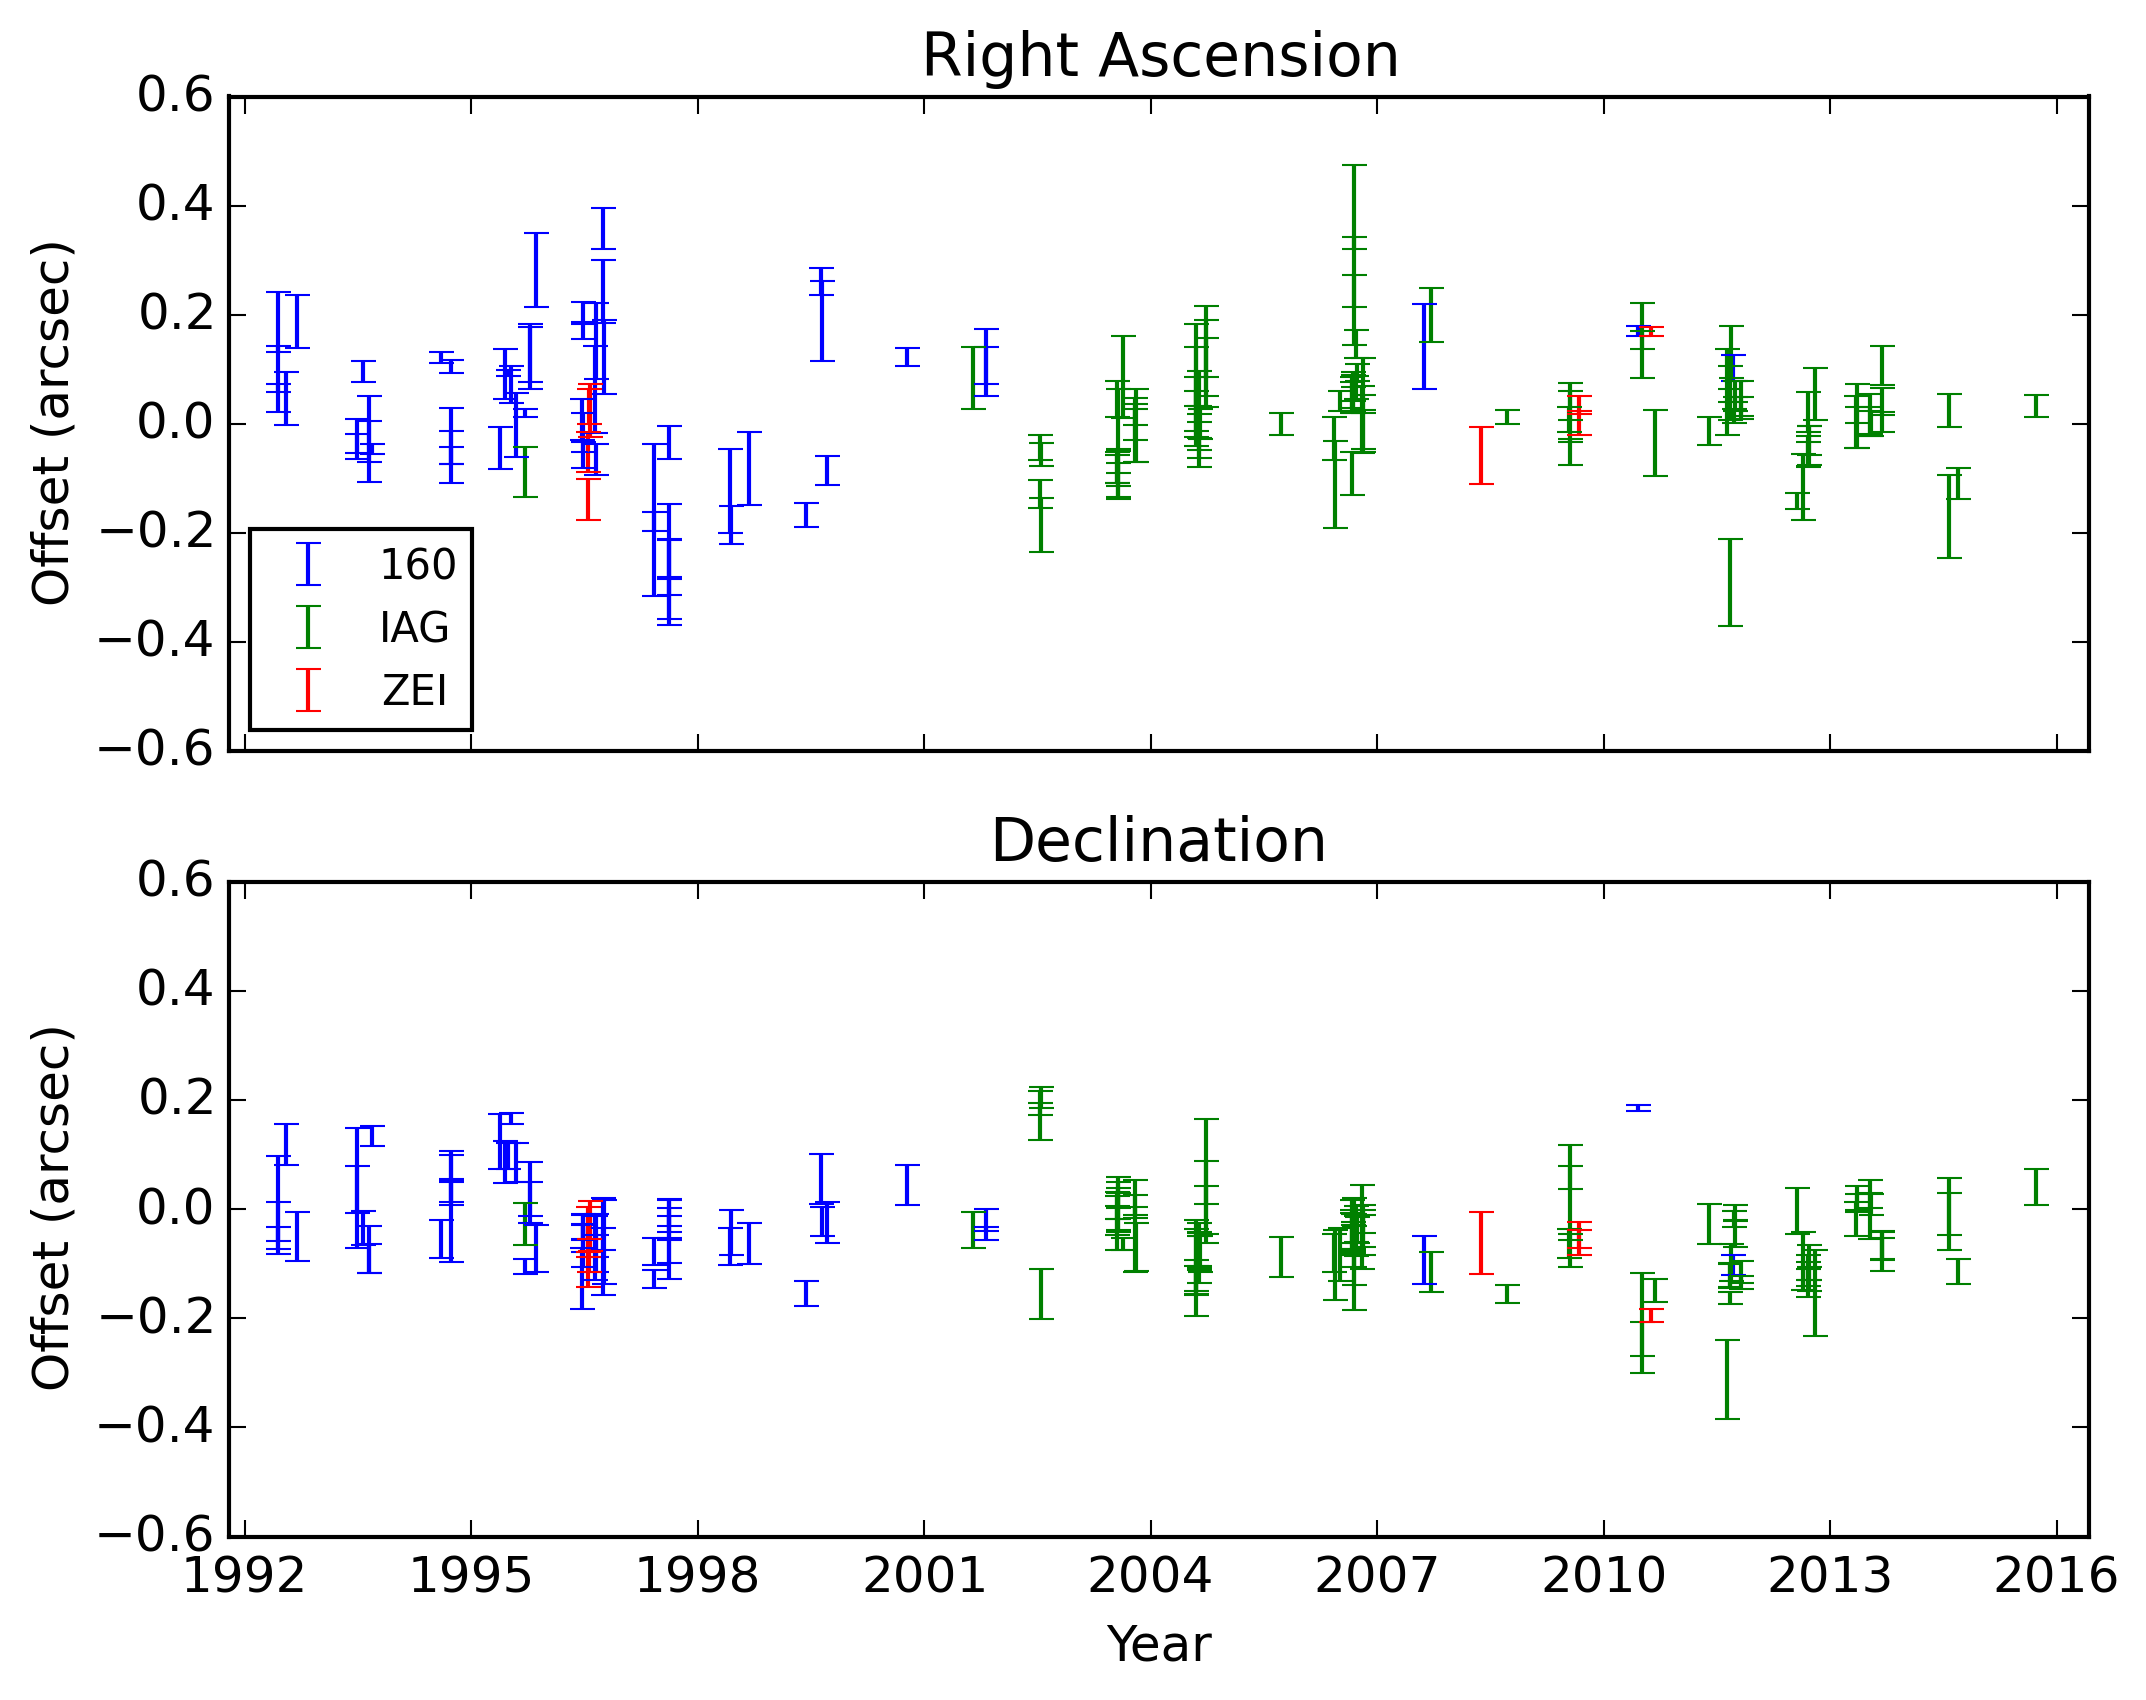
\includegraphics[width=16.0cm]{Netuno_media.png} 
\caption{Neptune - Mean offsets by day}
\label{Fig:netuno-media}
\end{figure}
%\begin{figure}
%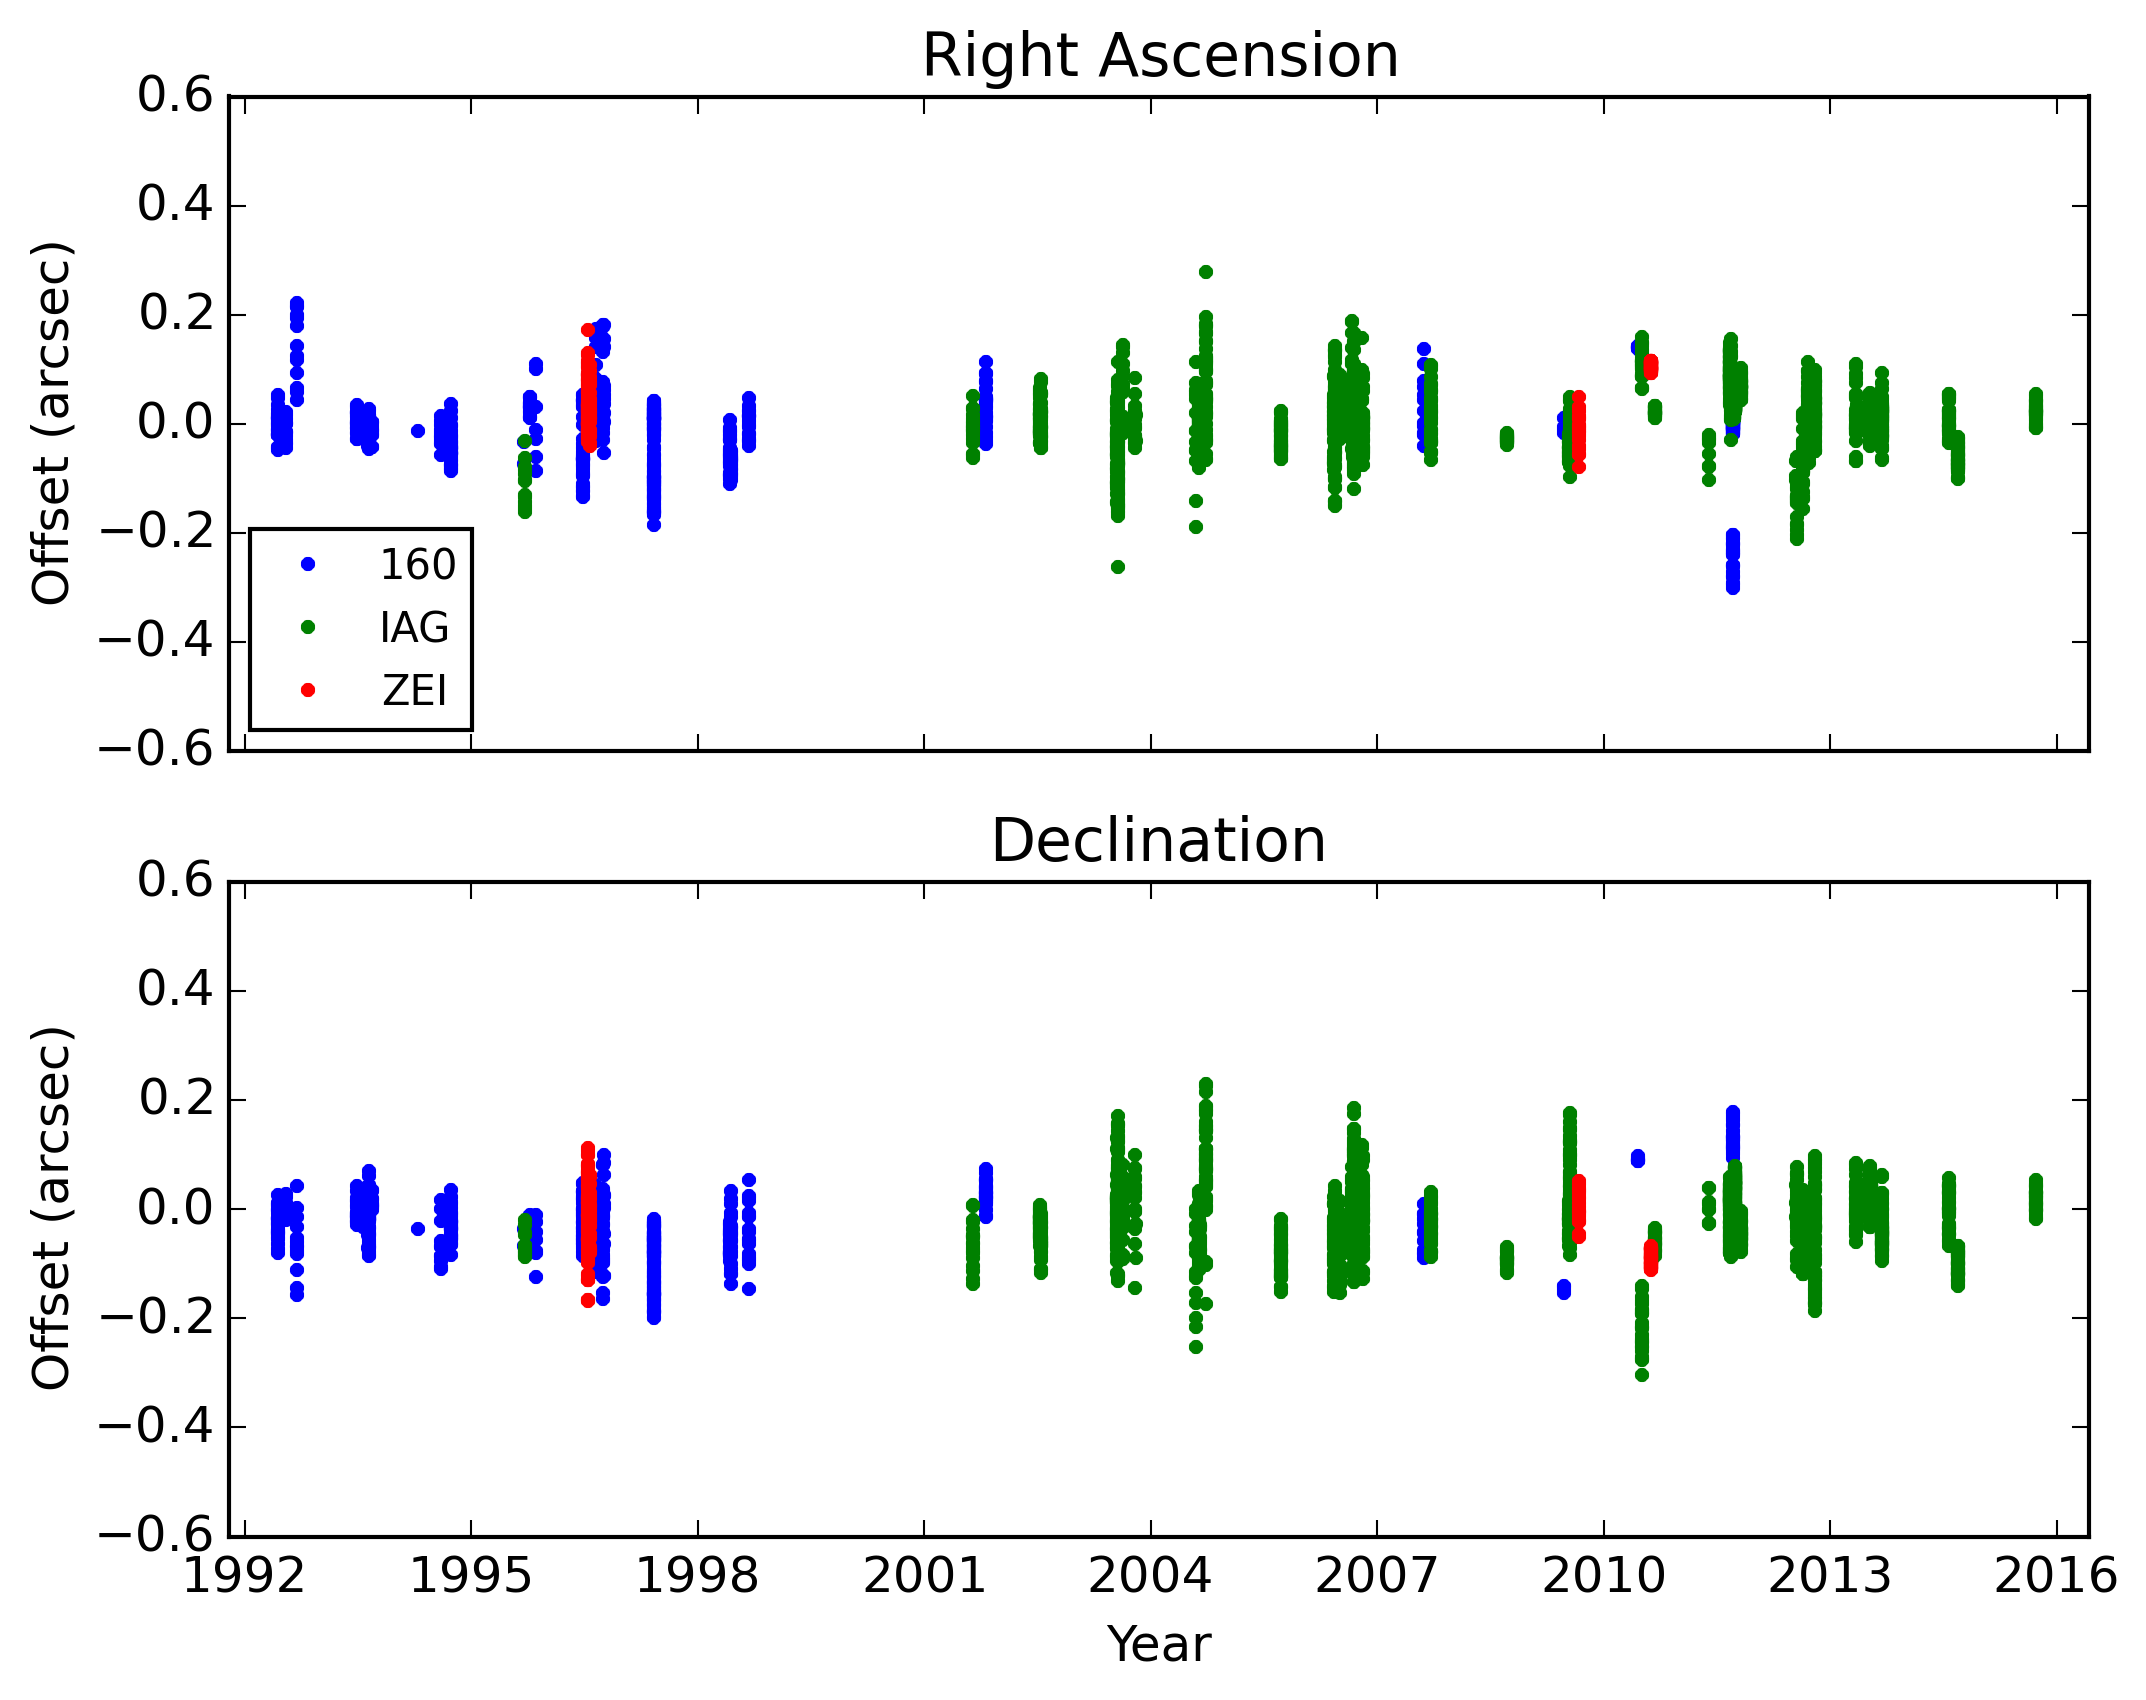
\includegraphics[width=16.0cm]{Triton_all.png} 
%\caption{Triton - All Offsets}
%\label{Fig:triton-all}
%\end{figure}
%\begin{figure}
%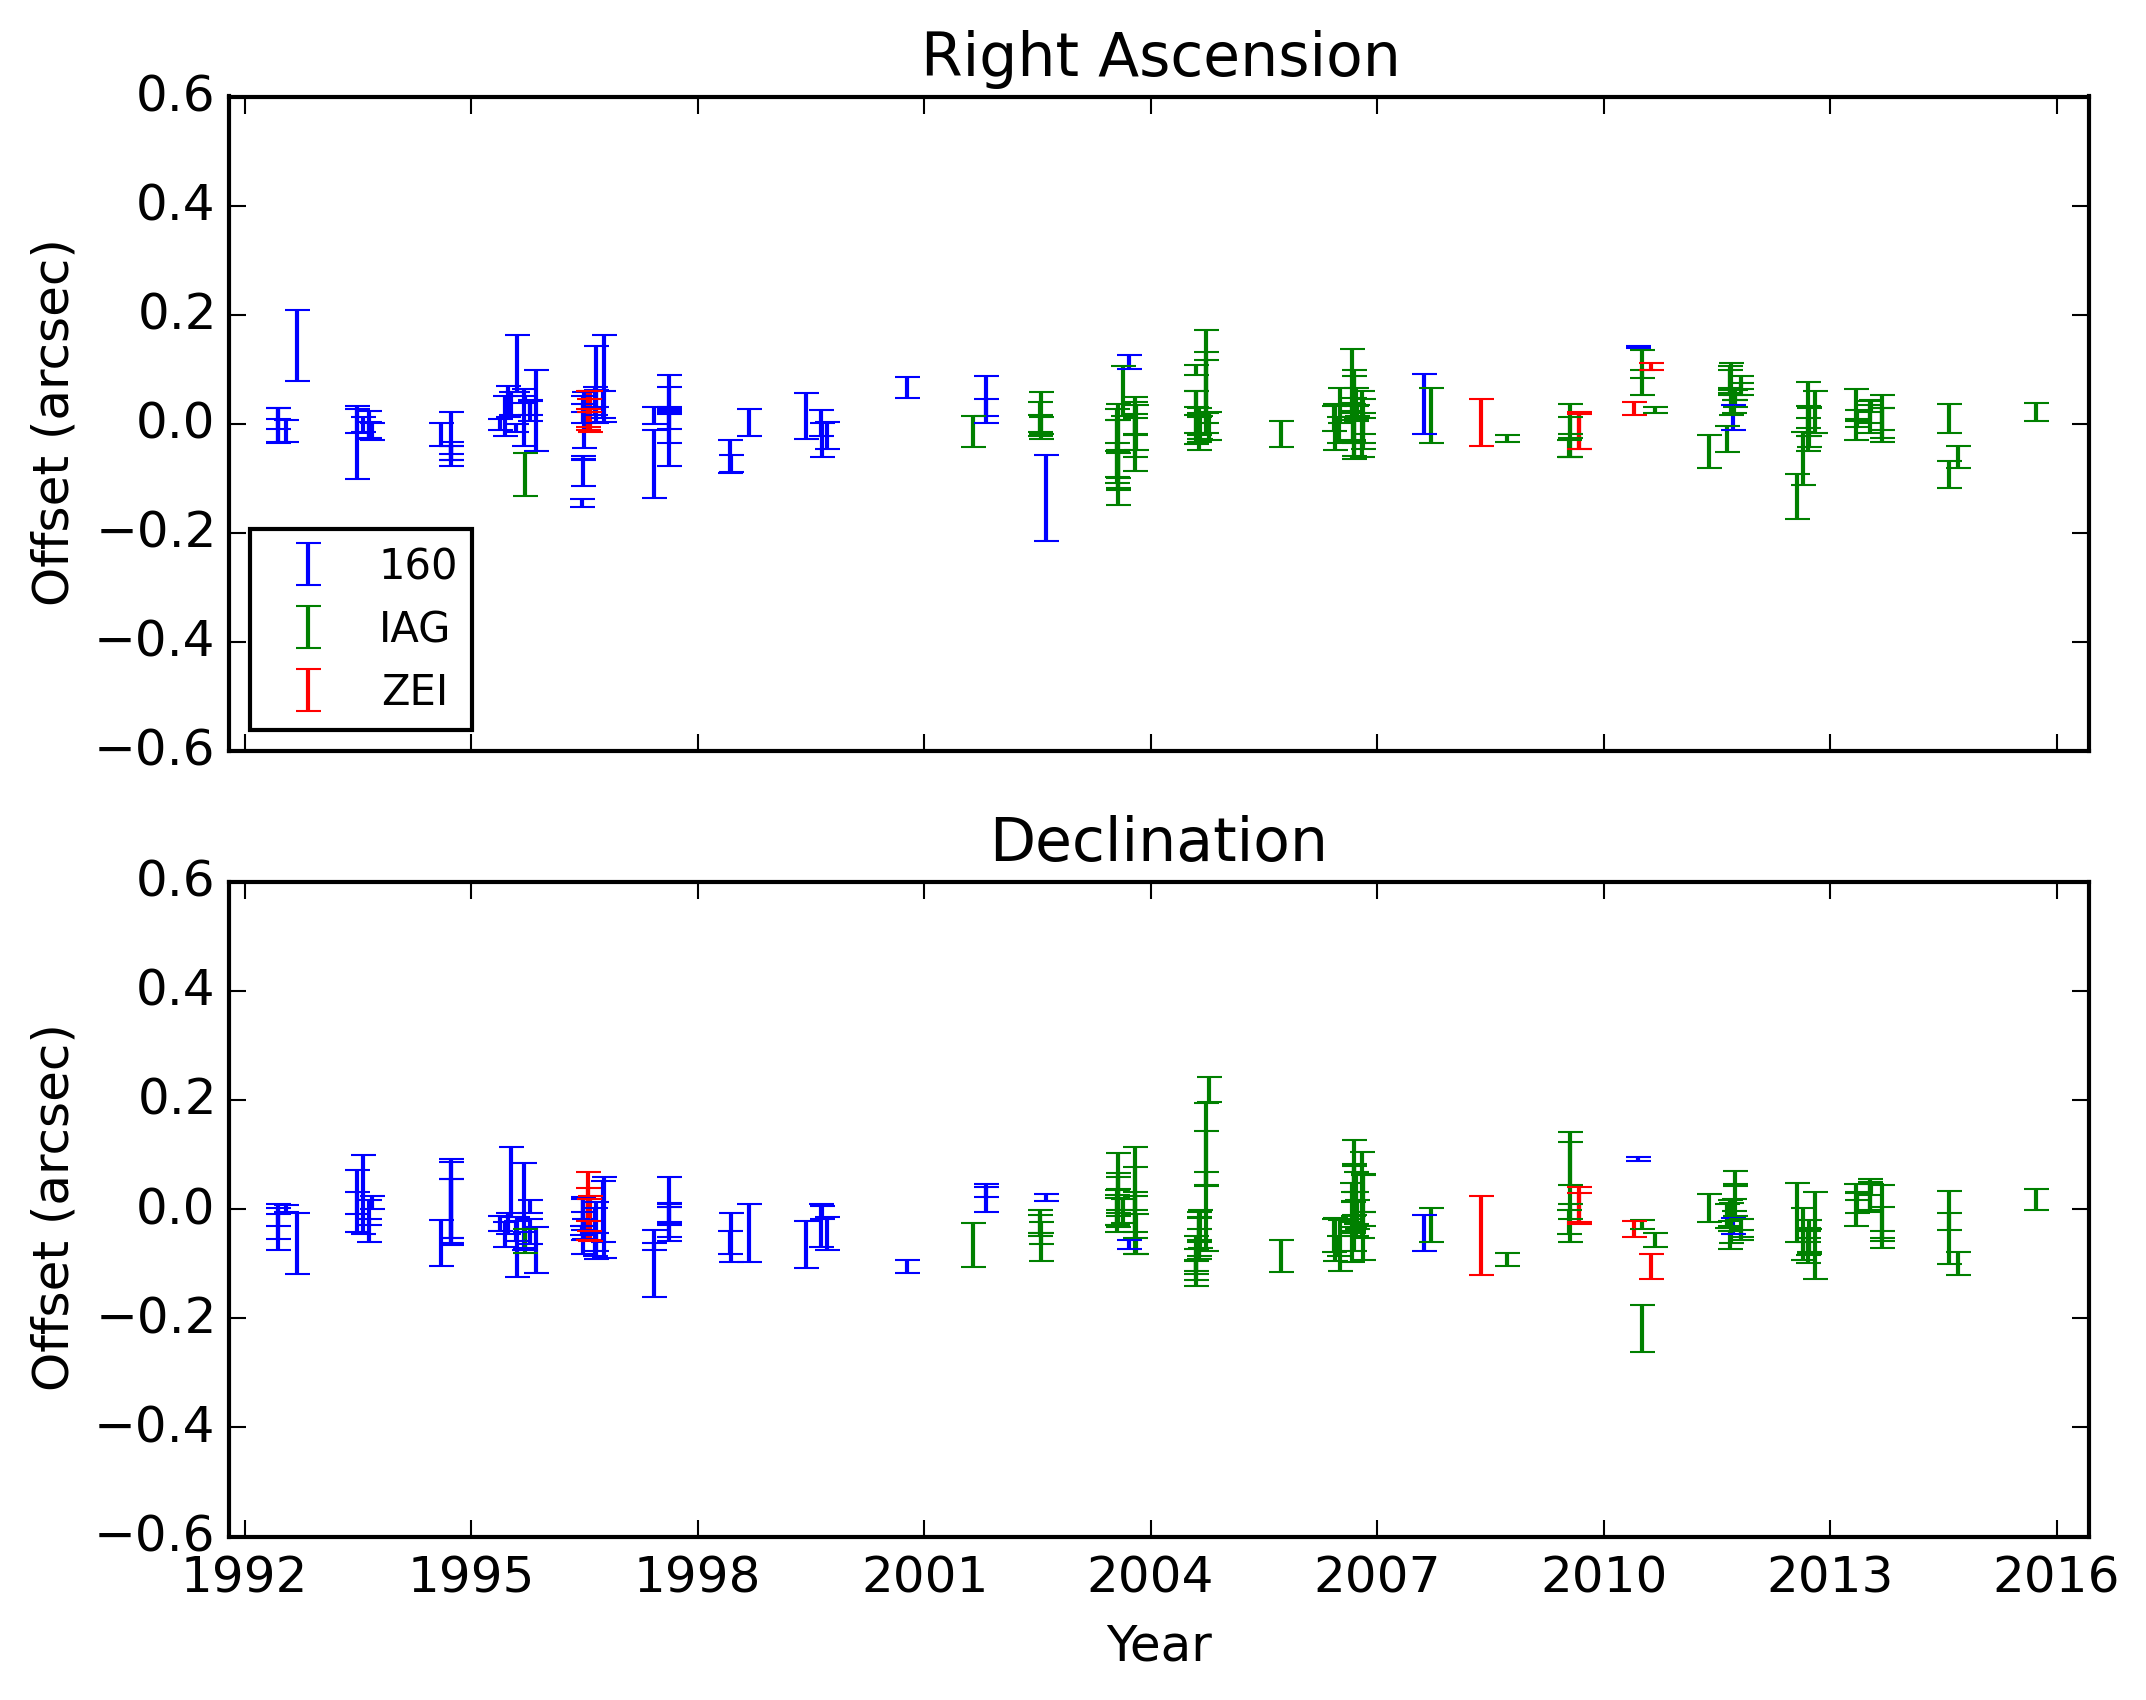
\includegraphics[width=16.0cm]{Triton_media.png} 
%\caption{Triton - Mean offsets by day}
%\label{Fig:trito-media}
%\end{figure}
\begin{figure}
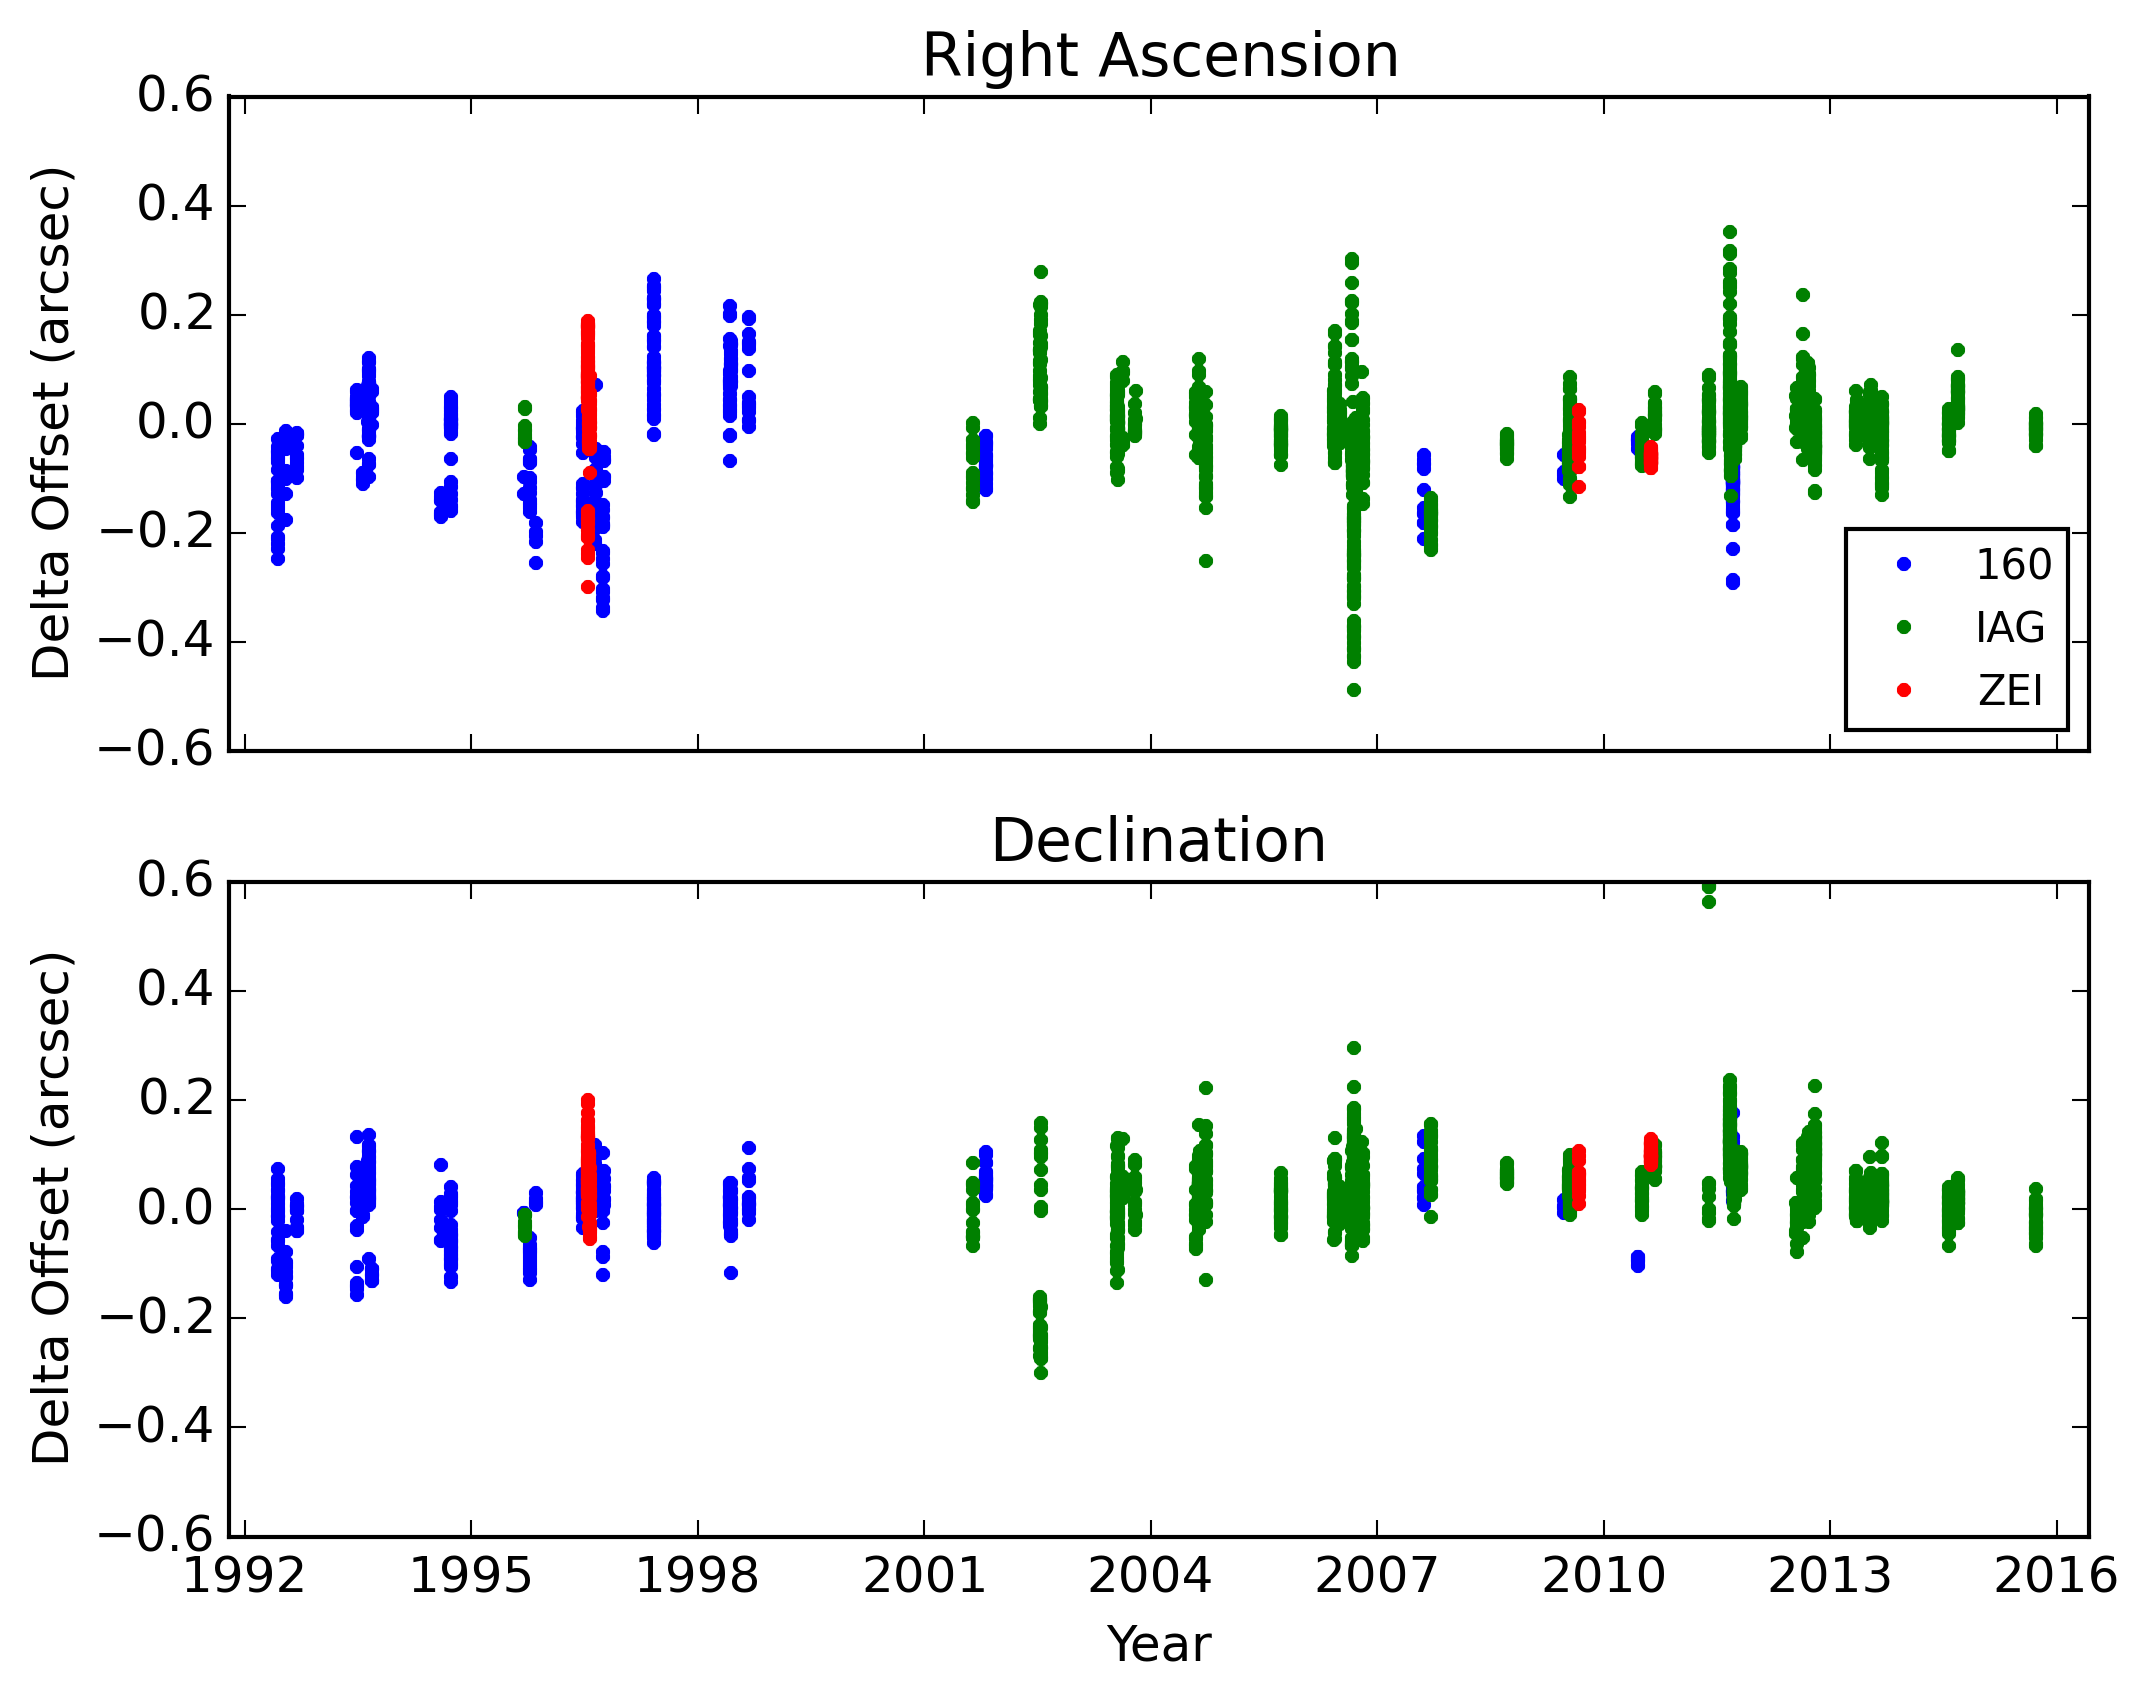
\includegraphics[width=16.0cm]{Triton-Netuno_all.png} 
\caption{Difference between the offsets of Triton and Neptune - All data}
\label{Fig:triton-netuno-all}
\end{figure}
\begin{figure}
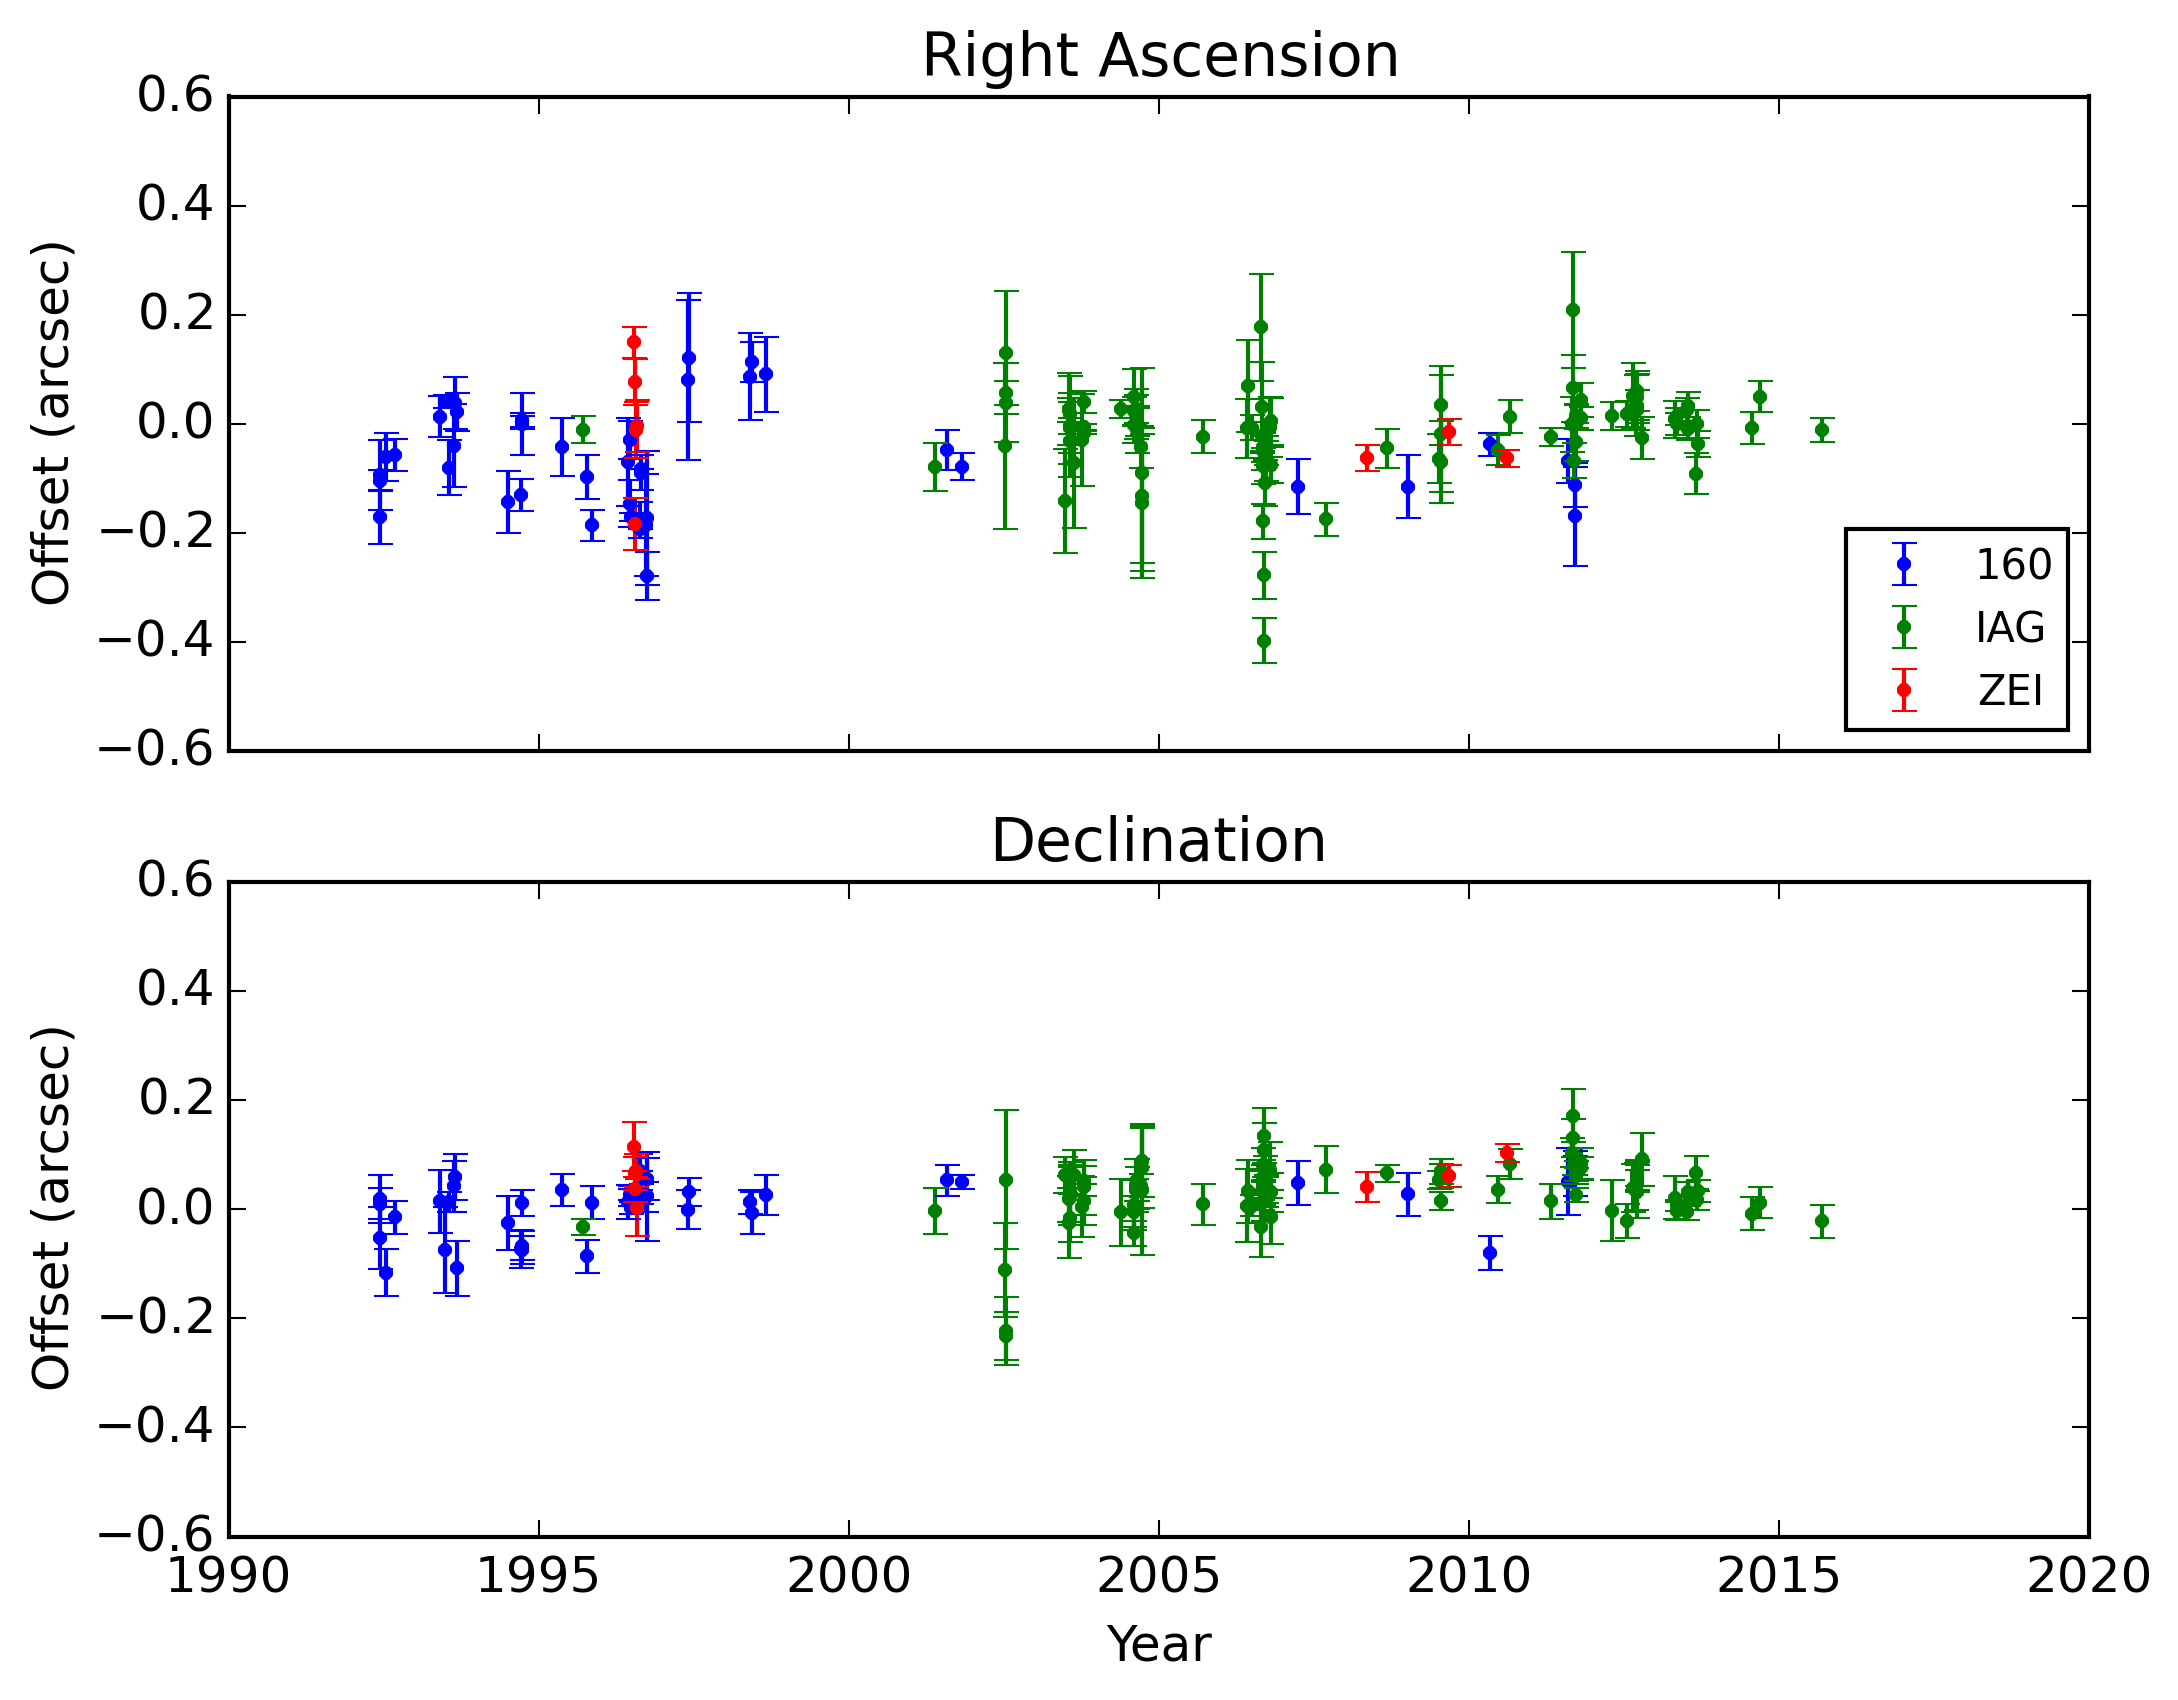
\includegraphics[width=16.0cm]{Triton-Netuno_media.png} 
\caption{Difference between the offsets of Triton and Neptune - Mean offset by day}
\label{Fig:triton-netuno-mean}
\end{figure}


\bibliography{references}
\bibliographystyle{apalike}


\end{document}
